\subsection{Введение в машинное обучение}
	
	\subsubsection{Аннотация}

		Курс <<Введение в машинное обучение>> получил смешанные отзывы.

		Совет студентов и аспирантов ФРКТ просит донести до преподавателей развернутые отзывы респондентов об их работе.
		
		Респонденты отметили, что курс для ФРКТ является достаточно сложным из-за недостатка математических знаний.

		Руководствуясь результатами опроса, Совет студентов и аспирантов ФРКТ выдвигает следующие идеи по улучшению данного курса:
		\begin{enumerate}
			\item необходимо установить чёткие сроки проверки домашних работ и критерии их оценивания;
			\item необходимо заранее публиковать расписание курса, включая даты экзаменов и зачётов, и соблюдать его.
		\end{enumerate}
				

	\subsubsection{Общий отзыв студентов о курсе}

		\begin{figure}[H]
			\centering
			\begin{subfigure}[b]{0.45\textwidth}
				\centering
				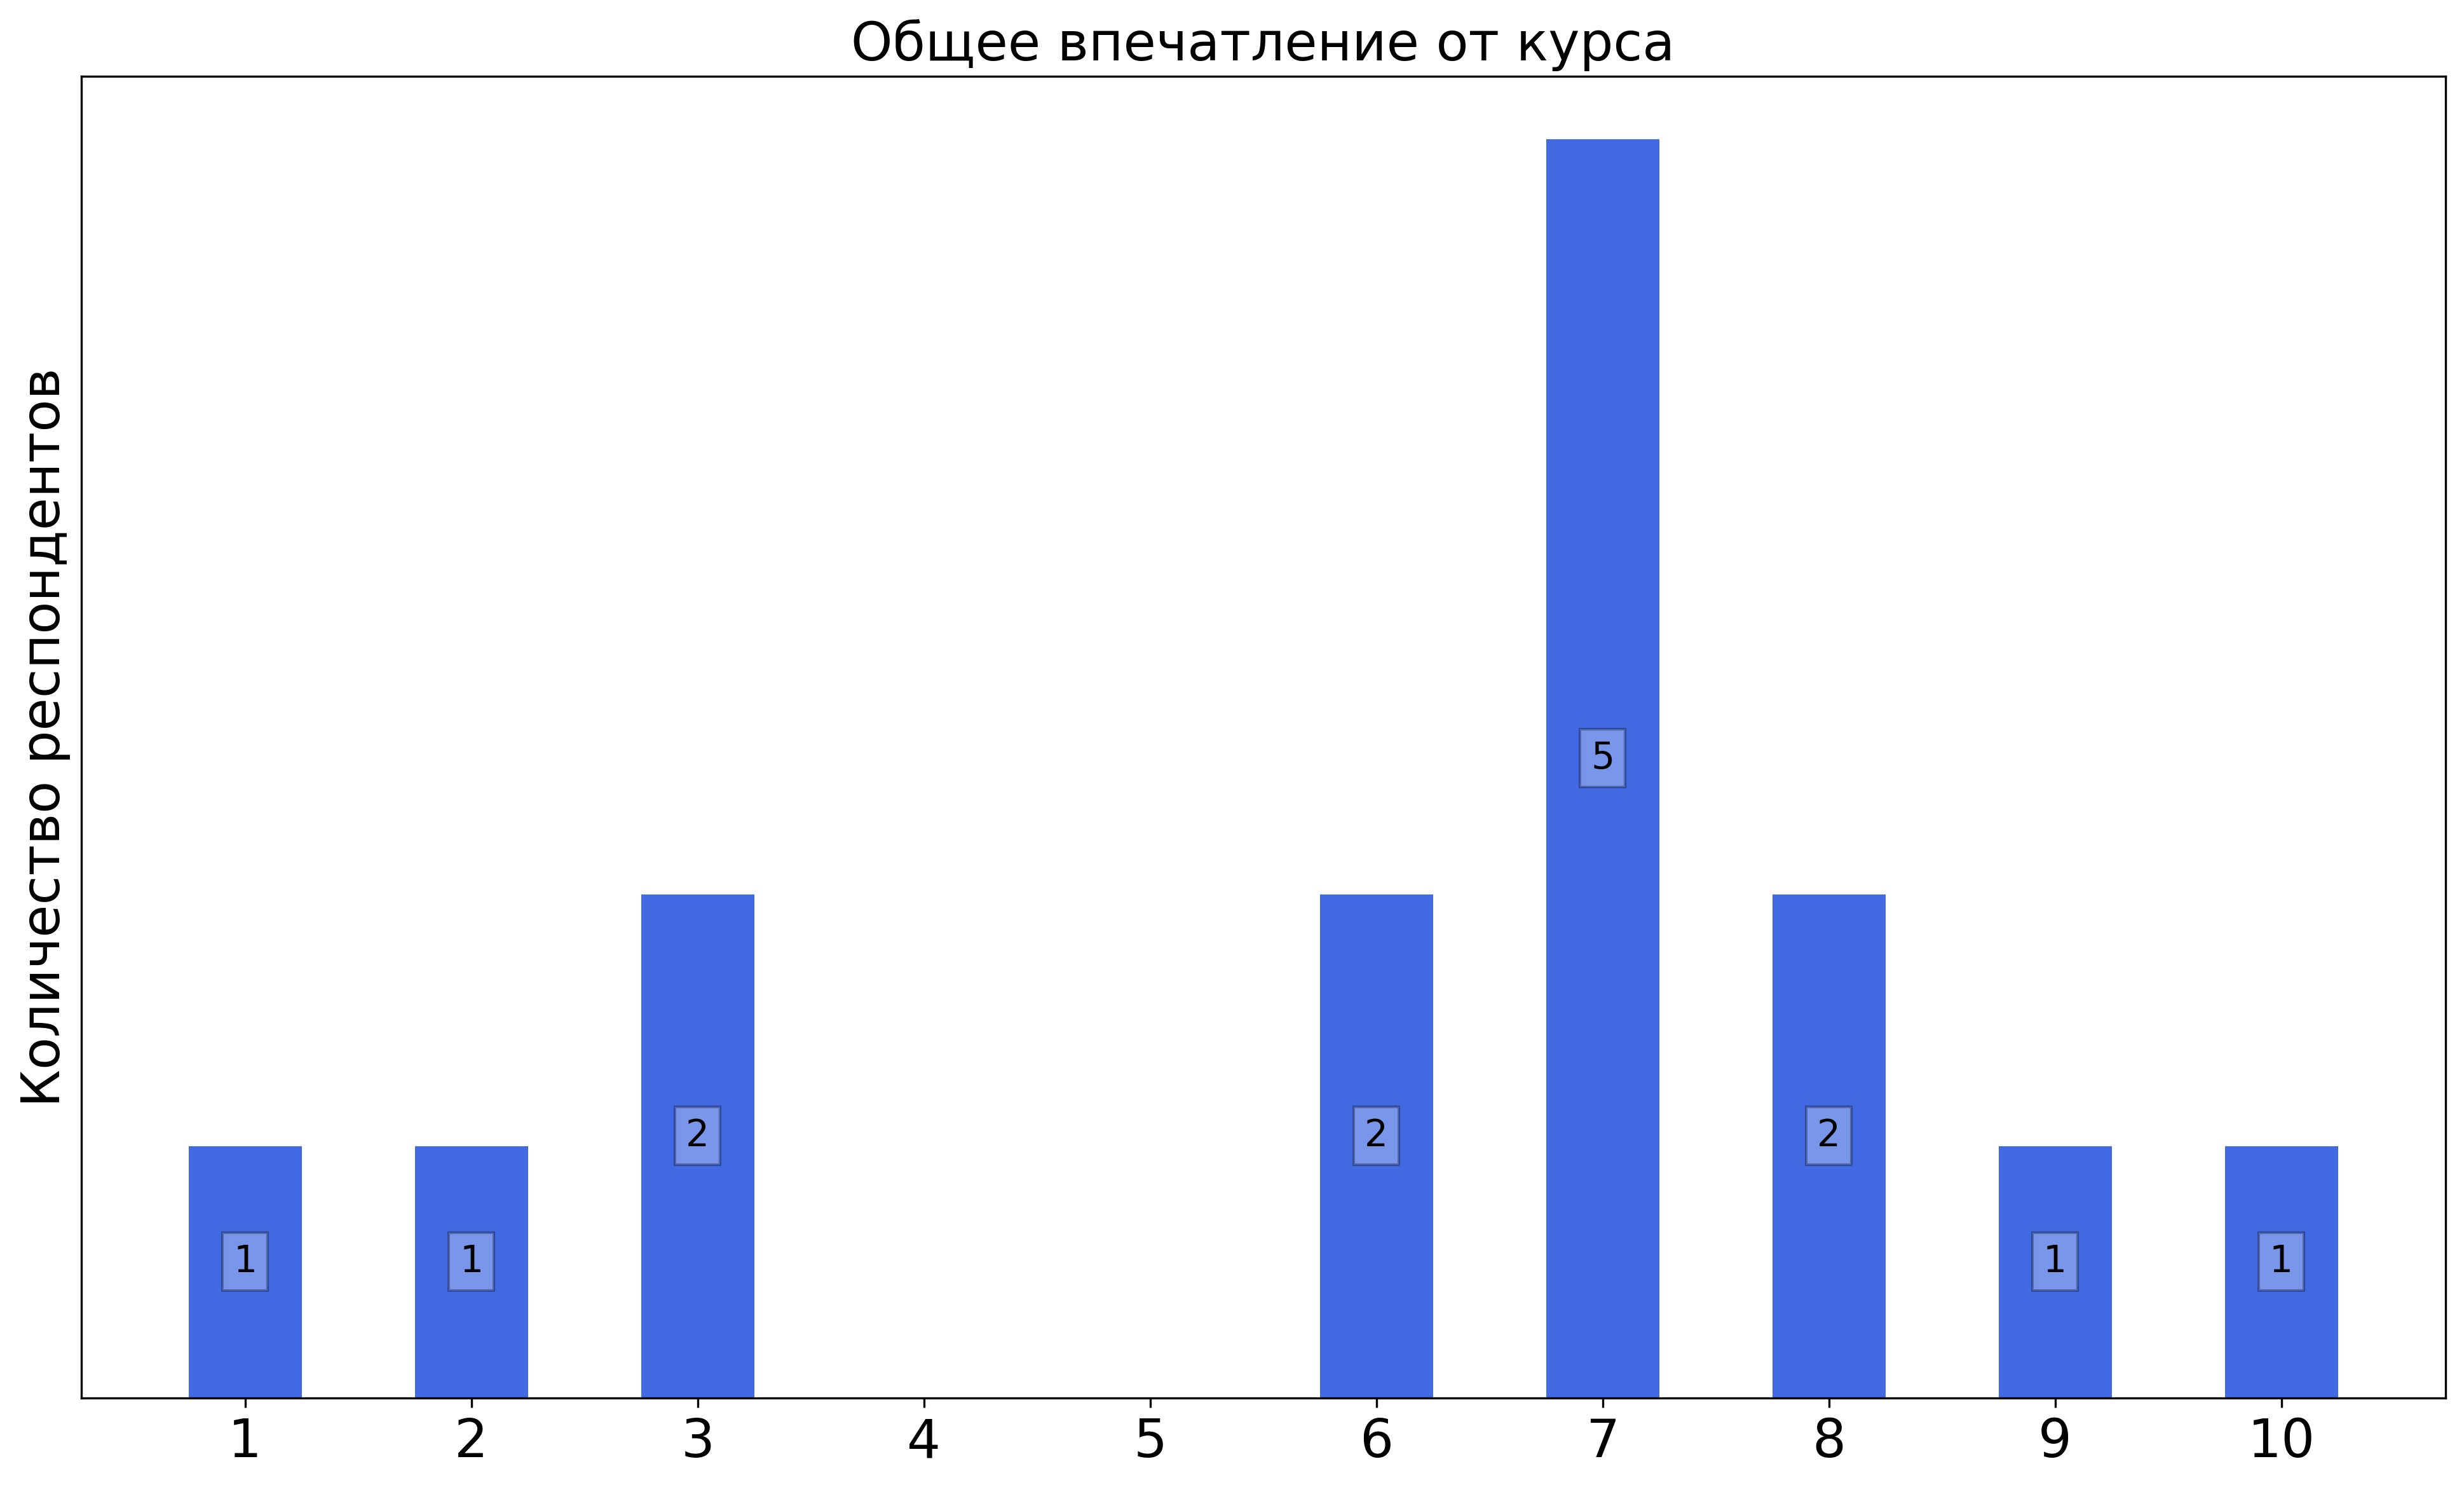
\includegraphics[width=\textwidth]{images/4 course/Введение в машинное обучение/general-0.png}
			\end{subfigure}
			\begin{subfigure}[b]{0.45\textwidth}
				\centering
				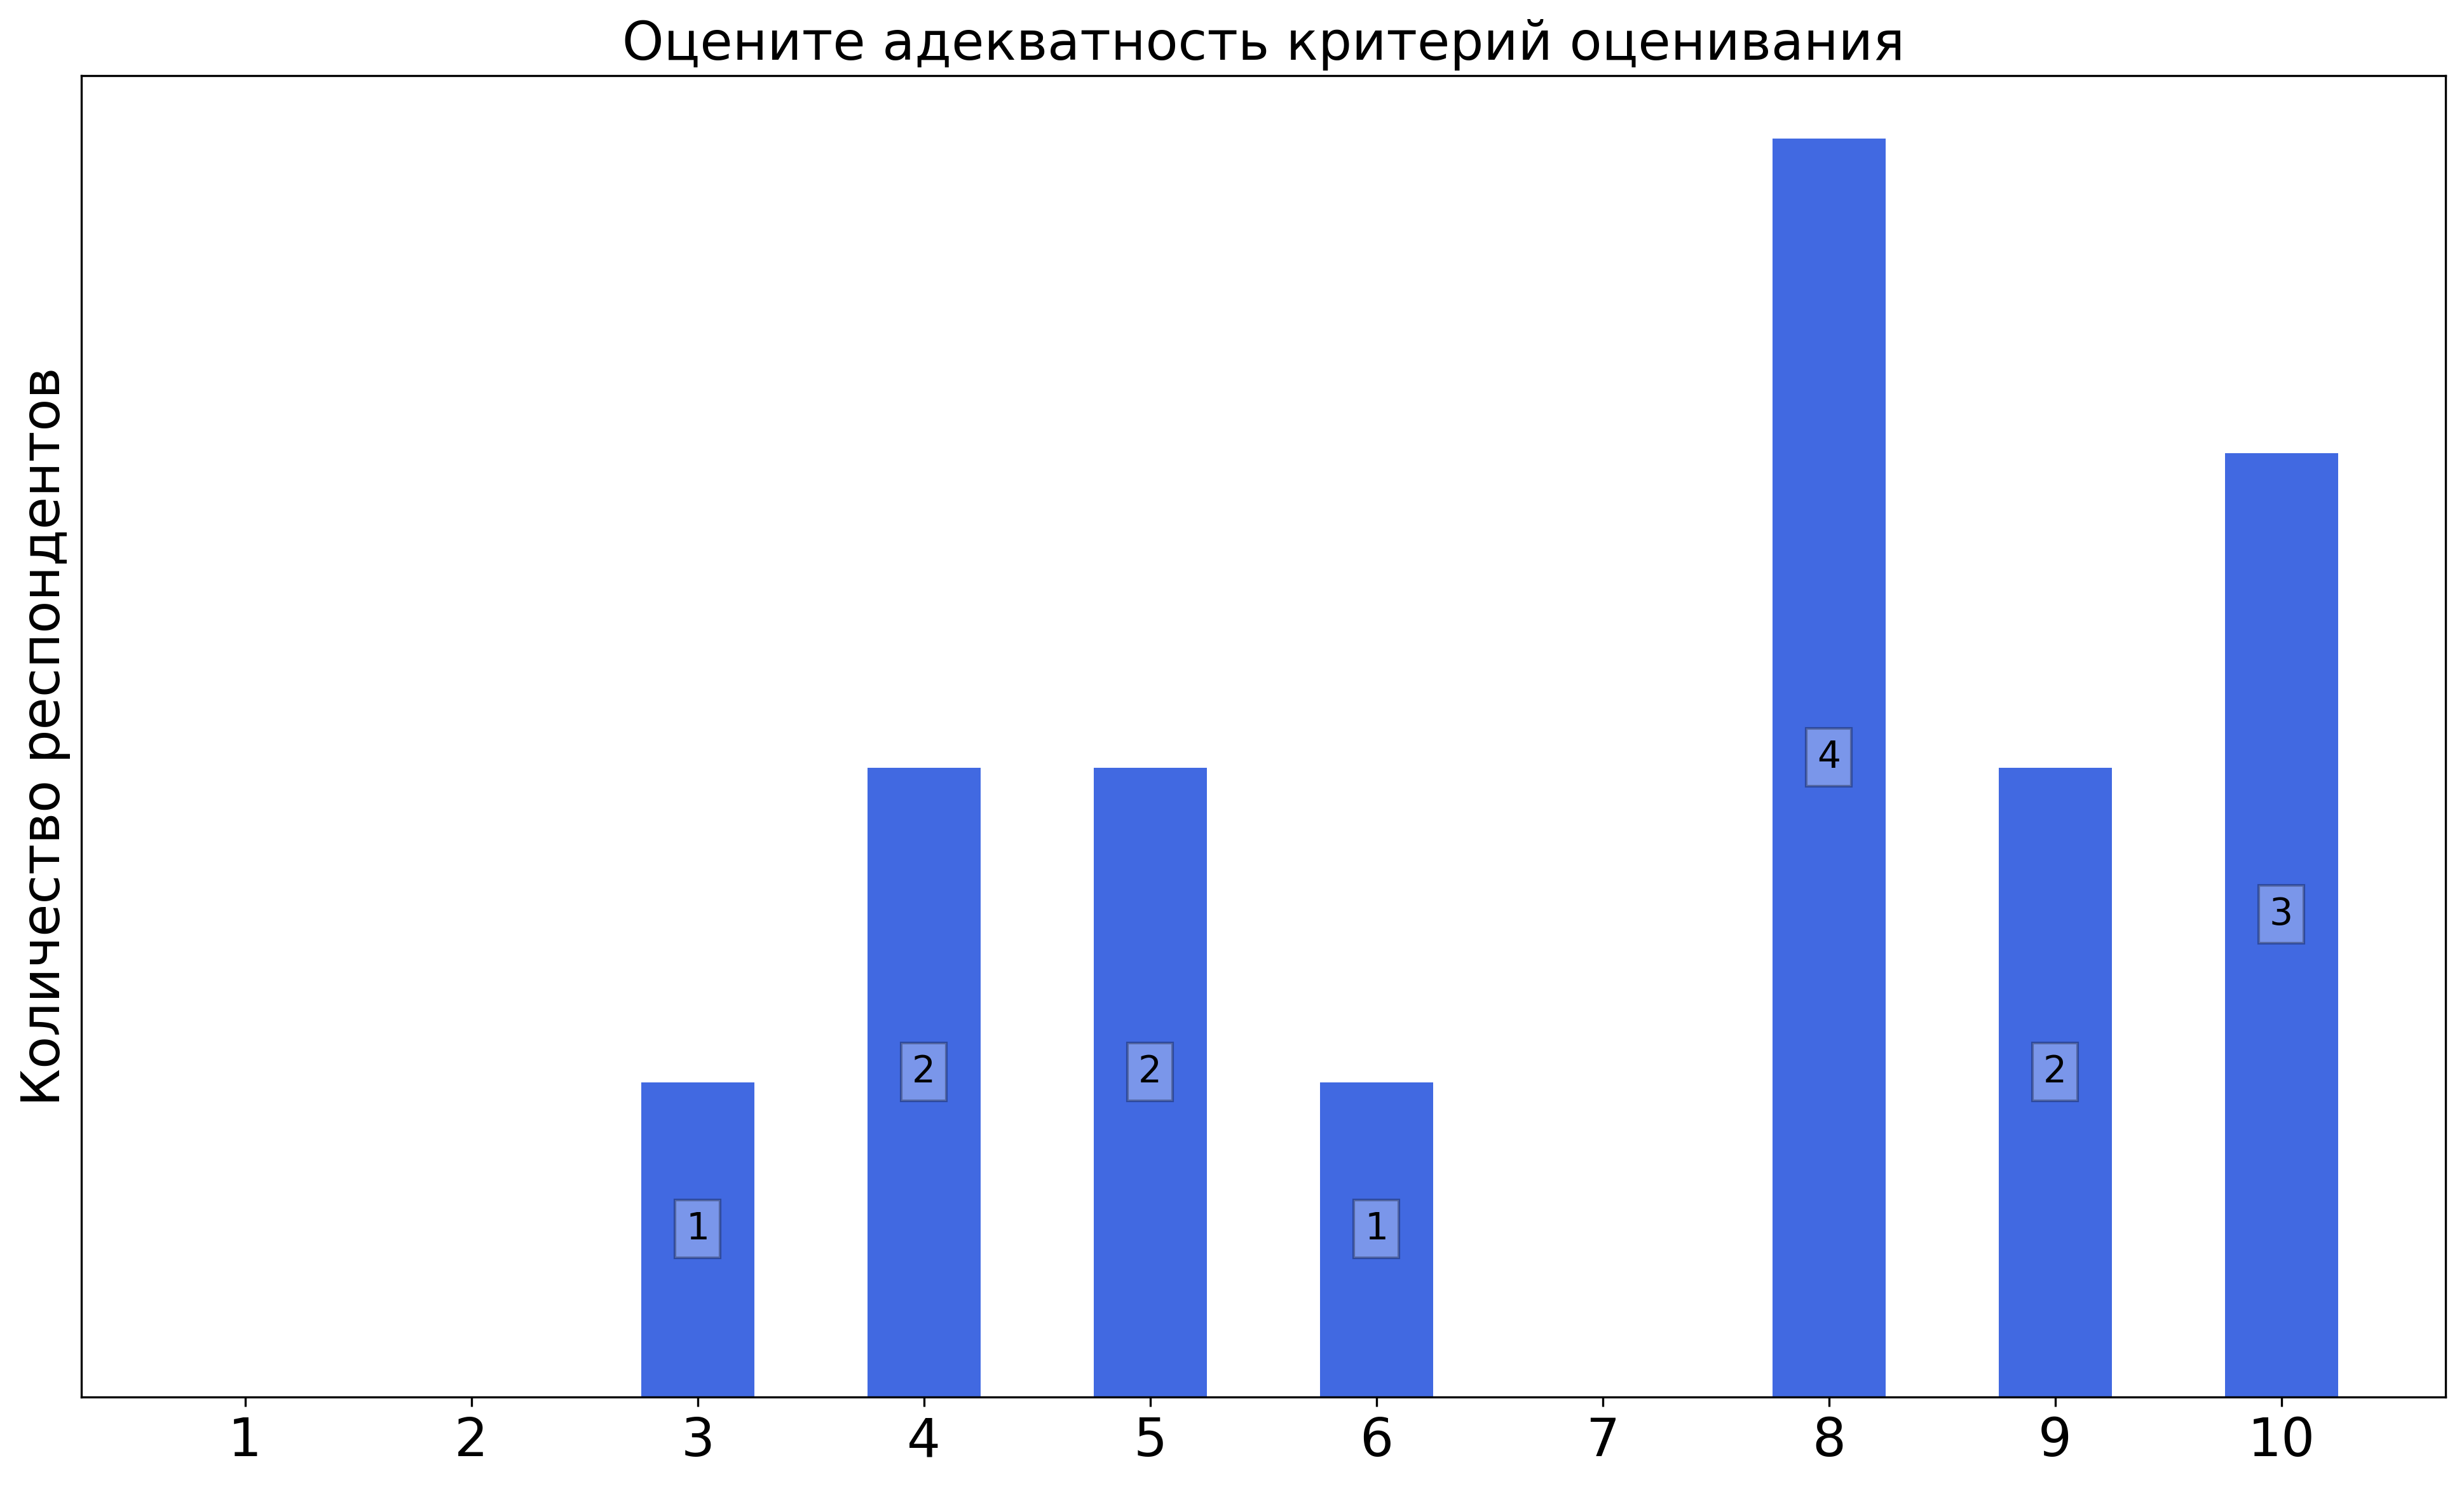
\includegraphics[width=\textwidth]{images/4 course/Введение в машинное обучение/general-1.png}
			\end{subfigure}	
		\end{figure}

	\subsubsection{Материалы, использумые респондентами при изучении курса}

		\begin{figure}[H]
			\centering
			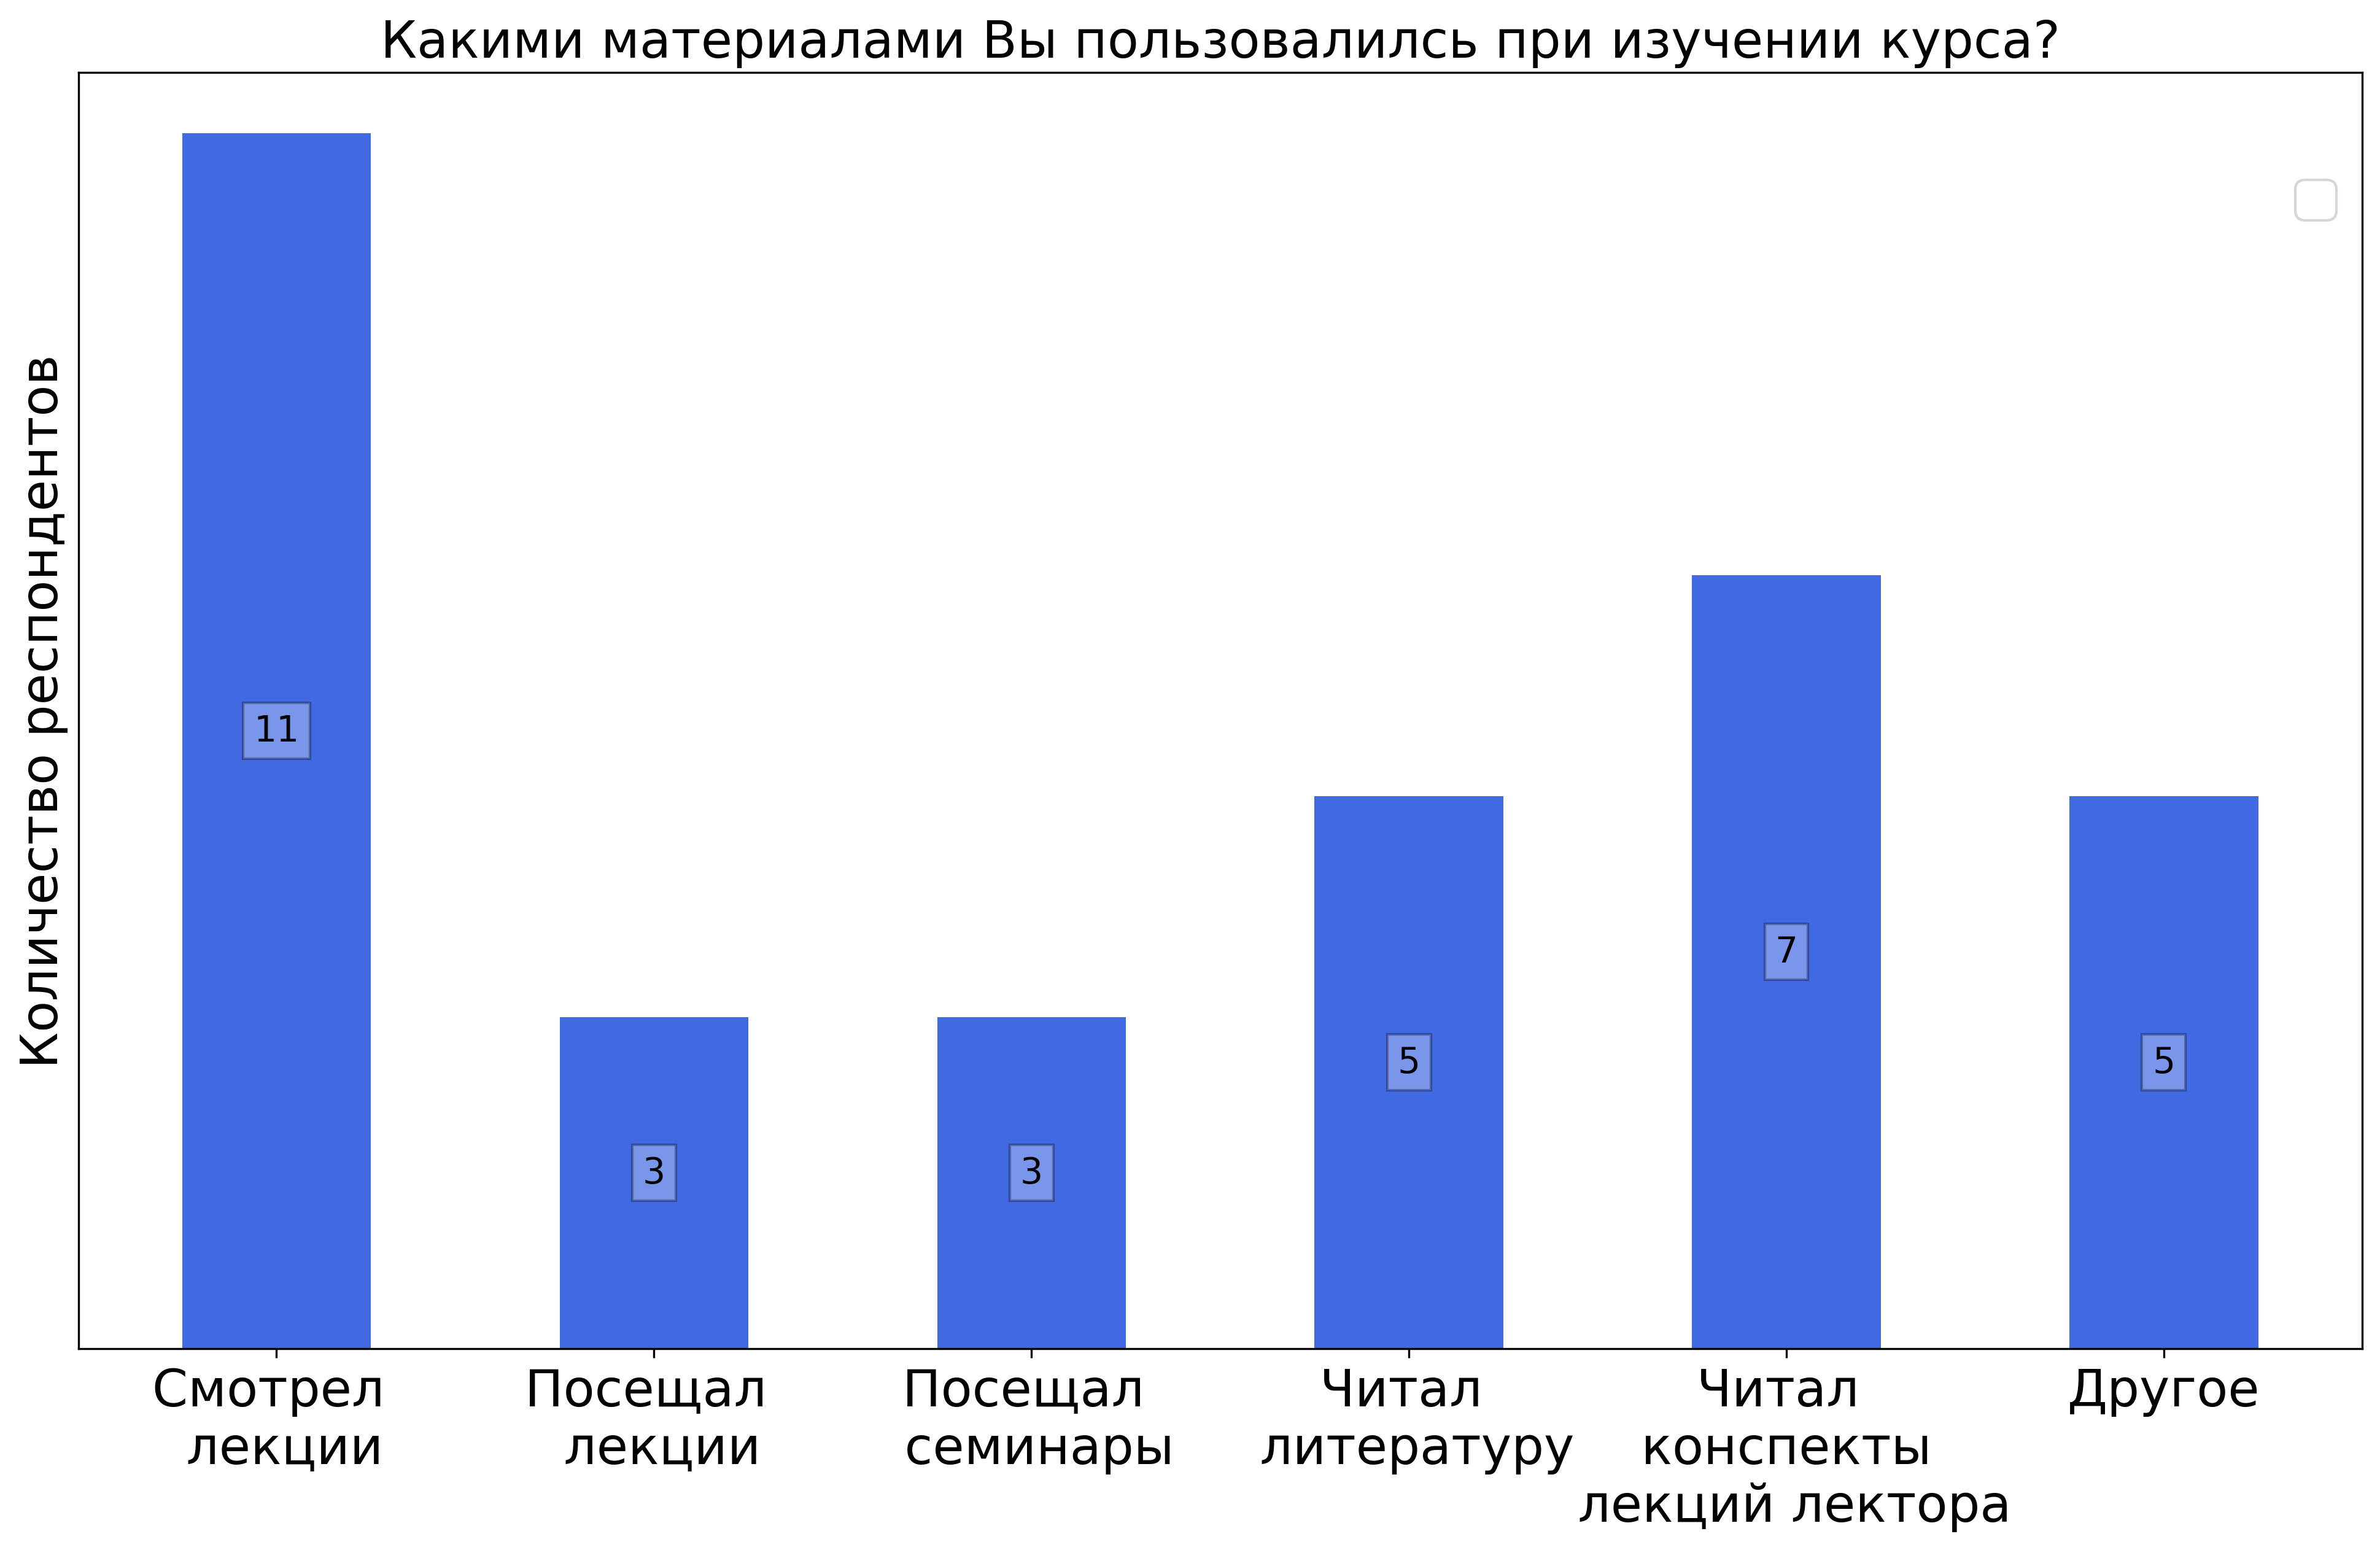
\includegraphics[width = 0.45\textwidth]{images/4 course/Введение в машинное обучение/materials.png}
		\end{figure}

		\textit{В качестве других источников информации студенты указали:} 
		\begin{itemize}
			\item курс Deep Learning School;
			\item хендбук от "Яндекс";
			\item слайды презентаций, которые показывали на лекциях;
			\item консультации с коллегами на работе.
		\end{itemize}

	\subsubsection{Отзыв студентов о лекциях. Лектор: Воронцов К.В..}
		\begin{figure}[H]
			\centering
            \begin{subfigure}[b]{0.45\textwidth}
				\centering
				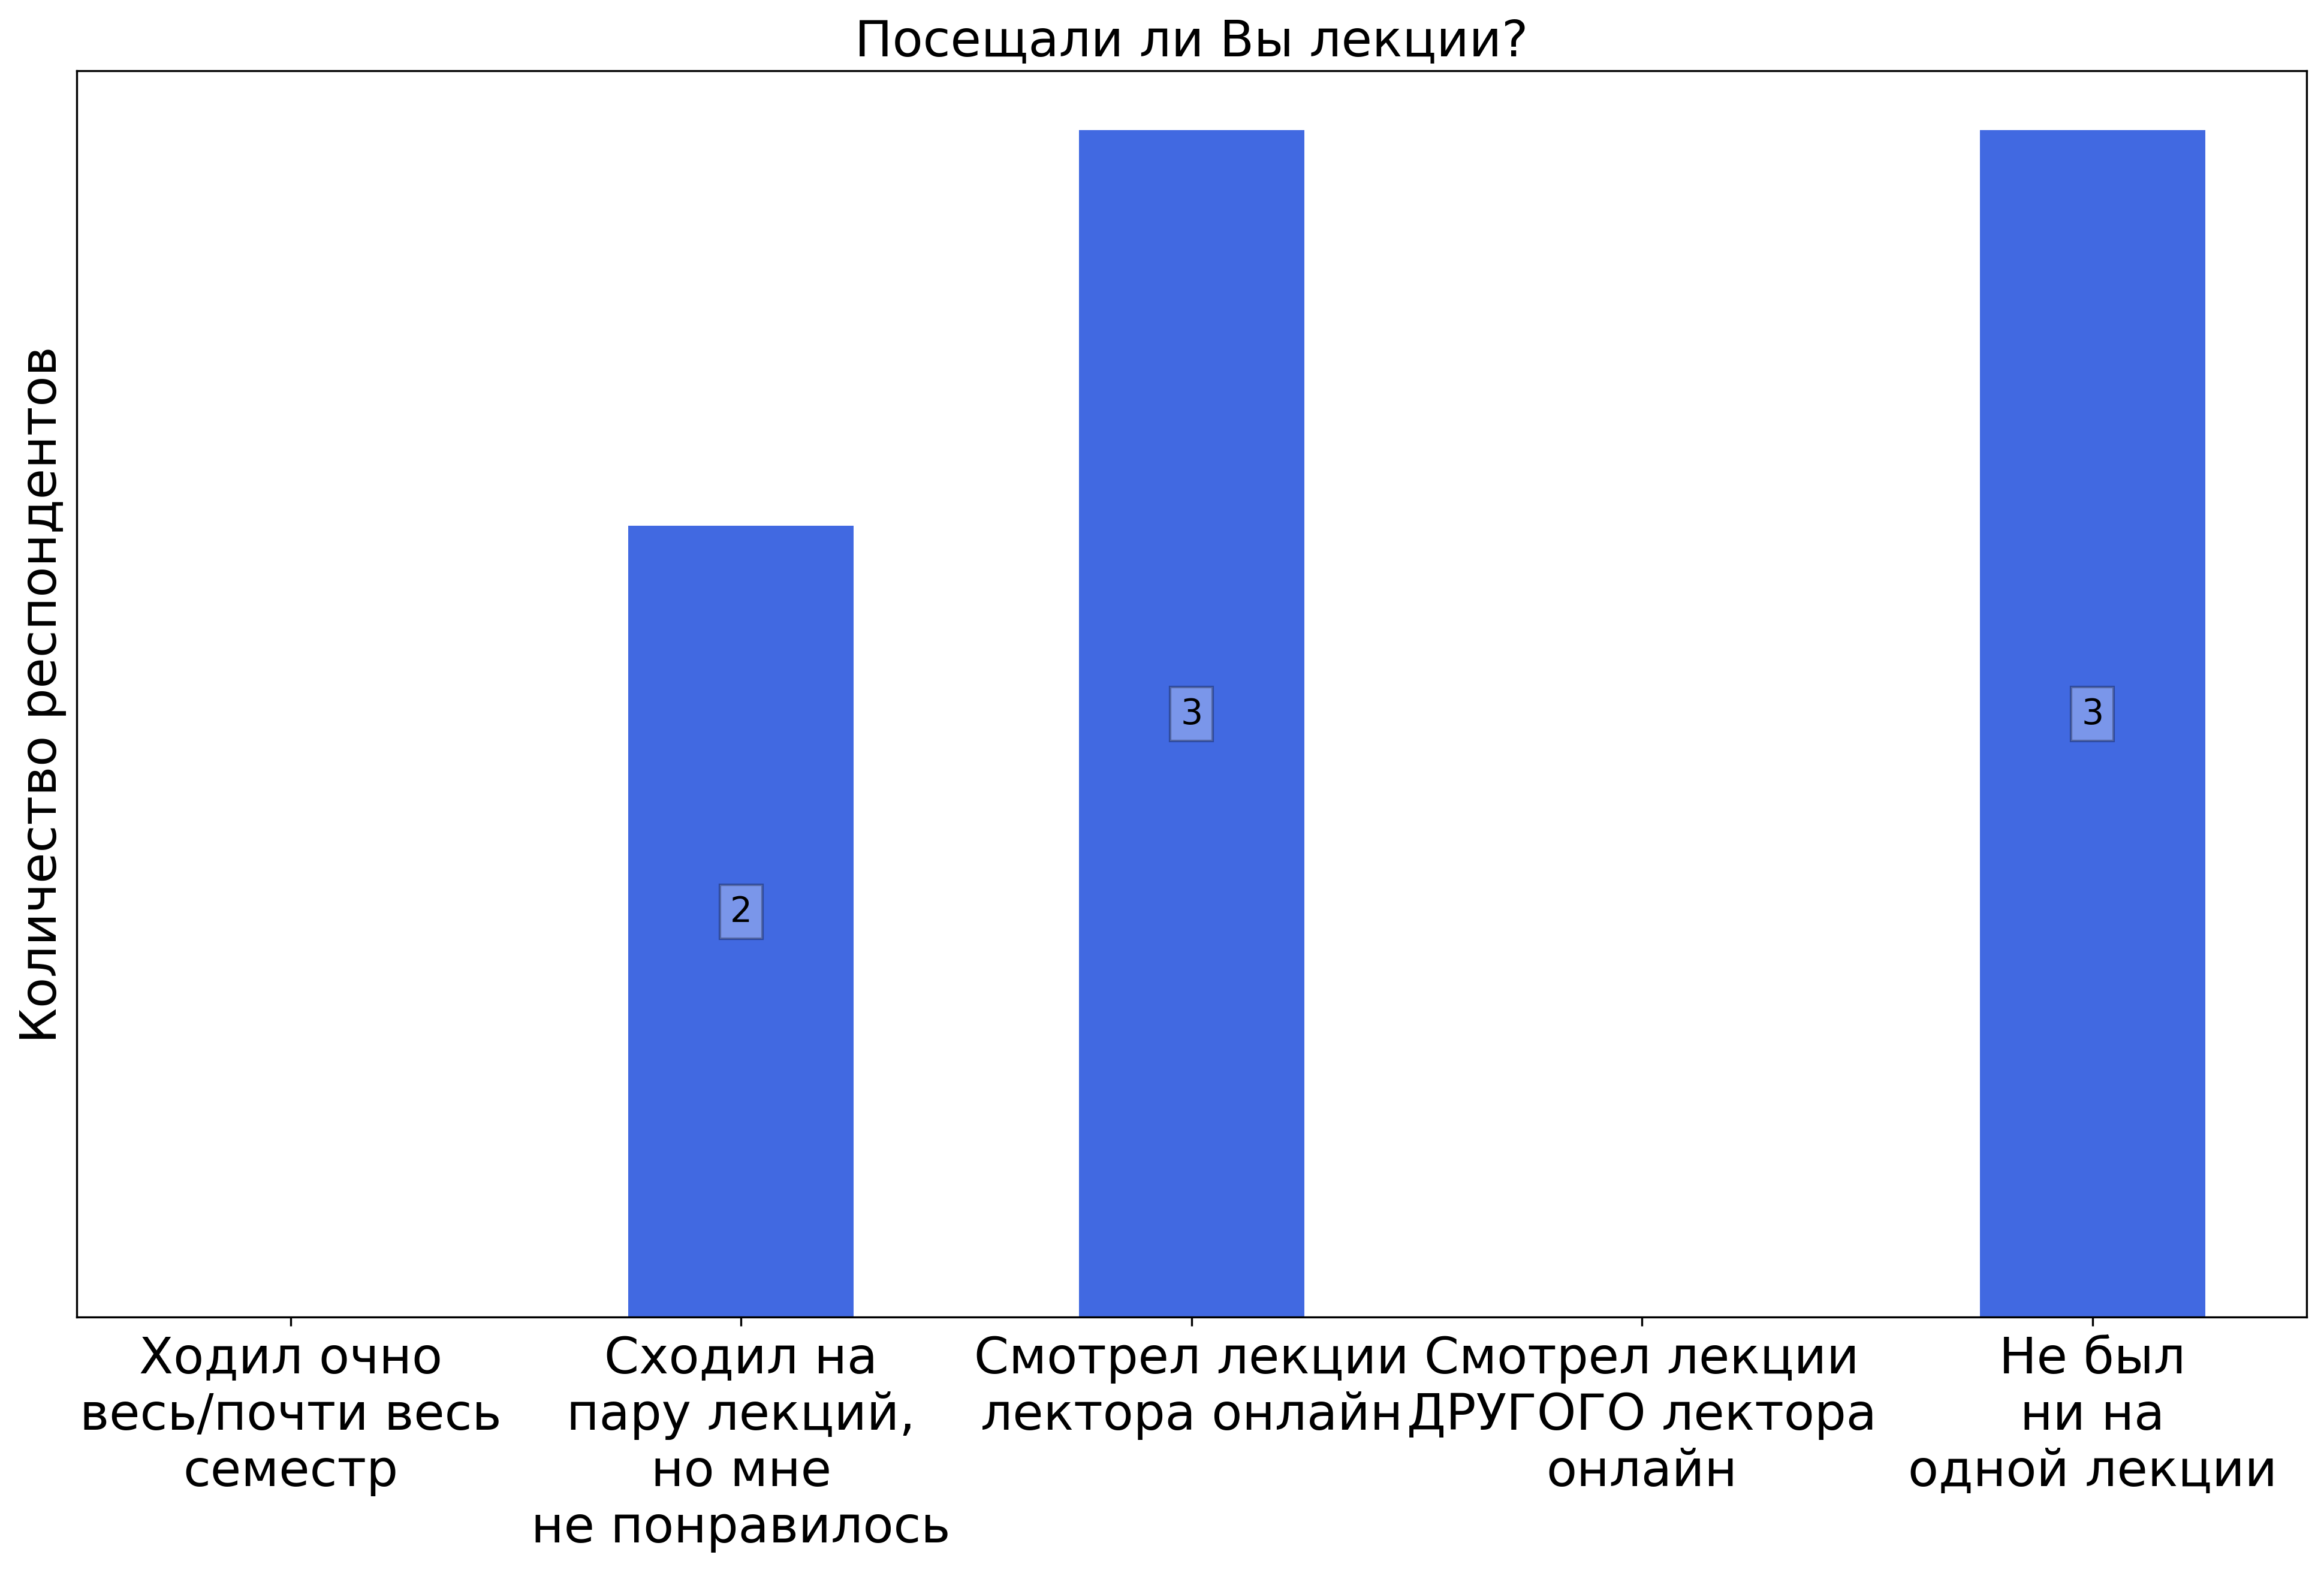
\includegraphics[width=\textwidth]{images/4 course/Введение в машинное обучение/lecturer-questions-Воронцов К.В.-0.png}
			\end{subfigure}
			\begin{subfigure}[b]{0.45\textwidth}
				\centering
				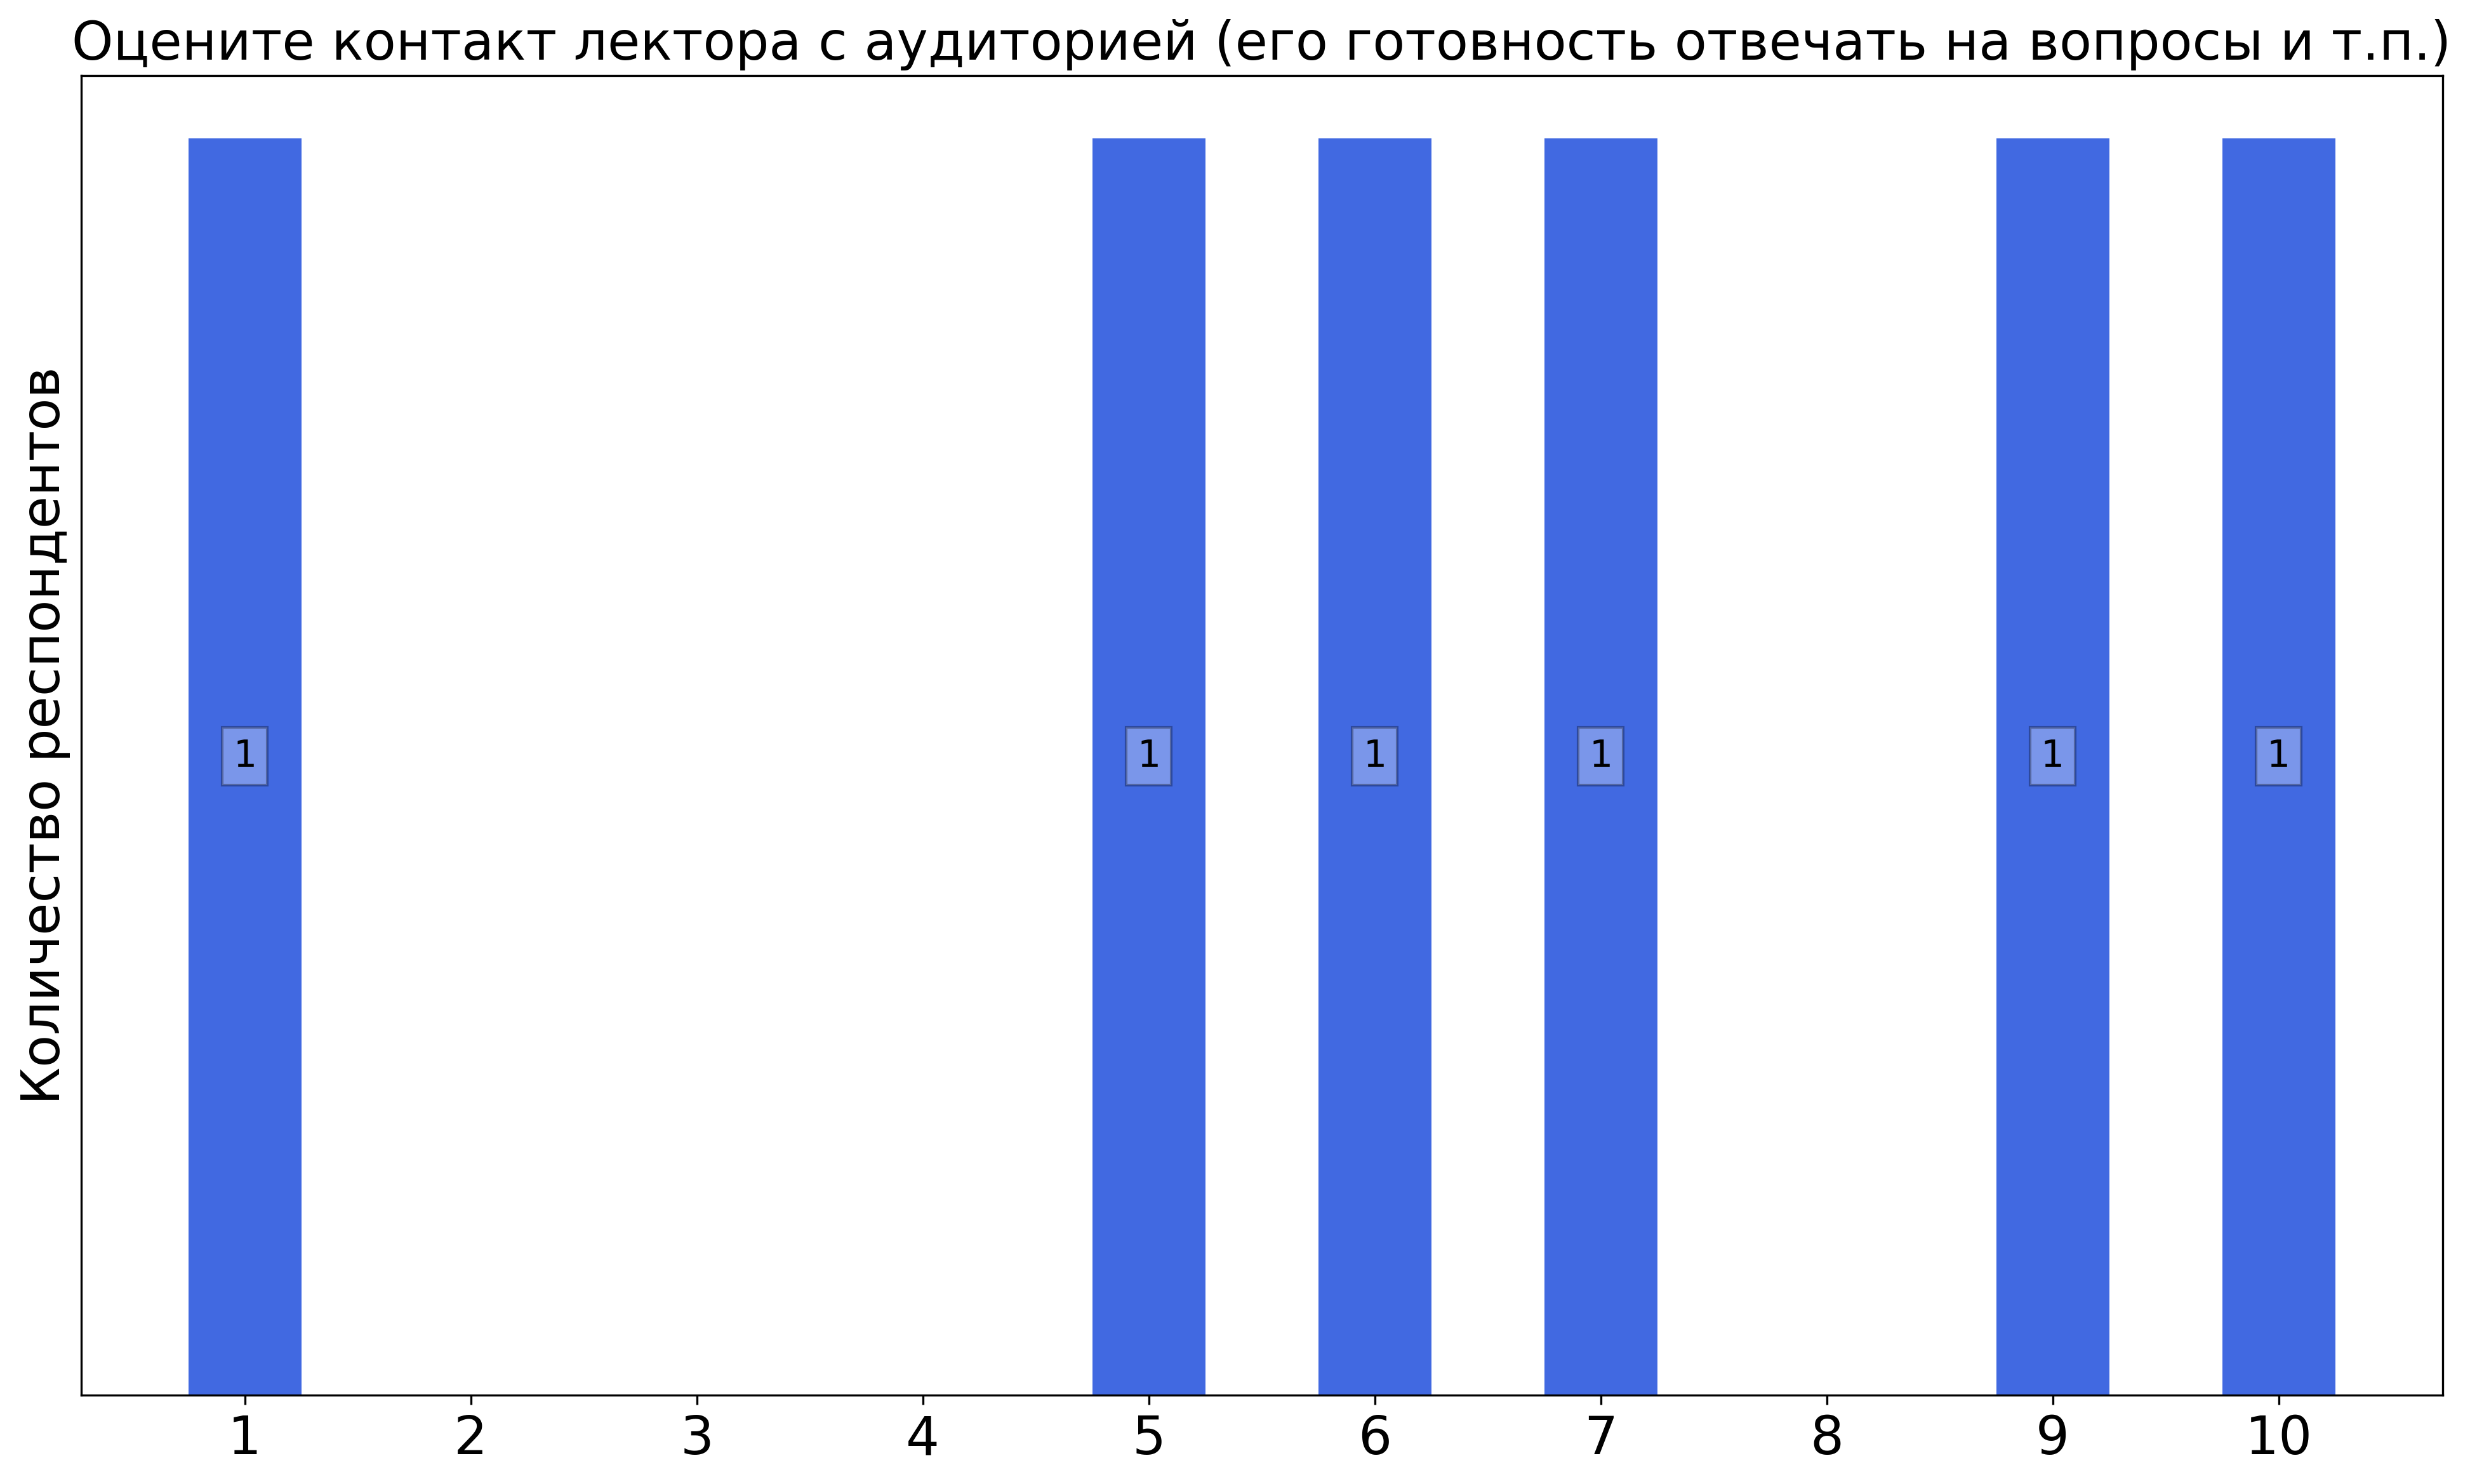
\includegraphics[width=\textwidth]{images/4 course/Введение в машинное обучение/lecturer-marks-Воронцов К.В.-0.png}
			\end{subfigure}
			\begin{subfigure}[b]{0.45\textwidth}
				\centering
				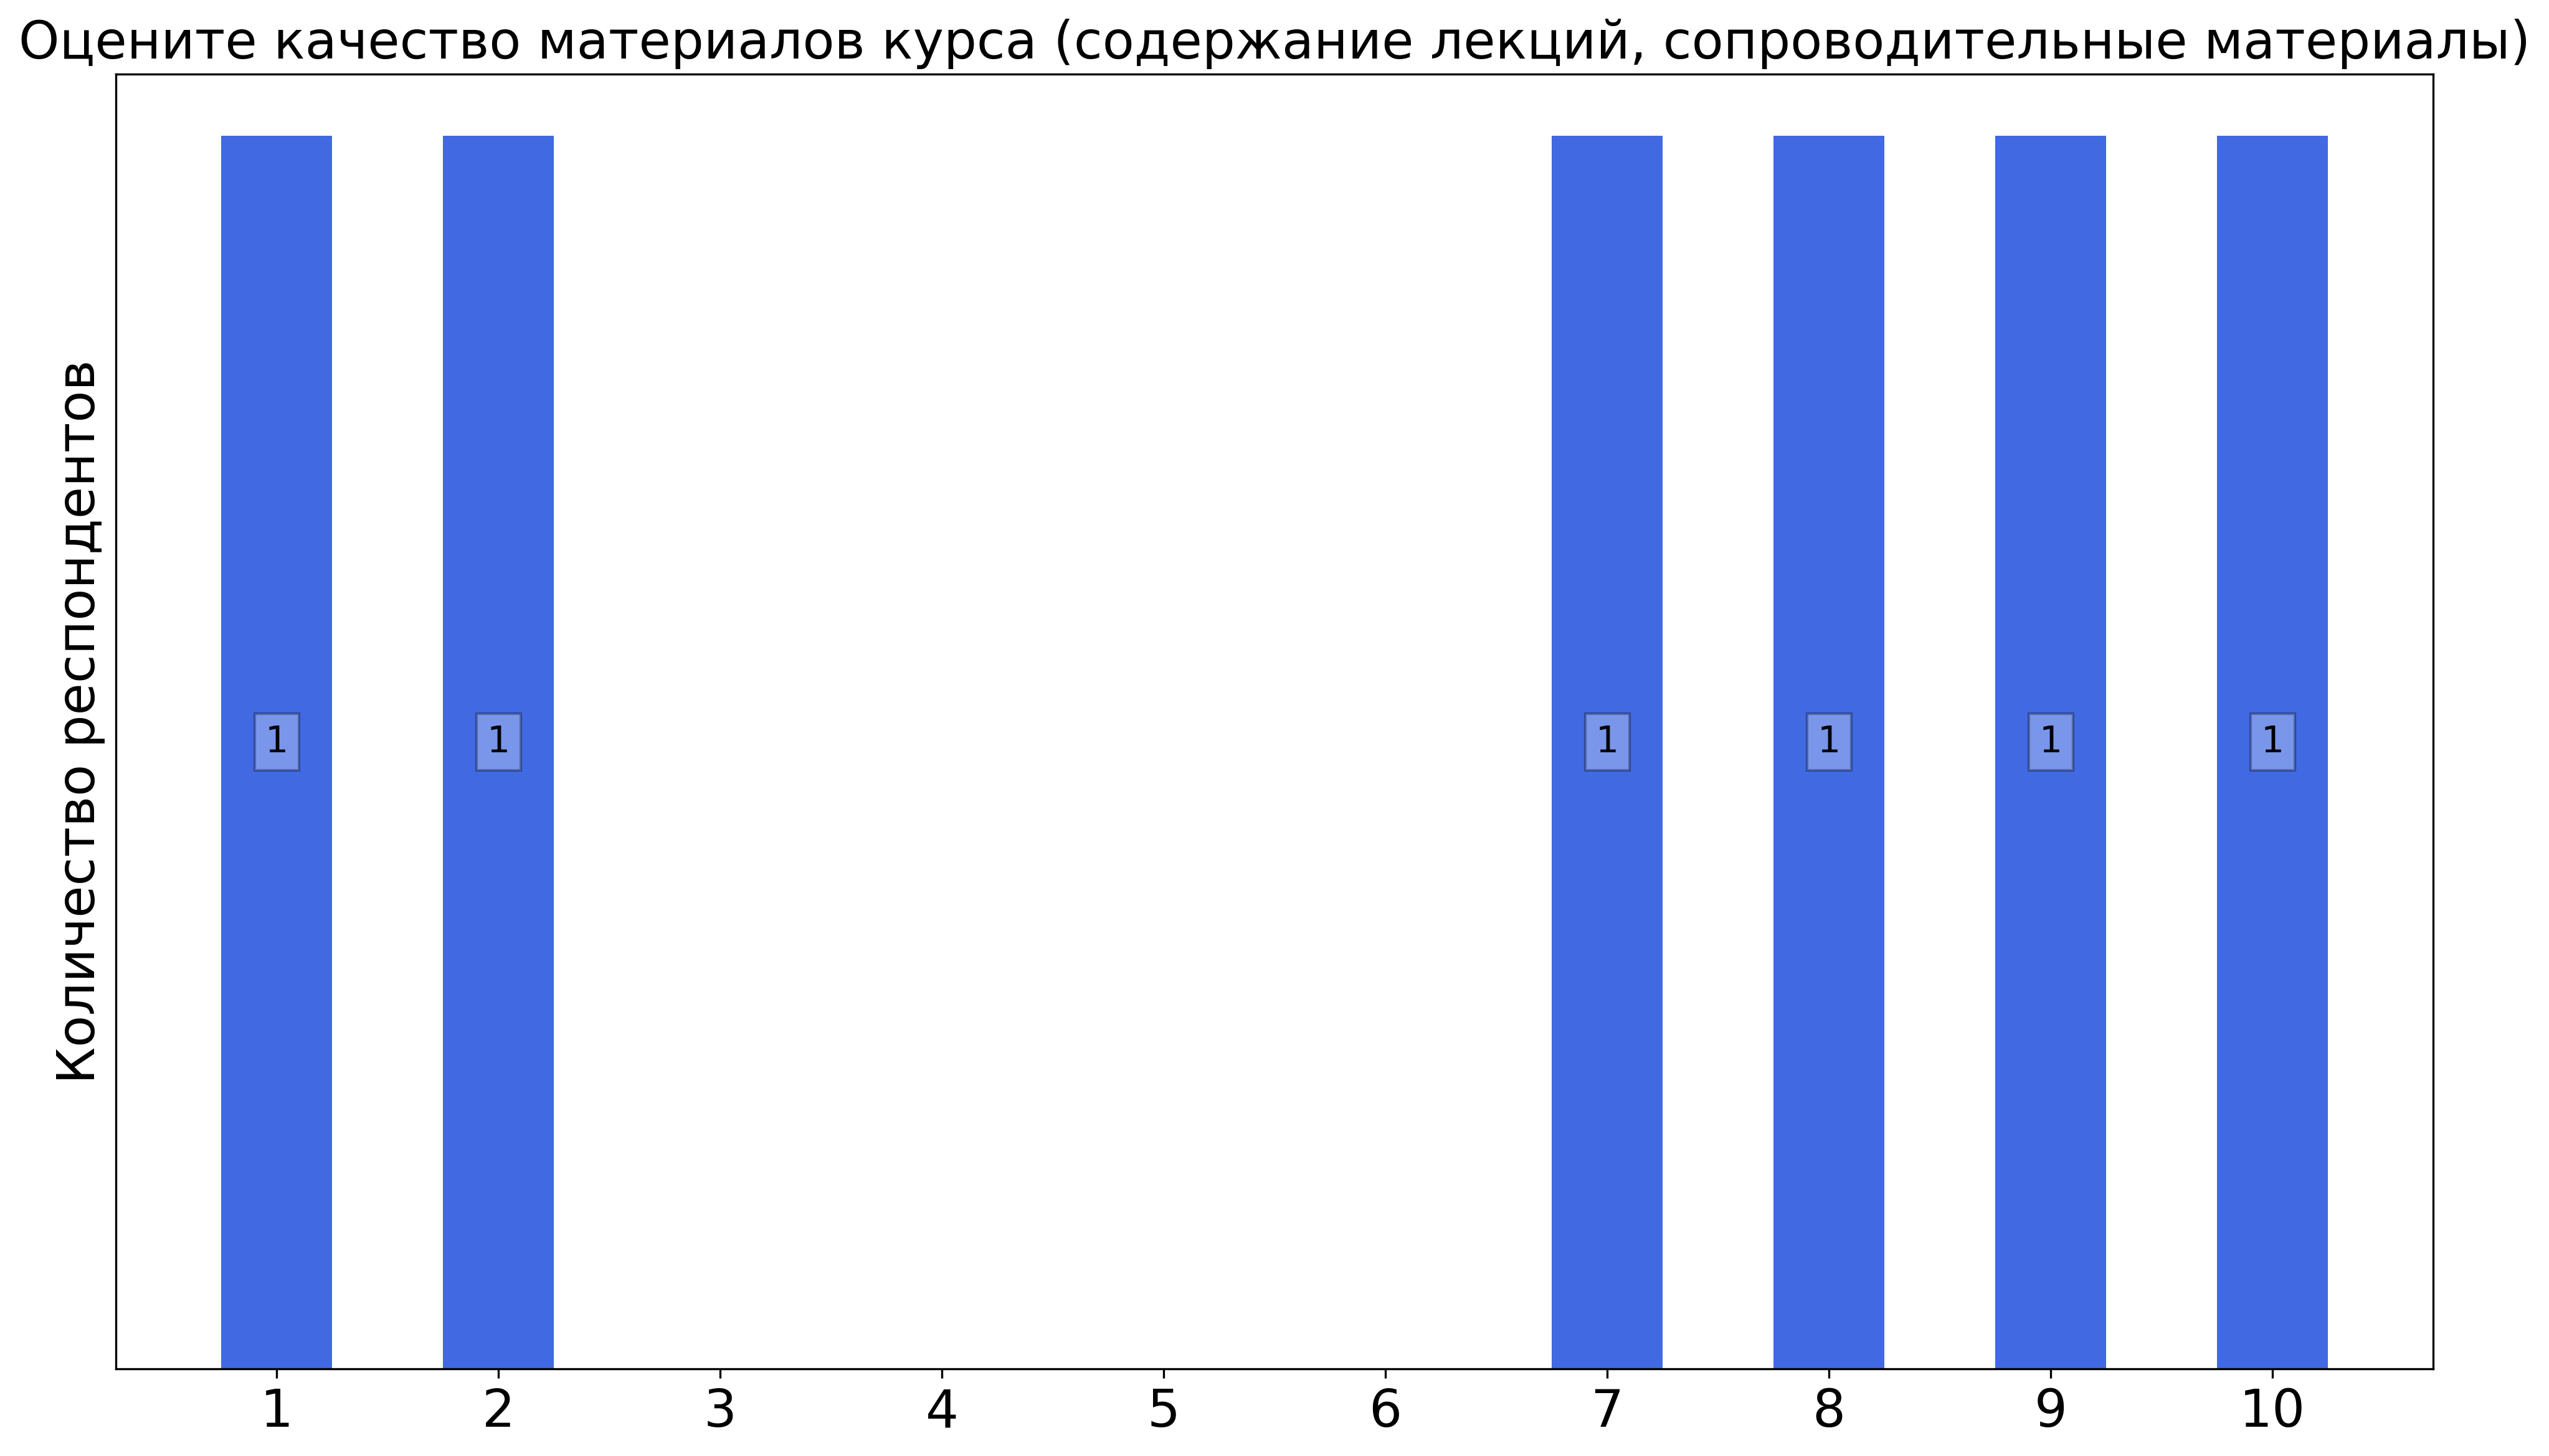
\includegraphics[width=\textwidth]{images/4 course/Введение в машинное обучение/lecturer-marks-Воронцов К.В.-1.png}
			\end{subfigure}
			\begin{subfigure}[b]{0.45\textwidth}
				\centering
				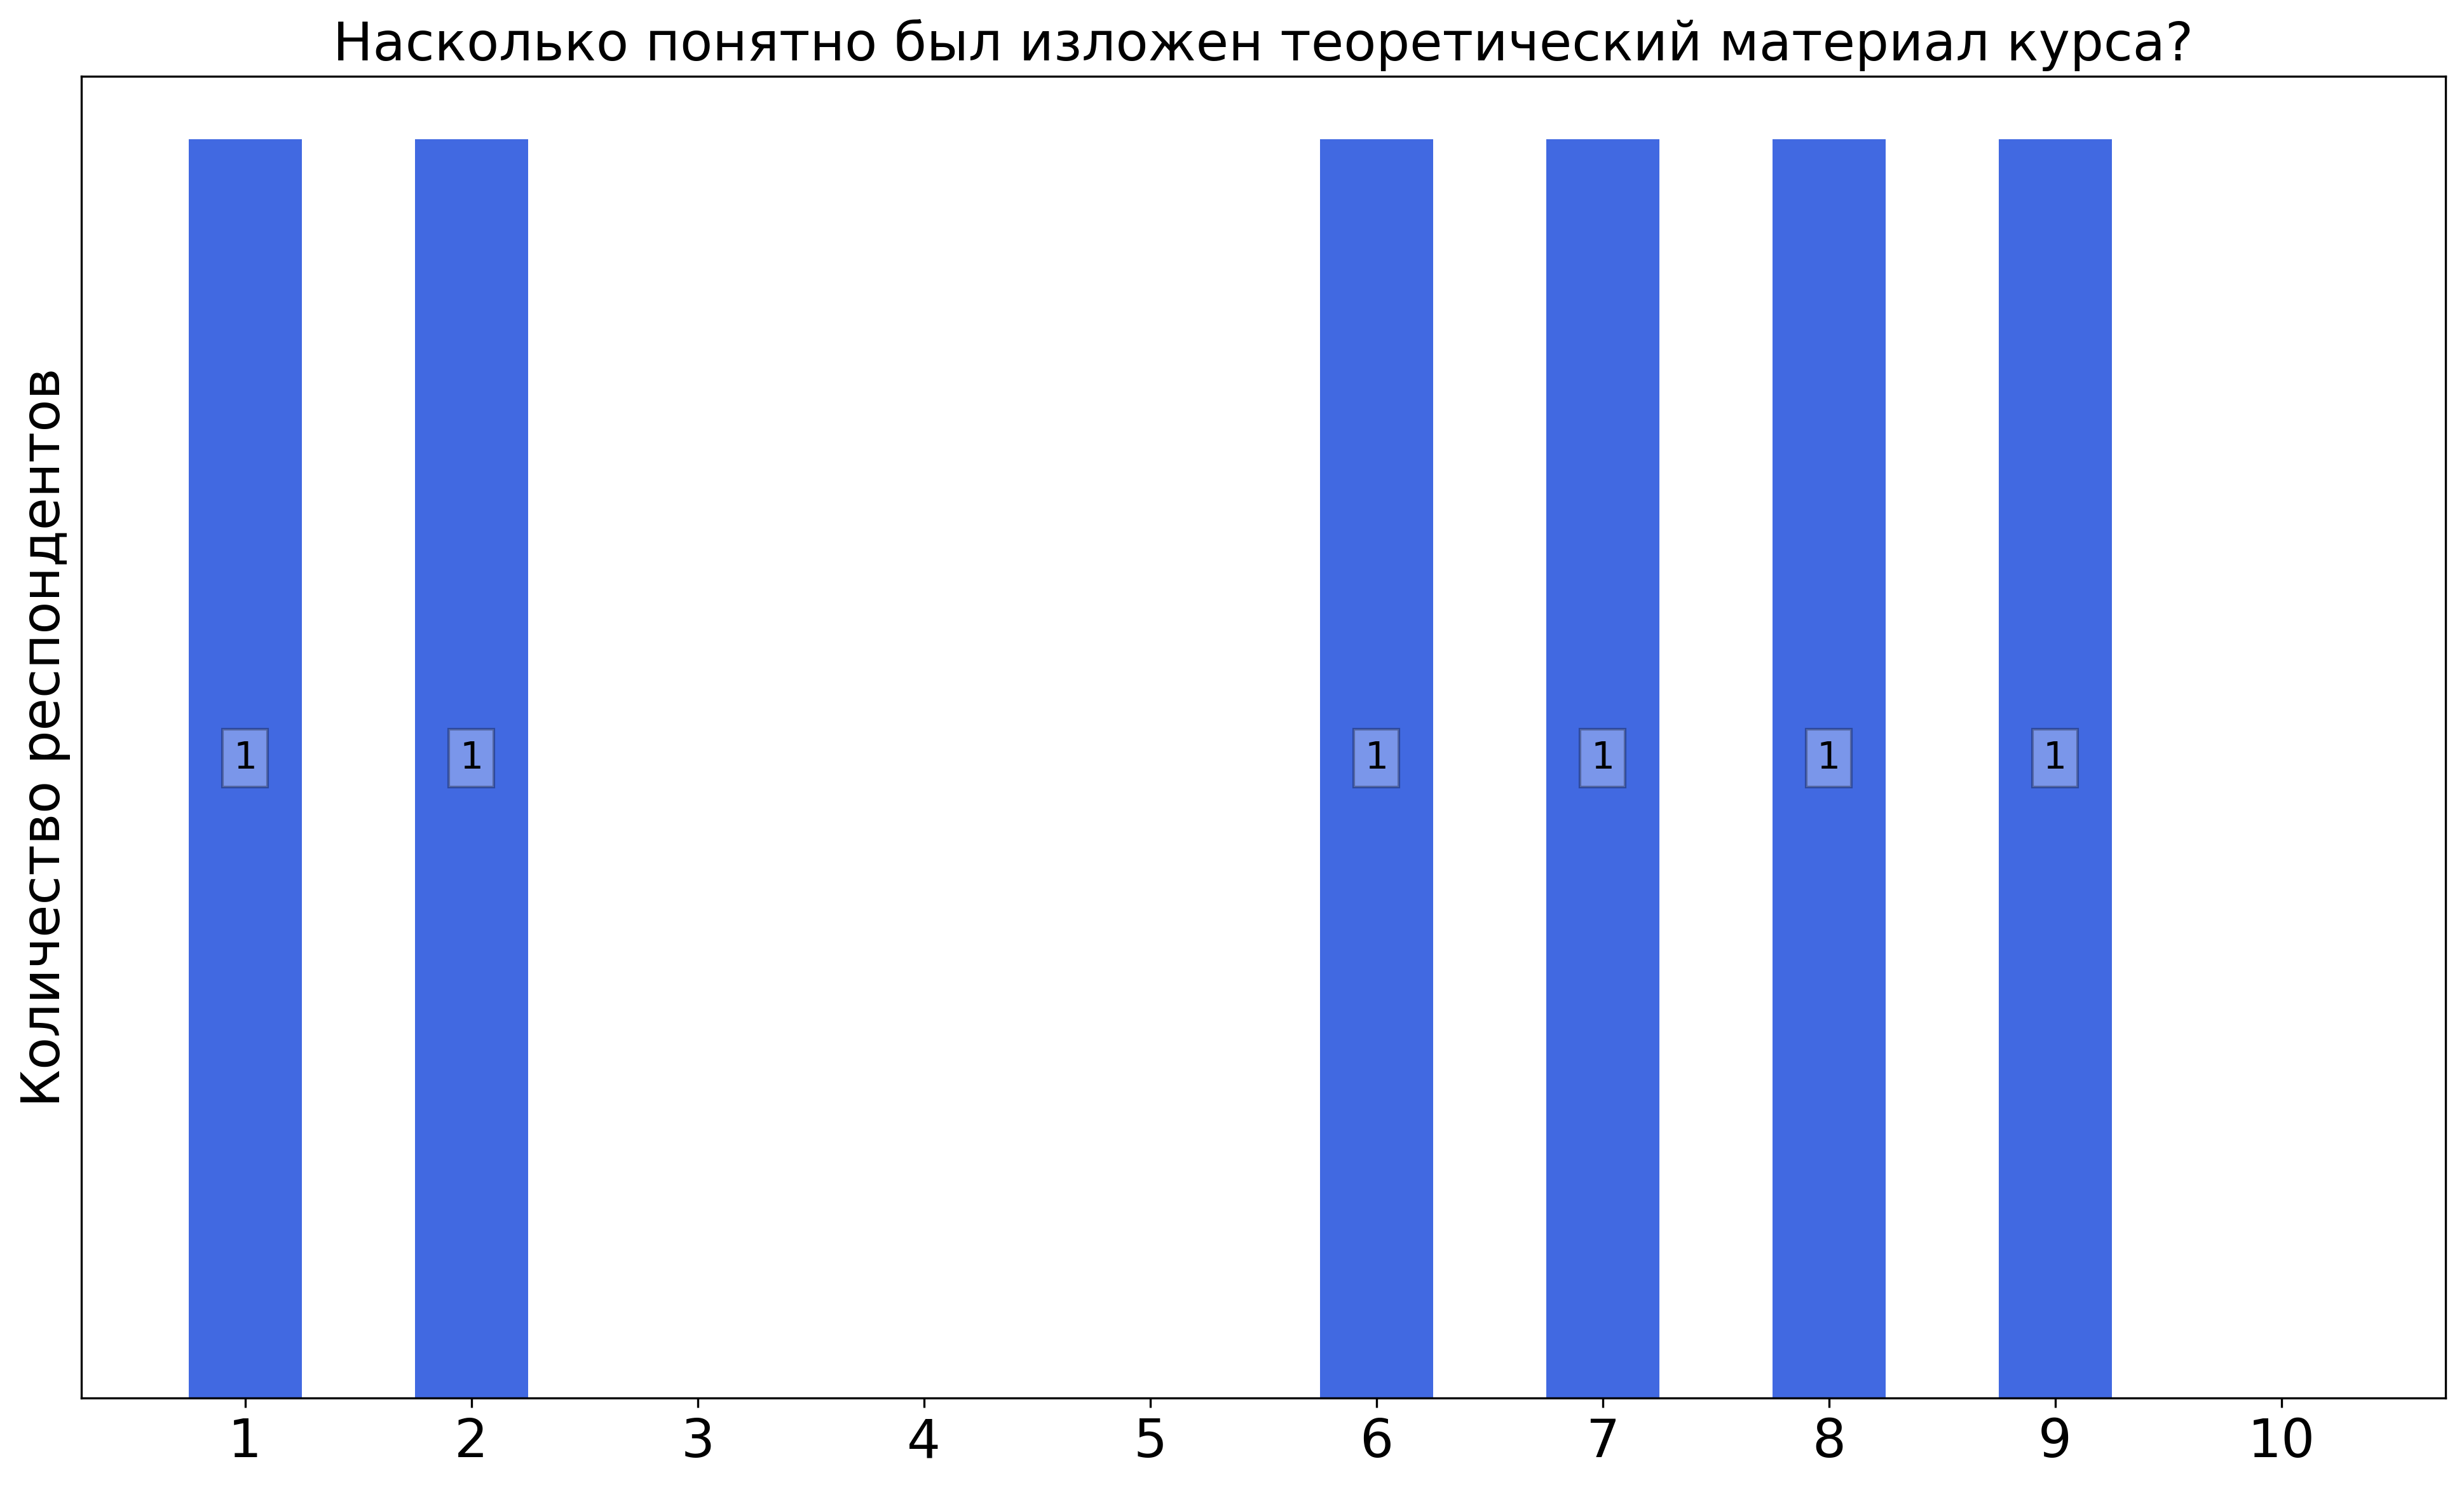
\includegraphics[width=\textwidth]{images/4 course/Введение в машинное обучение/lecturer-marks-Воронцов К.В.-2.png}
			\end{subfigure}	
			\begin{subfigure}[b]{0.45\textwidth}
				\centering
				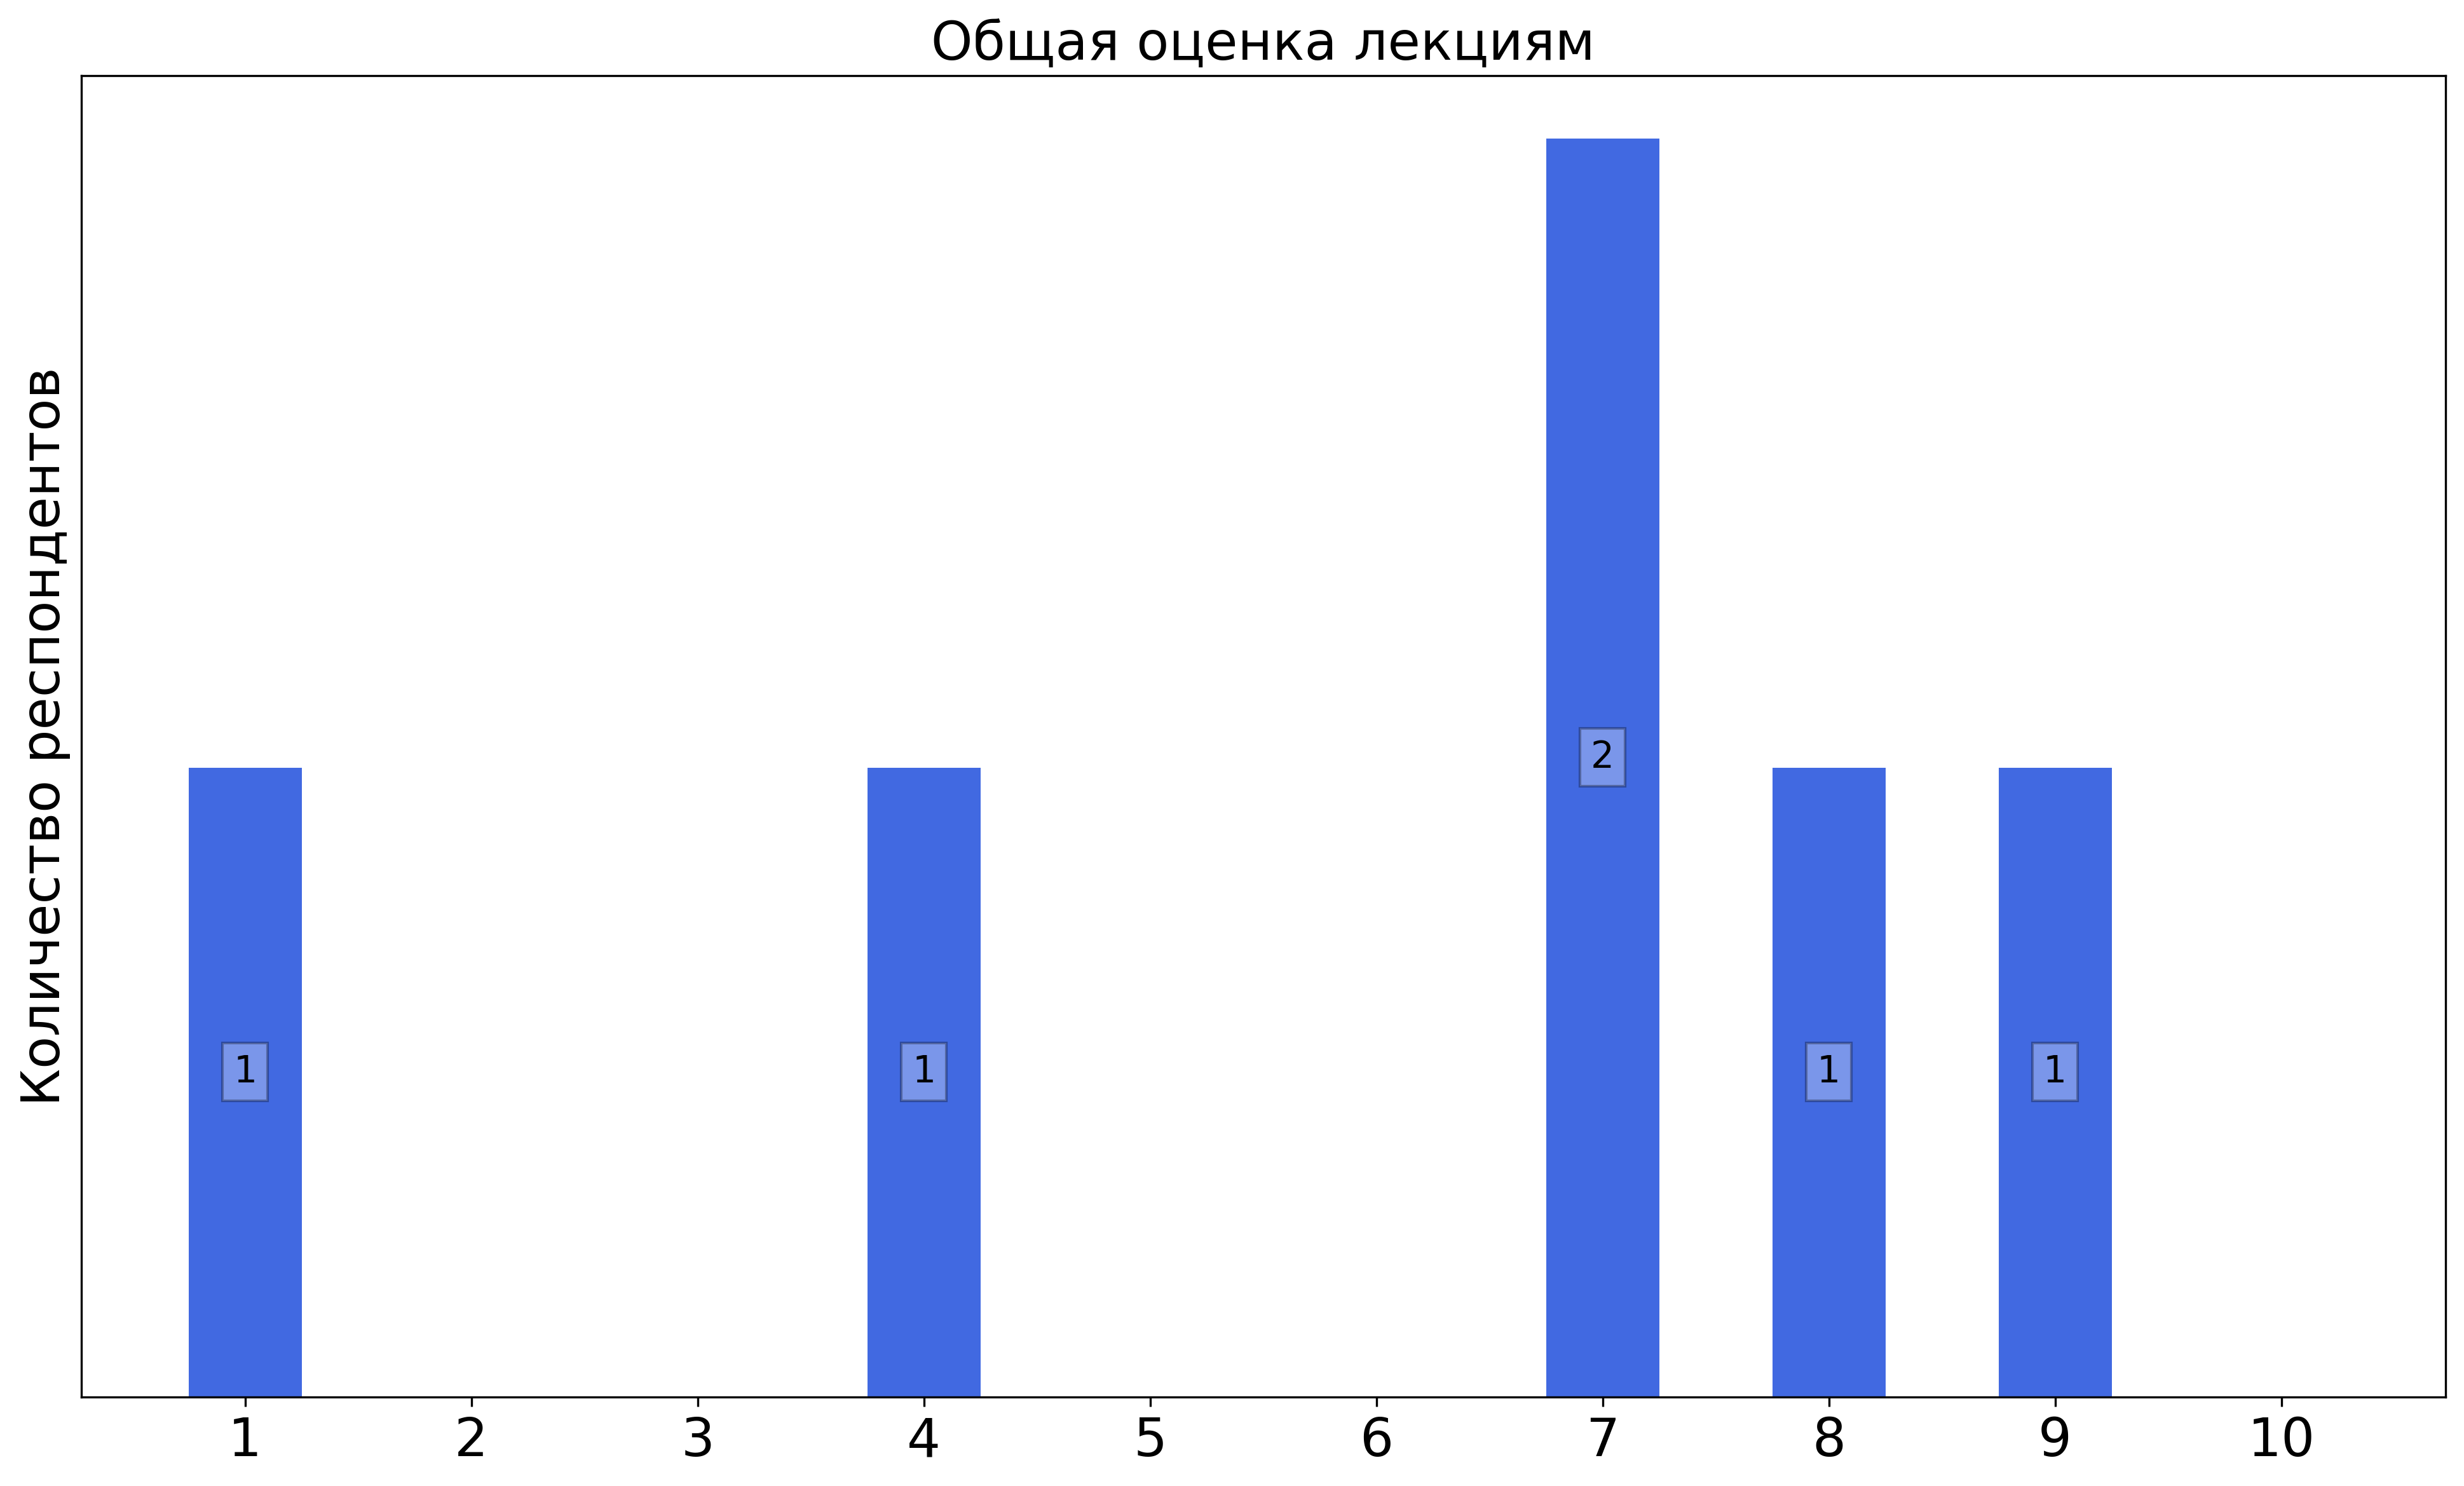
\includegraphics[width=\textwidth]{images/4 course/Введение в машинное обучение/lecturer-marks-Воронцов К.В.-3.png}
			\end{subfigure}
			\caption{Оценки респондентов о качестве преподавания лекций по курсу <<Введение в машинное обучение>>}
		\end{figure}

		\textbf{Комментарии студентов о лекциях\protect\footnote{сохранены оригинальные орфография и пунктуация}} 
            \begin{commentbox} 
                К лекциям готовится. Людей ходит много. Математика рассчитана не на РТ знания. 
                По вопросам не знаешь особо что и задать. Но он в основном просто читает, не отвечает особо 
            \end{commentbox}


    \subsubsection{Отзыв студентов о лекциях. Лектор: Нейчев Р.Г.}
		\begin{figure}[H]
			\centering
            \begin{subfigure}[b]{0.45\textwidth}
				\centering
				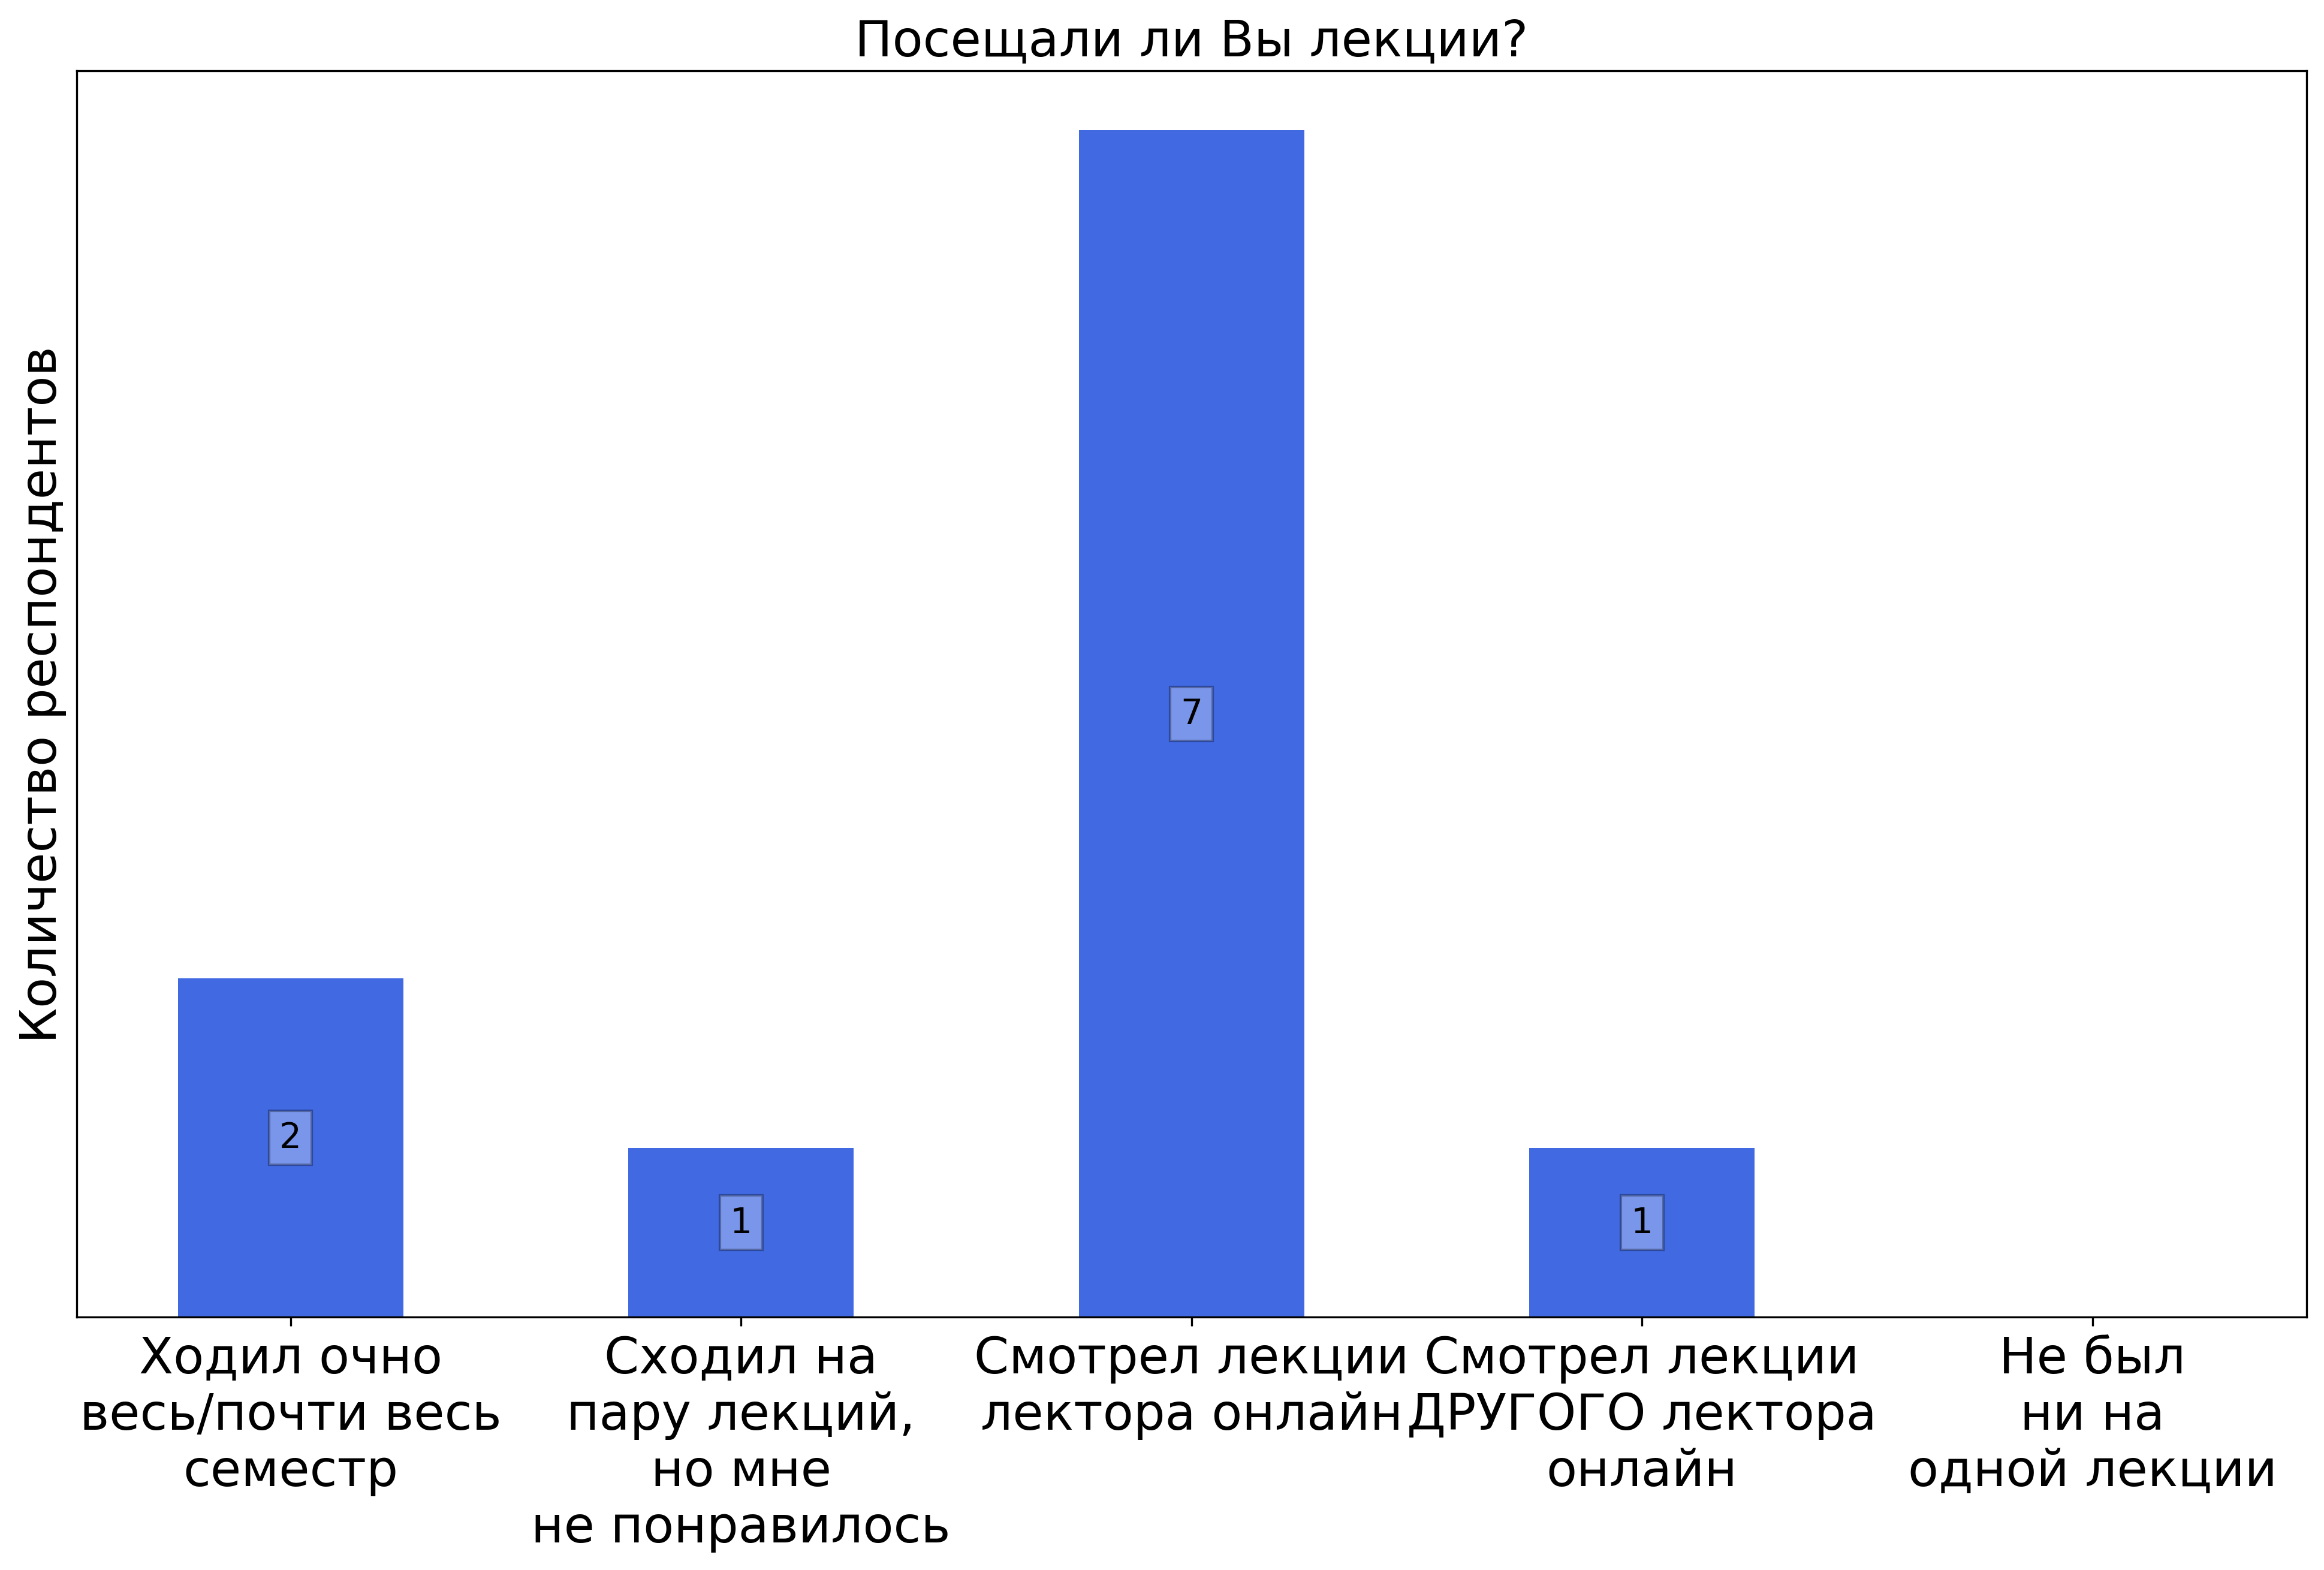
\includegraphics[width=\textwidth]{images/4 course/Введение в машинное обучение/lecturer-questions-Нейчев Р.Г.-0.png}
			\end{subfigure}
			\begin{subfigure}[b]{0.45\textwidth}
				\centering
				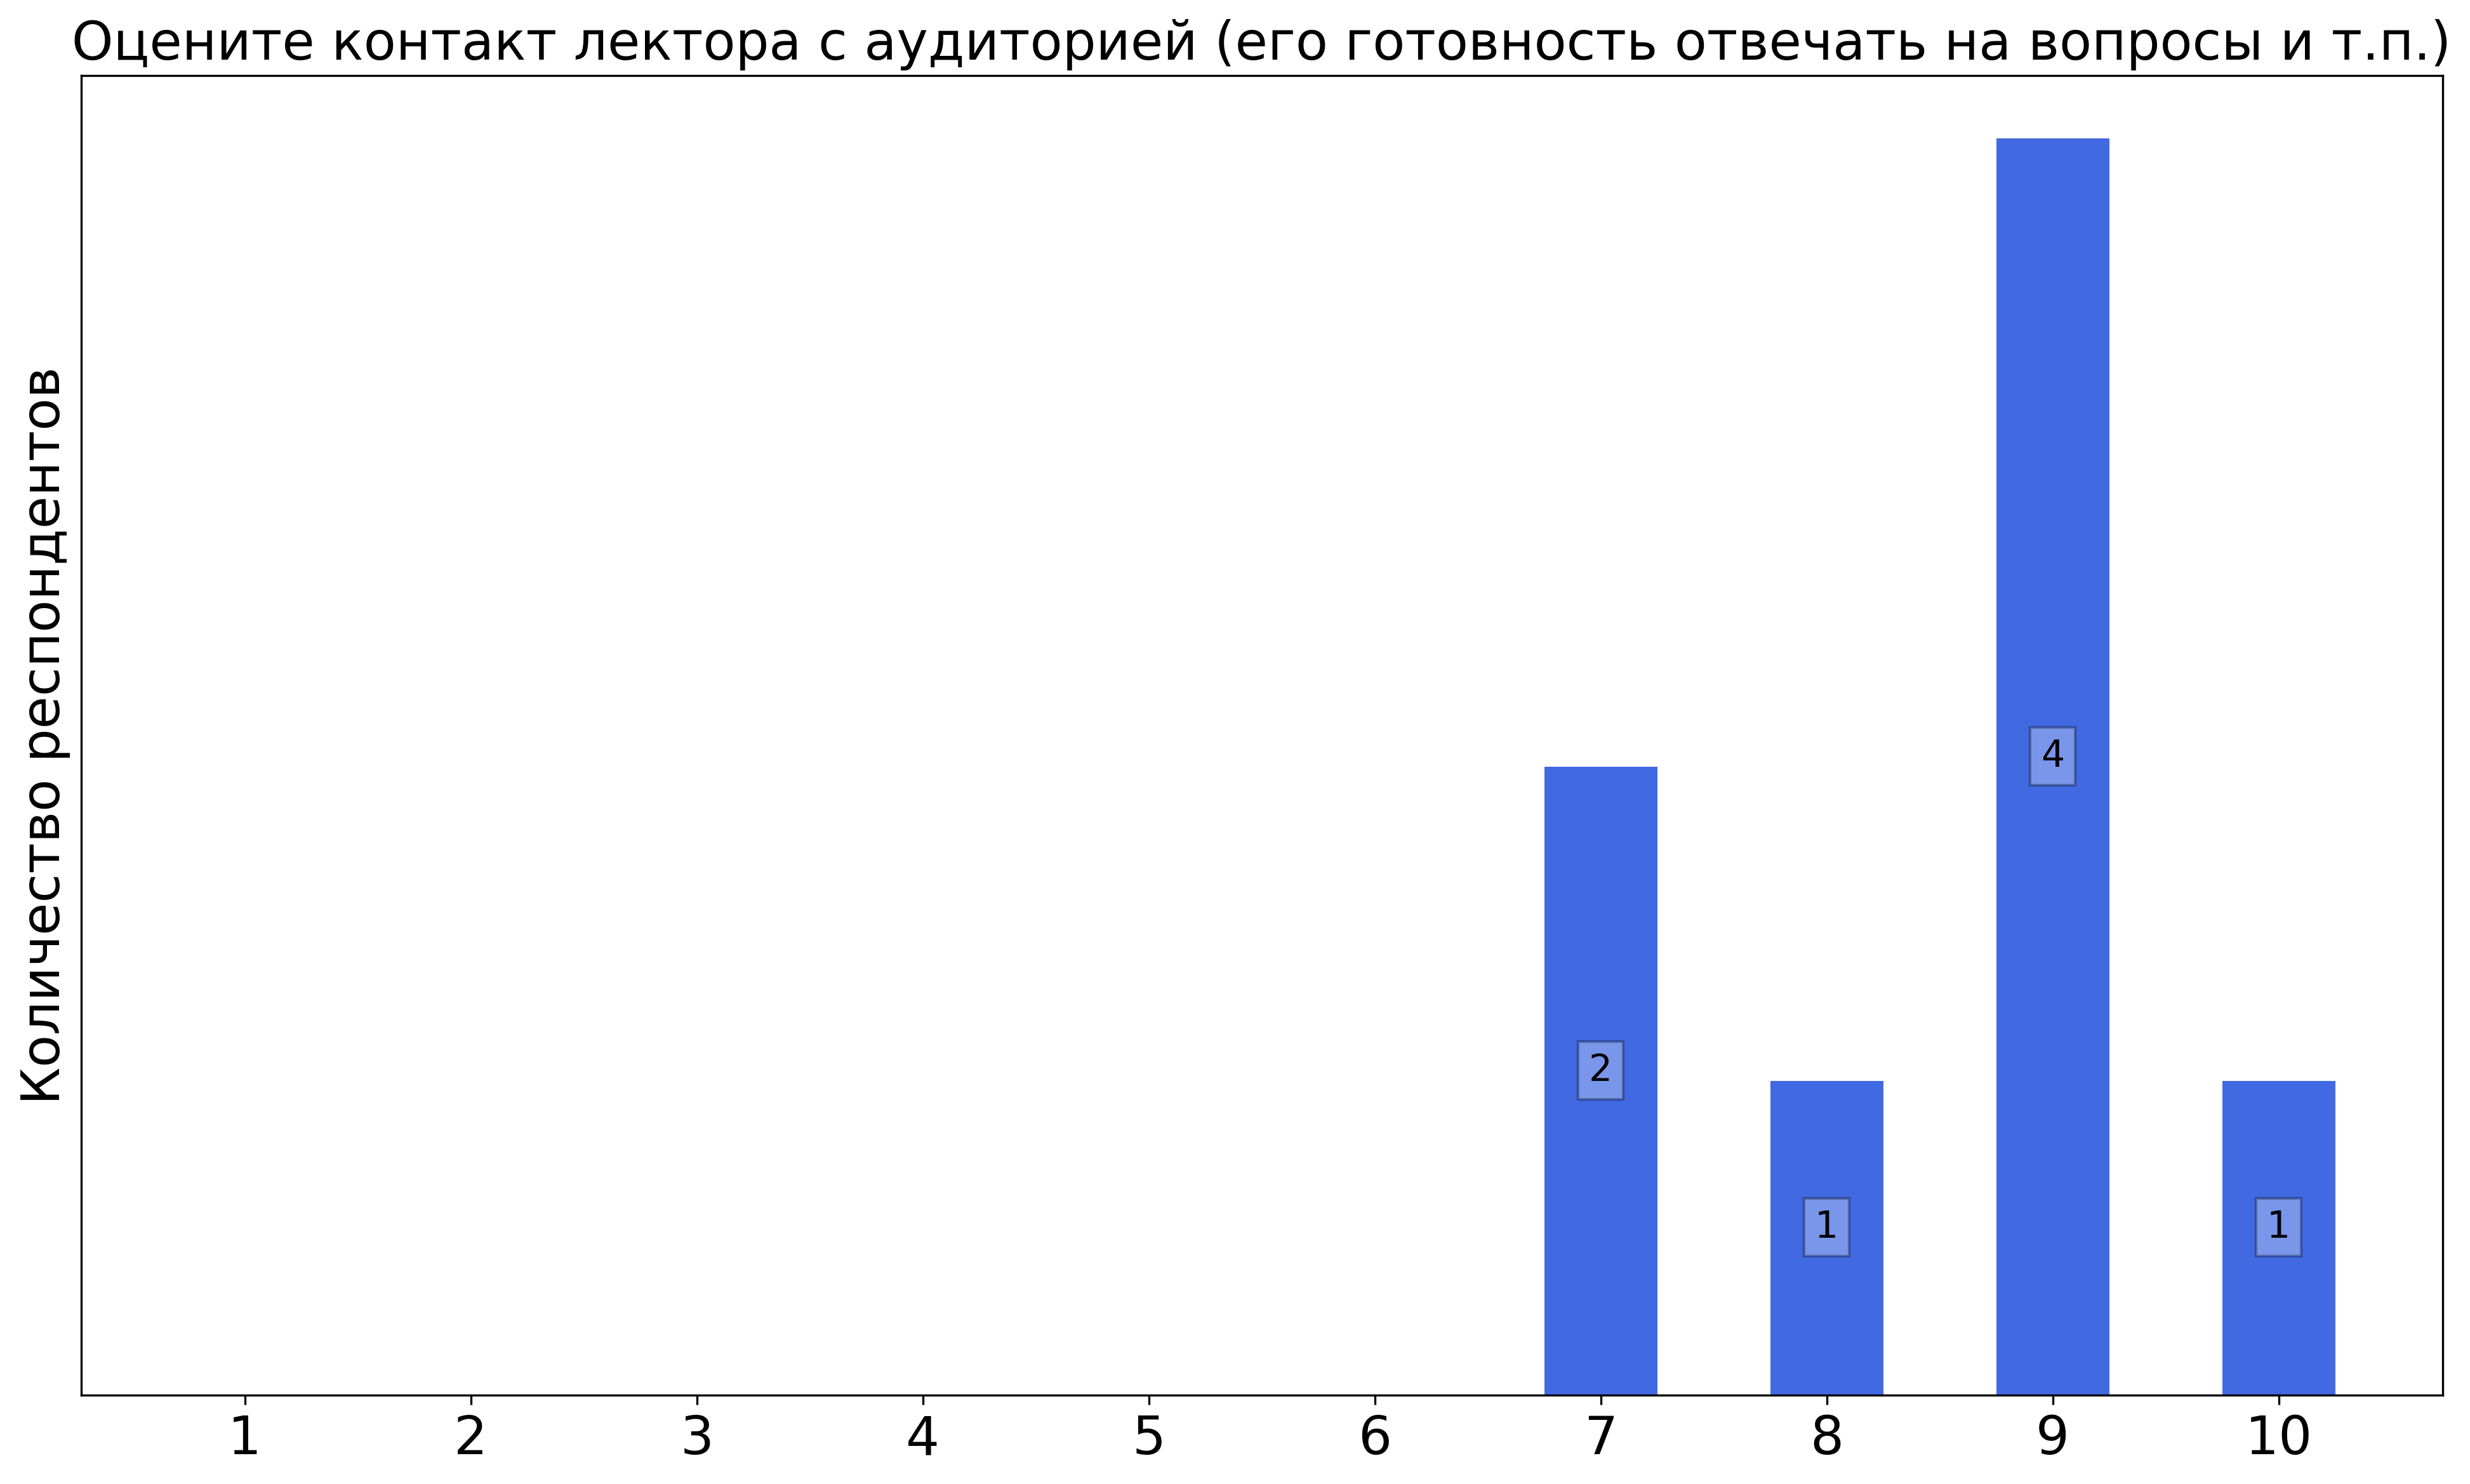
\includegraphics[width=\textwidth]{images/4 course/Введение в машинное обучение/lecturer-marks-Нейчев Р.Г.-0.png}
			\end{subfigure}
			\begin{subfigure}[b]{0.45\textwidth}
				\centering
				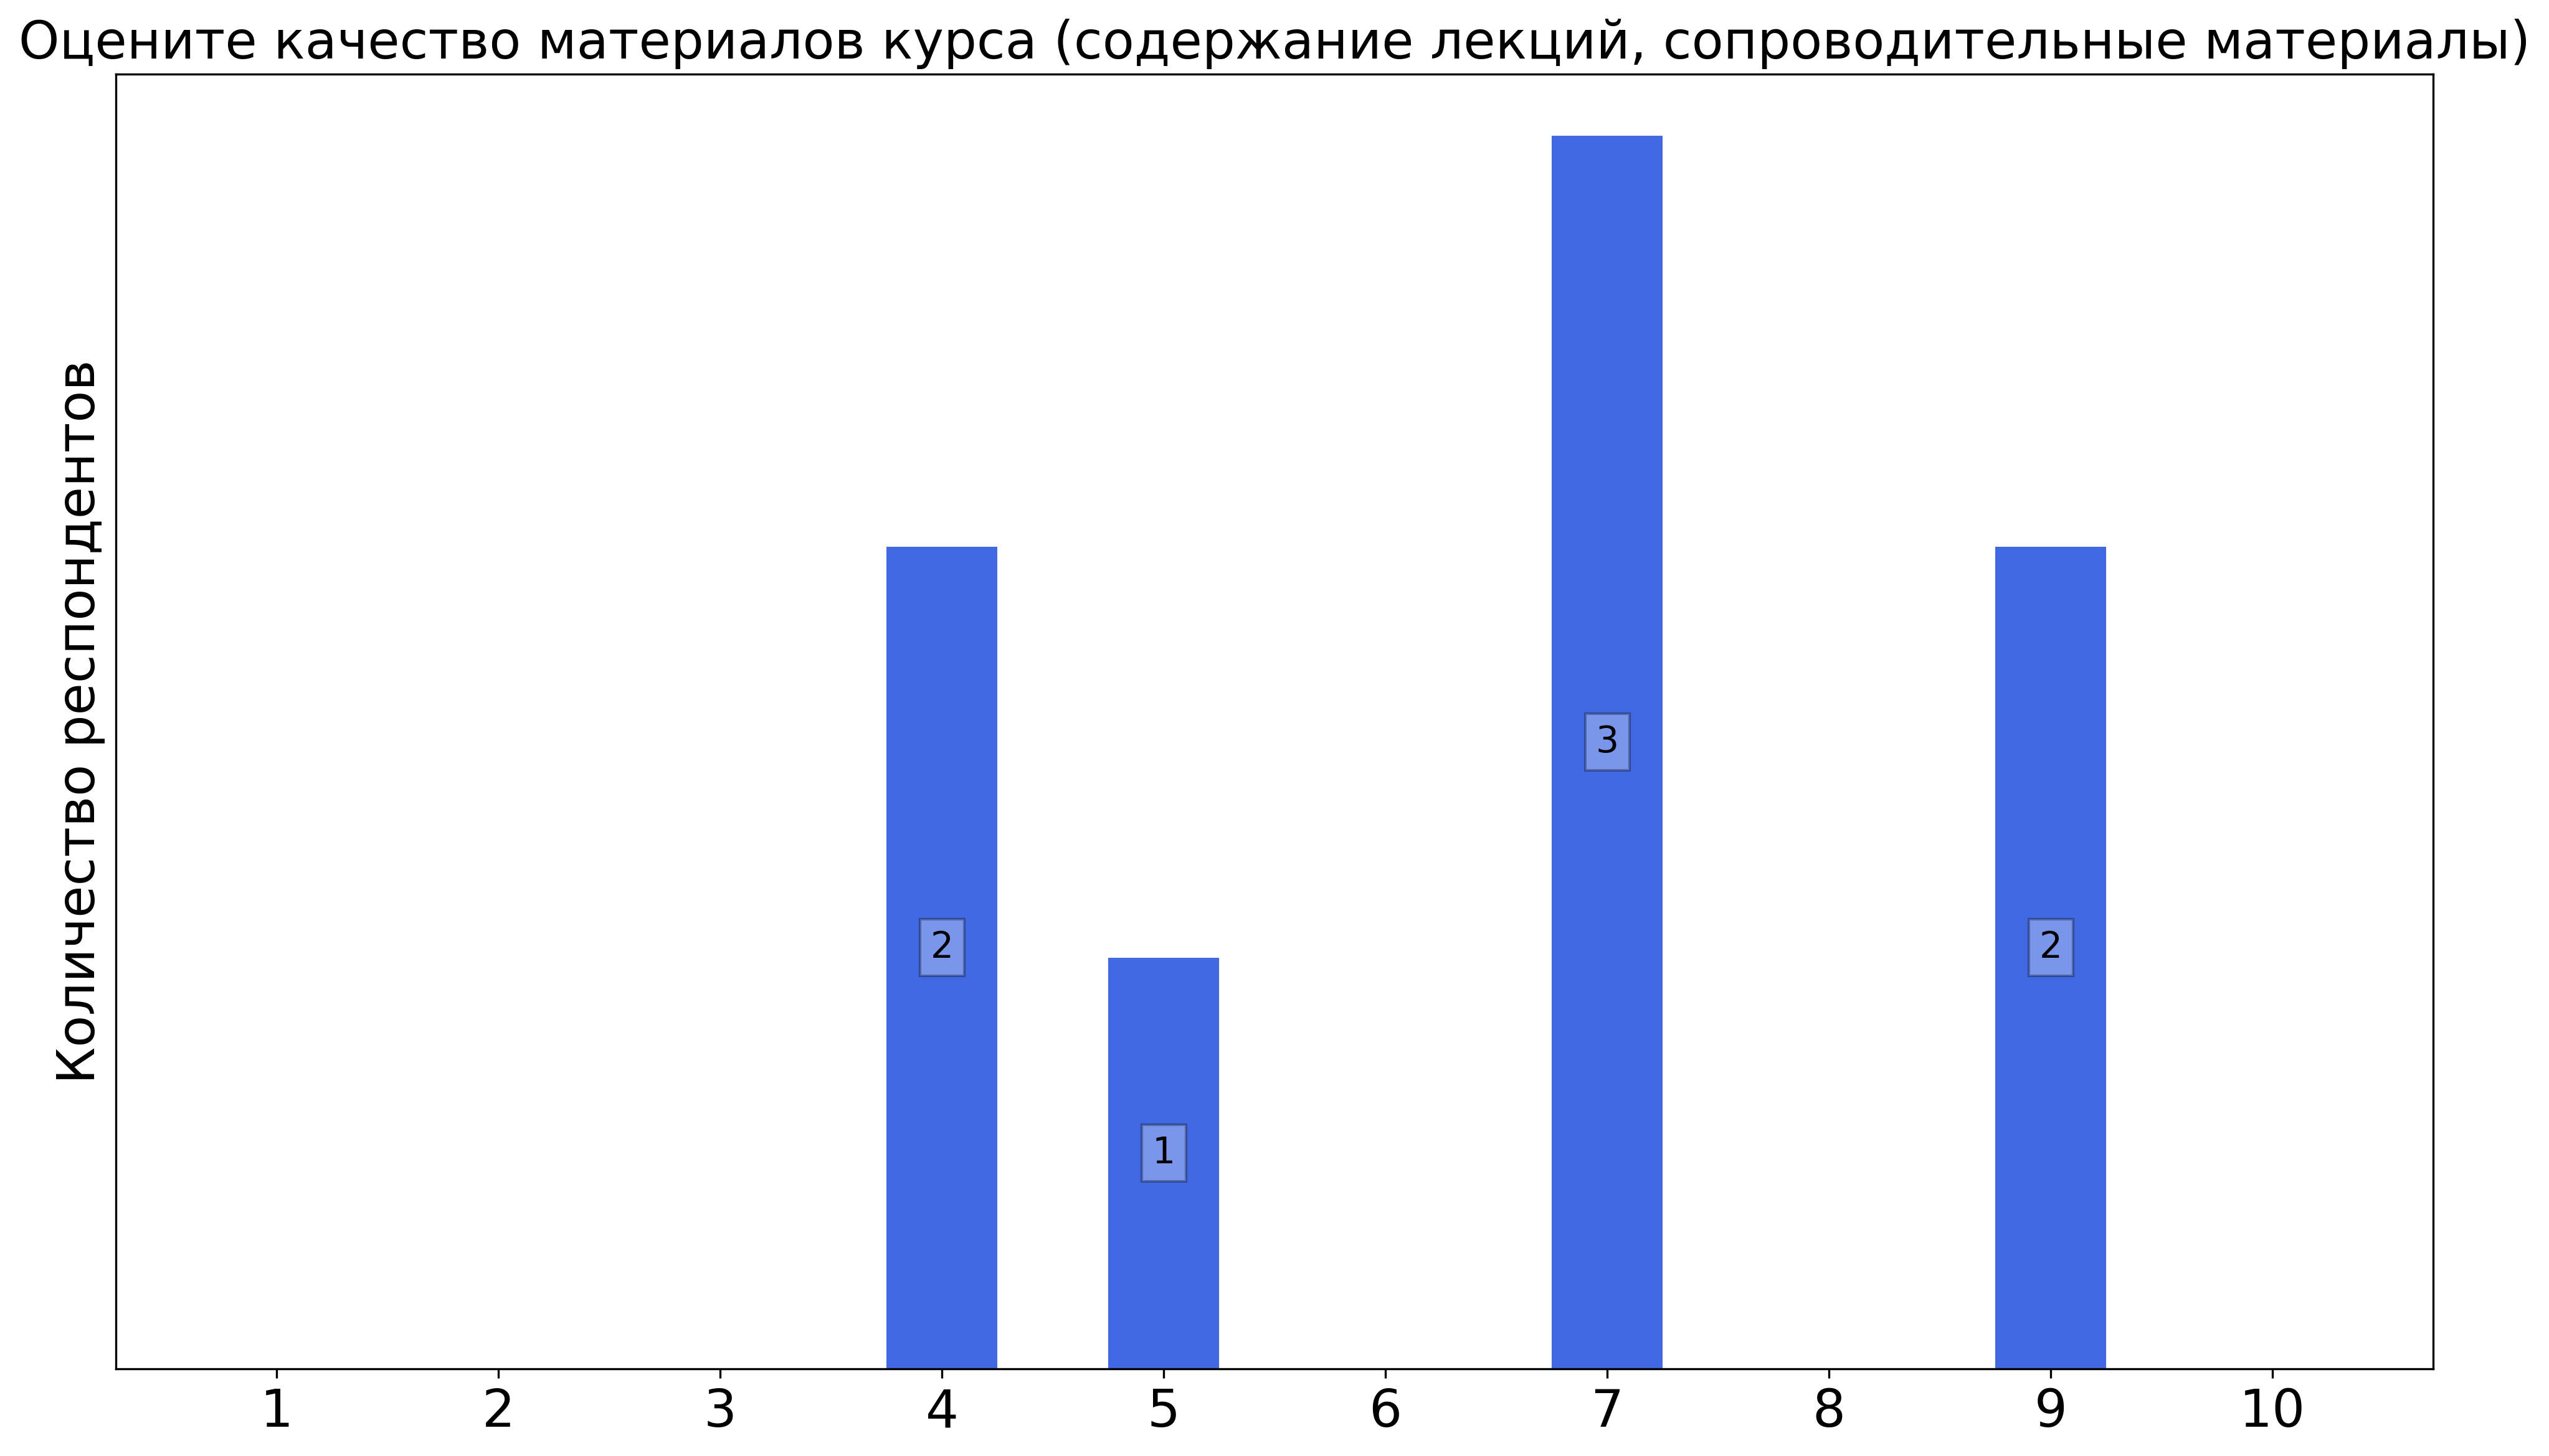
\includegraphics[width=\textwidth]{images/4 course/Введение в машинное обучение/lecturer-marks-Нейчев Р.Г.-1.png}
			\end{subfigure}
			\begin{subfigure}[b]{0.45\textwidth}
				\centering
				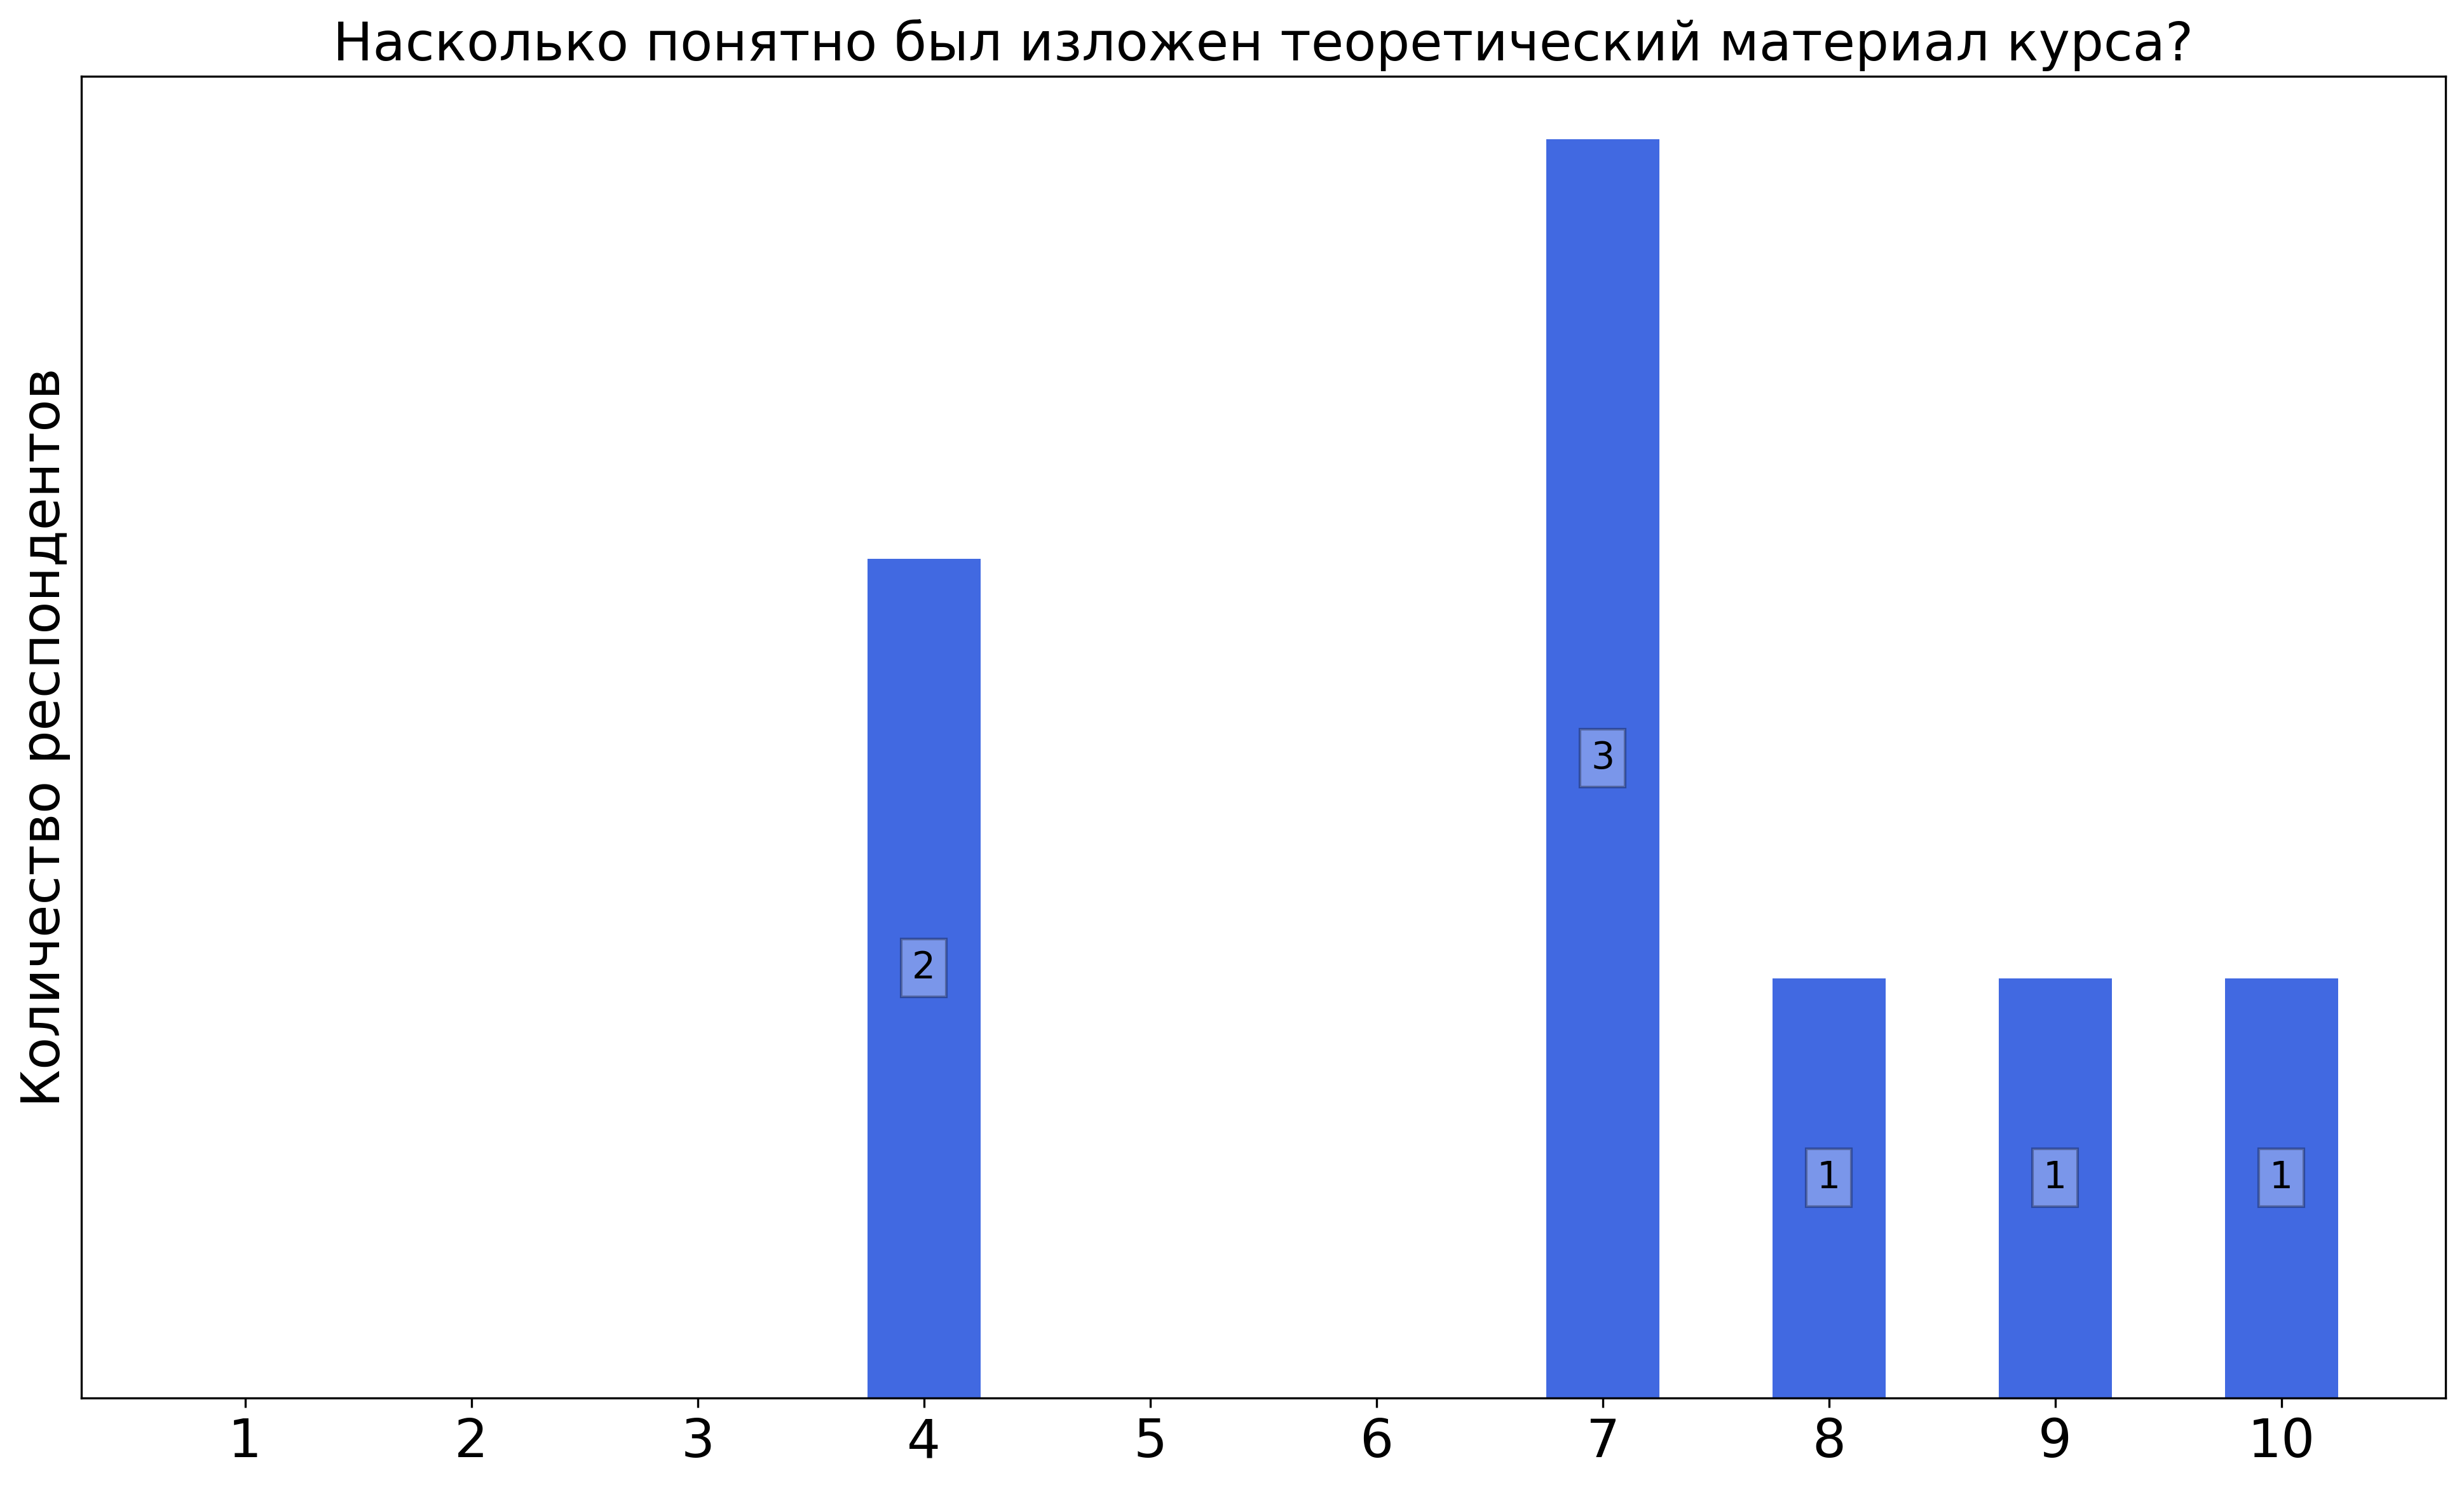
\includegraphics[width=\textwidth]{images/4 course/Введение в машинное обучение/lecturer-marks-Нейчев Р.Г.-2.png}
			\end{subfigure}	
			\begin{subfigure}[b]{0.45\textwidth}
				\centering
				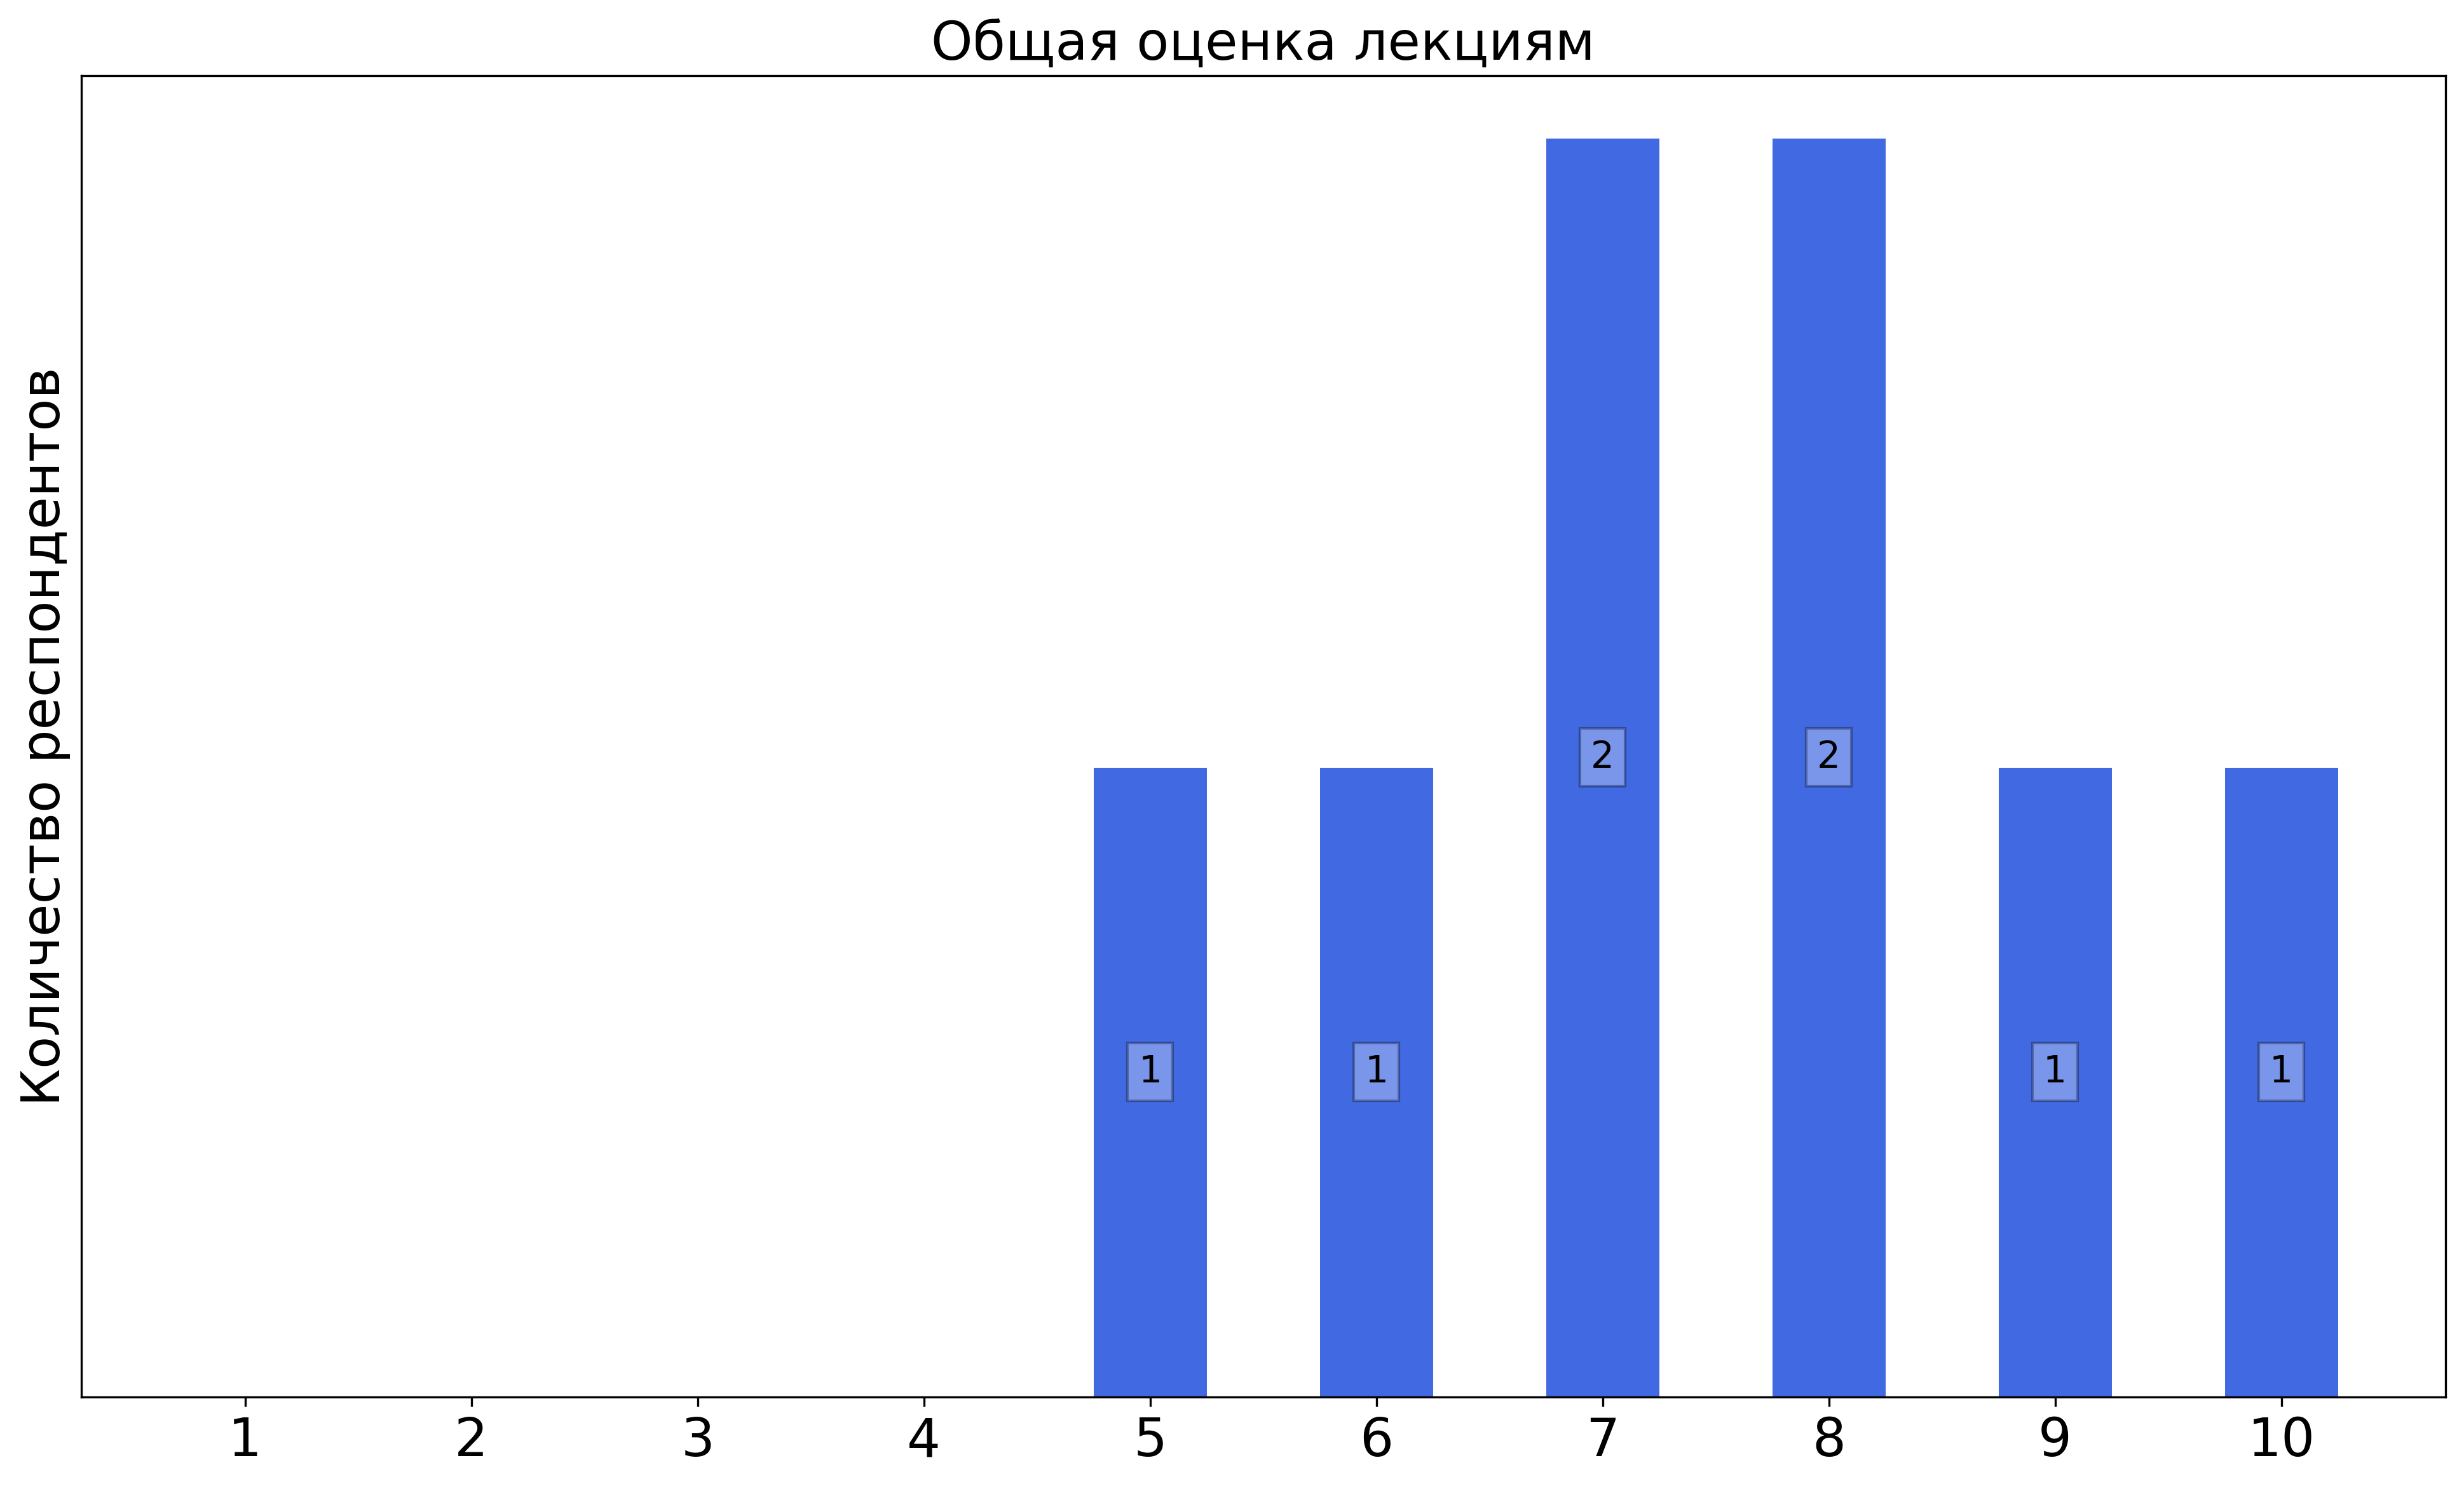
\includegraphics[width=\textwidth]{images/4 course/Введение в машинное обучение/lecturer-marks-Нейчев Р.Г.-3.png}
			\end{subfigure}
			\caption{Оценки респондентов о качестве преподавания лекций по курсу <<Введение в машинное обучение>>}
		\end{figure}

		\textbf{Комментарии студентов о лекциях\protect\footnote{сохранены оригинальные орфография и пунктуация}}
            \begin{commentbox} 
                Лекции сильно опираются на курсы статистики и методов оптимизации, что логично и понятно без этого никак. Но на потоке РТ, где их не было, смотрится тяжело. Соответственно вопрос зачем на РТ вообще машинка и если её ставить, то тогда вопрос где предварительное ознакомление с вышеуказанными предметами. Аргумент в духе "вся литература по этой части была указана в курсе лекций, при желании можно ознакомиться" даже не имеет смысла, его можно припихнуть ко всему и давать машинку на 1м курсе
            \end{commentbox} 
        
            \begin{commentbox} 
                Всё очень понравилось. Лектор постоянно взаимодействовал с аудиторией, активно отвечал на все вопросы. При необходимости поправлял, дообъяснял, проводил дискуссии. Так, после лекций, при желании можно ответить на все волнующие себя вопросы 
            \end{commentbox} 
        
            \begin{commentbox} 
                1. Плохая организация курса: лабораторные работы не были проверены до самого экзамена; на экзамене преподаватели не впускали в аудиторию в свое время (столкнулась с такой ситуацией впервые), студенты которые должны были заходить со мной минимум час ждали в коридоре чтобы нас взяли на экзамен и потом еще ожидали чтоб у нас начали принимать экзамен.
                2. Частые ошибки на слайдах которые использовались в лекциях
                3. Там два преподавателя лекций и они очень по разному подают материал. Мне показалось что часть вещей разбирались довольно поверхностно (например причинно-следственные связи в каких то фактах, которые потом спросят на экзамене или в теоремах)
                4. Большим минусом на мой взгляд оказалось что до самого экзамена не были ясны критерии оценки, не было четко сказано как именно будут влиять сданные лабораторки (по итогу так и не поняла повлияли ли они). С организацией проблемы: не было сообщено о дне экзамена, в день официального зачета у нашего потока мы так и не знали дату когда можем прийти на экзамен чтоб закрыть курс. Четкой программы по которой спрашивают преподы на экзамене нет. Вопросы из головы, я считаю это ведет к тому что у преподавателей большая степень свободы и соответственно меньшая объективность. И готовиться это мешает + материалы которые я видела не слишком полные и неофициальные - я пользовалась конспектами лекций но они от студентов и много что там упущено и не объяснено.
            \end{commentbox} 
        
            \begin{commentbox} 
                Оба лектора и семинариста рассказывают нормально, конспекты прям топ. 
            \end{commentbox} 
    
    
    \subsubsection{Отзыв студентов о семинарах. Семинарист: Грабовой А.}
		\begin{figure}[H]
			\centering
			\begin{subfigure}[b]{0.45\textwidth}
				\centering
				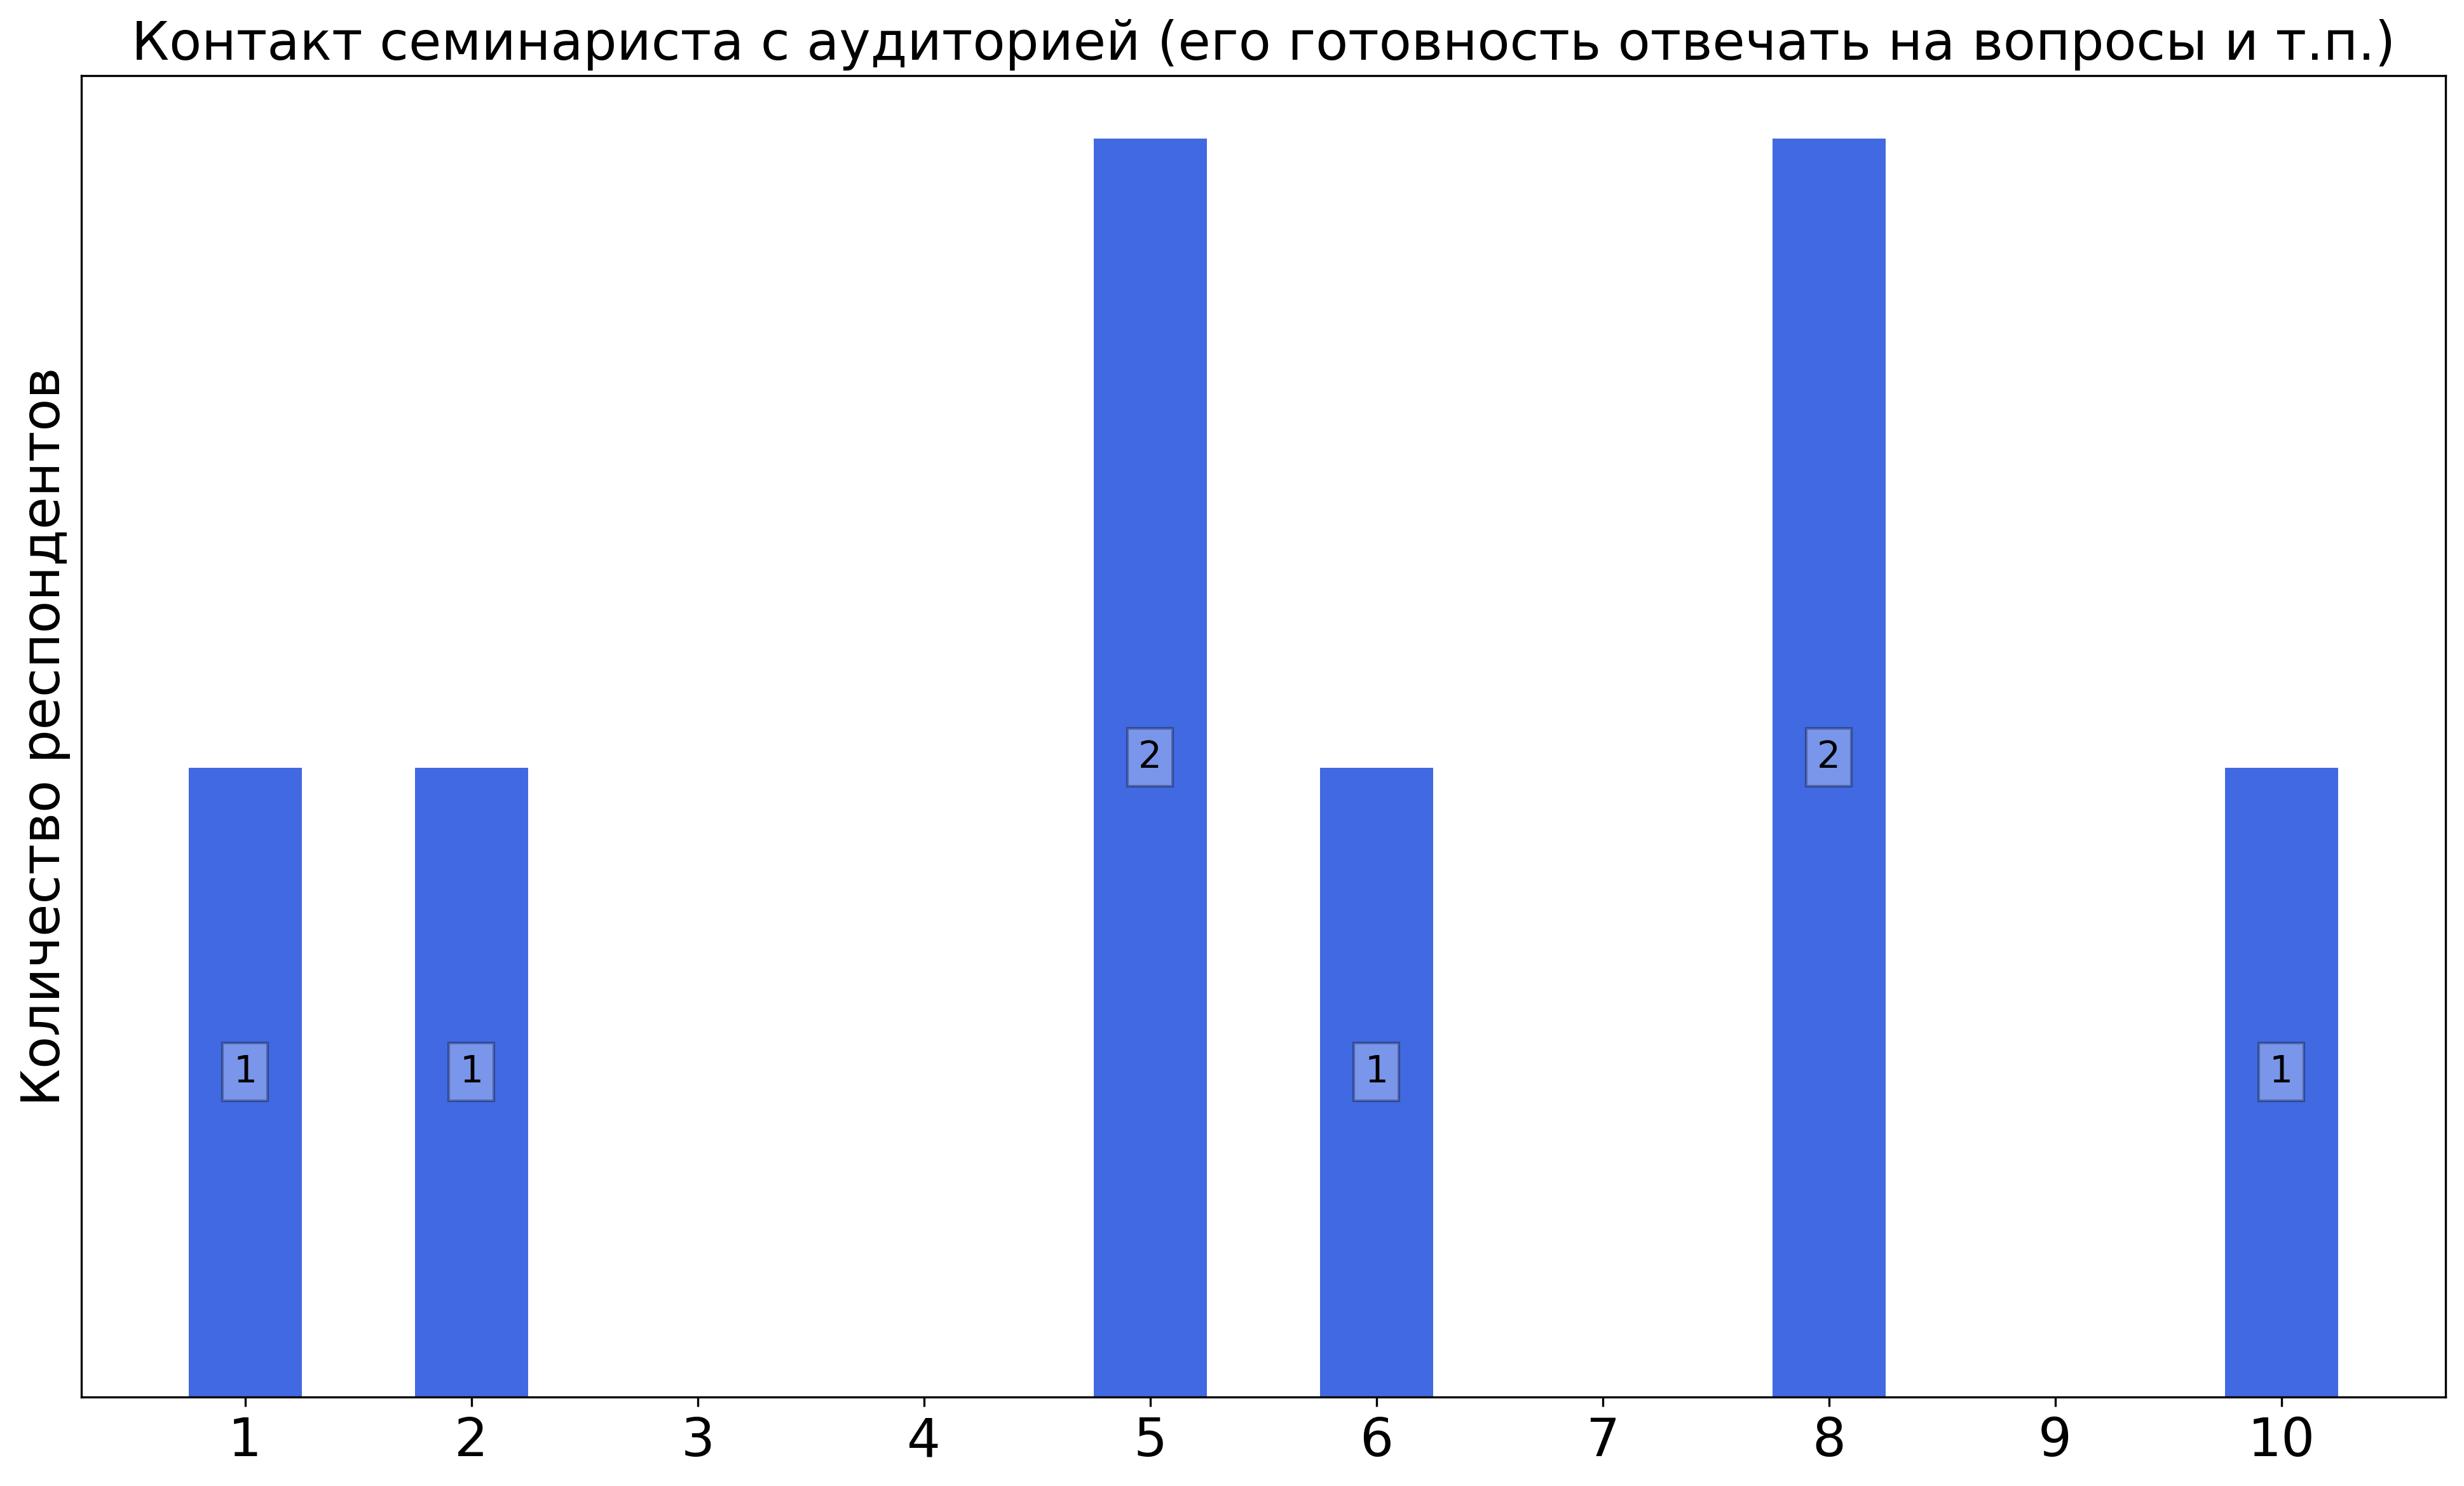
\includegraphics[width=\textwidth]{images/4 course/Введение в машинное обучение/seminarists-marks-Грабовой А.-0.png}
			\end{subfigure}
			\begin{subfigure}[b]{0.45\textwidth}
				\centering
				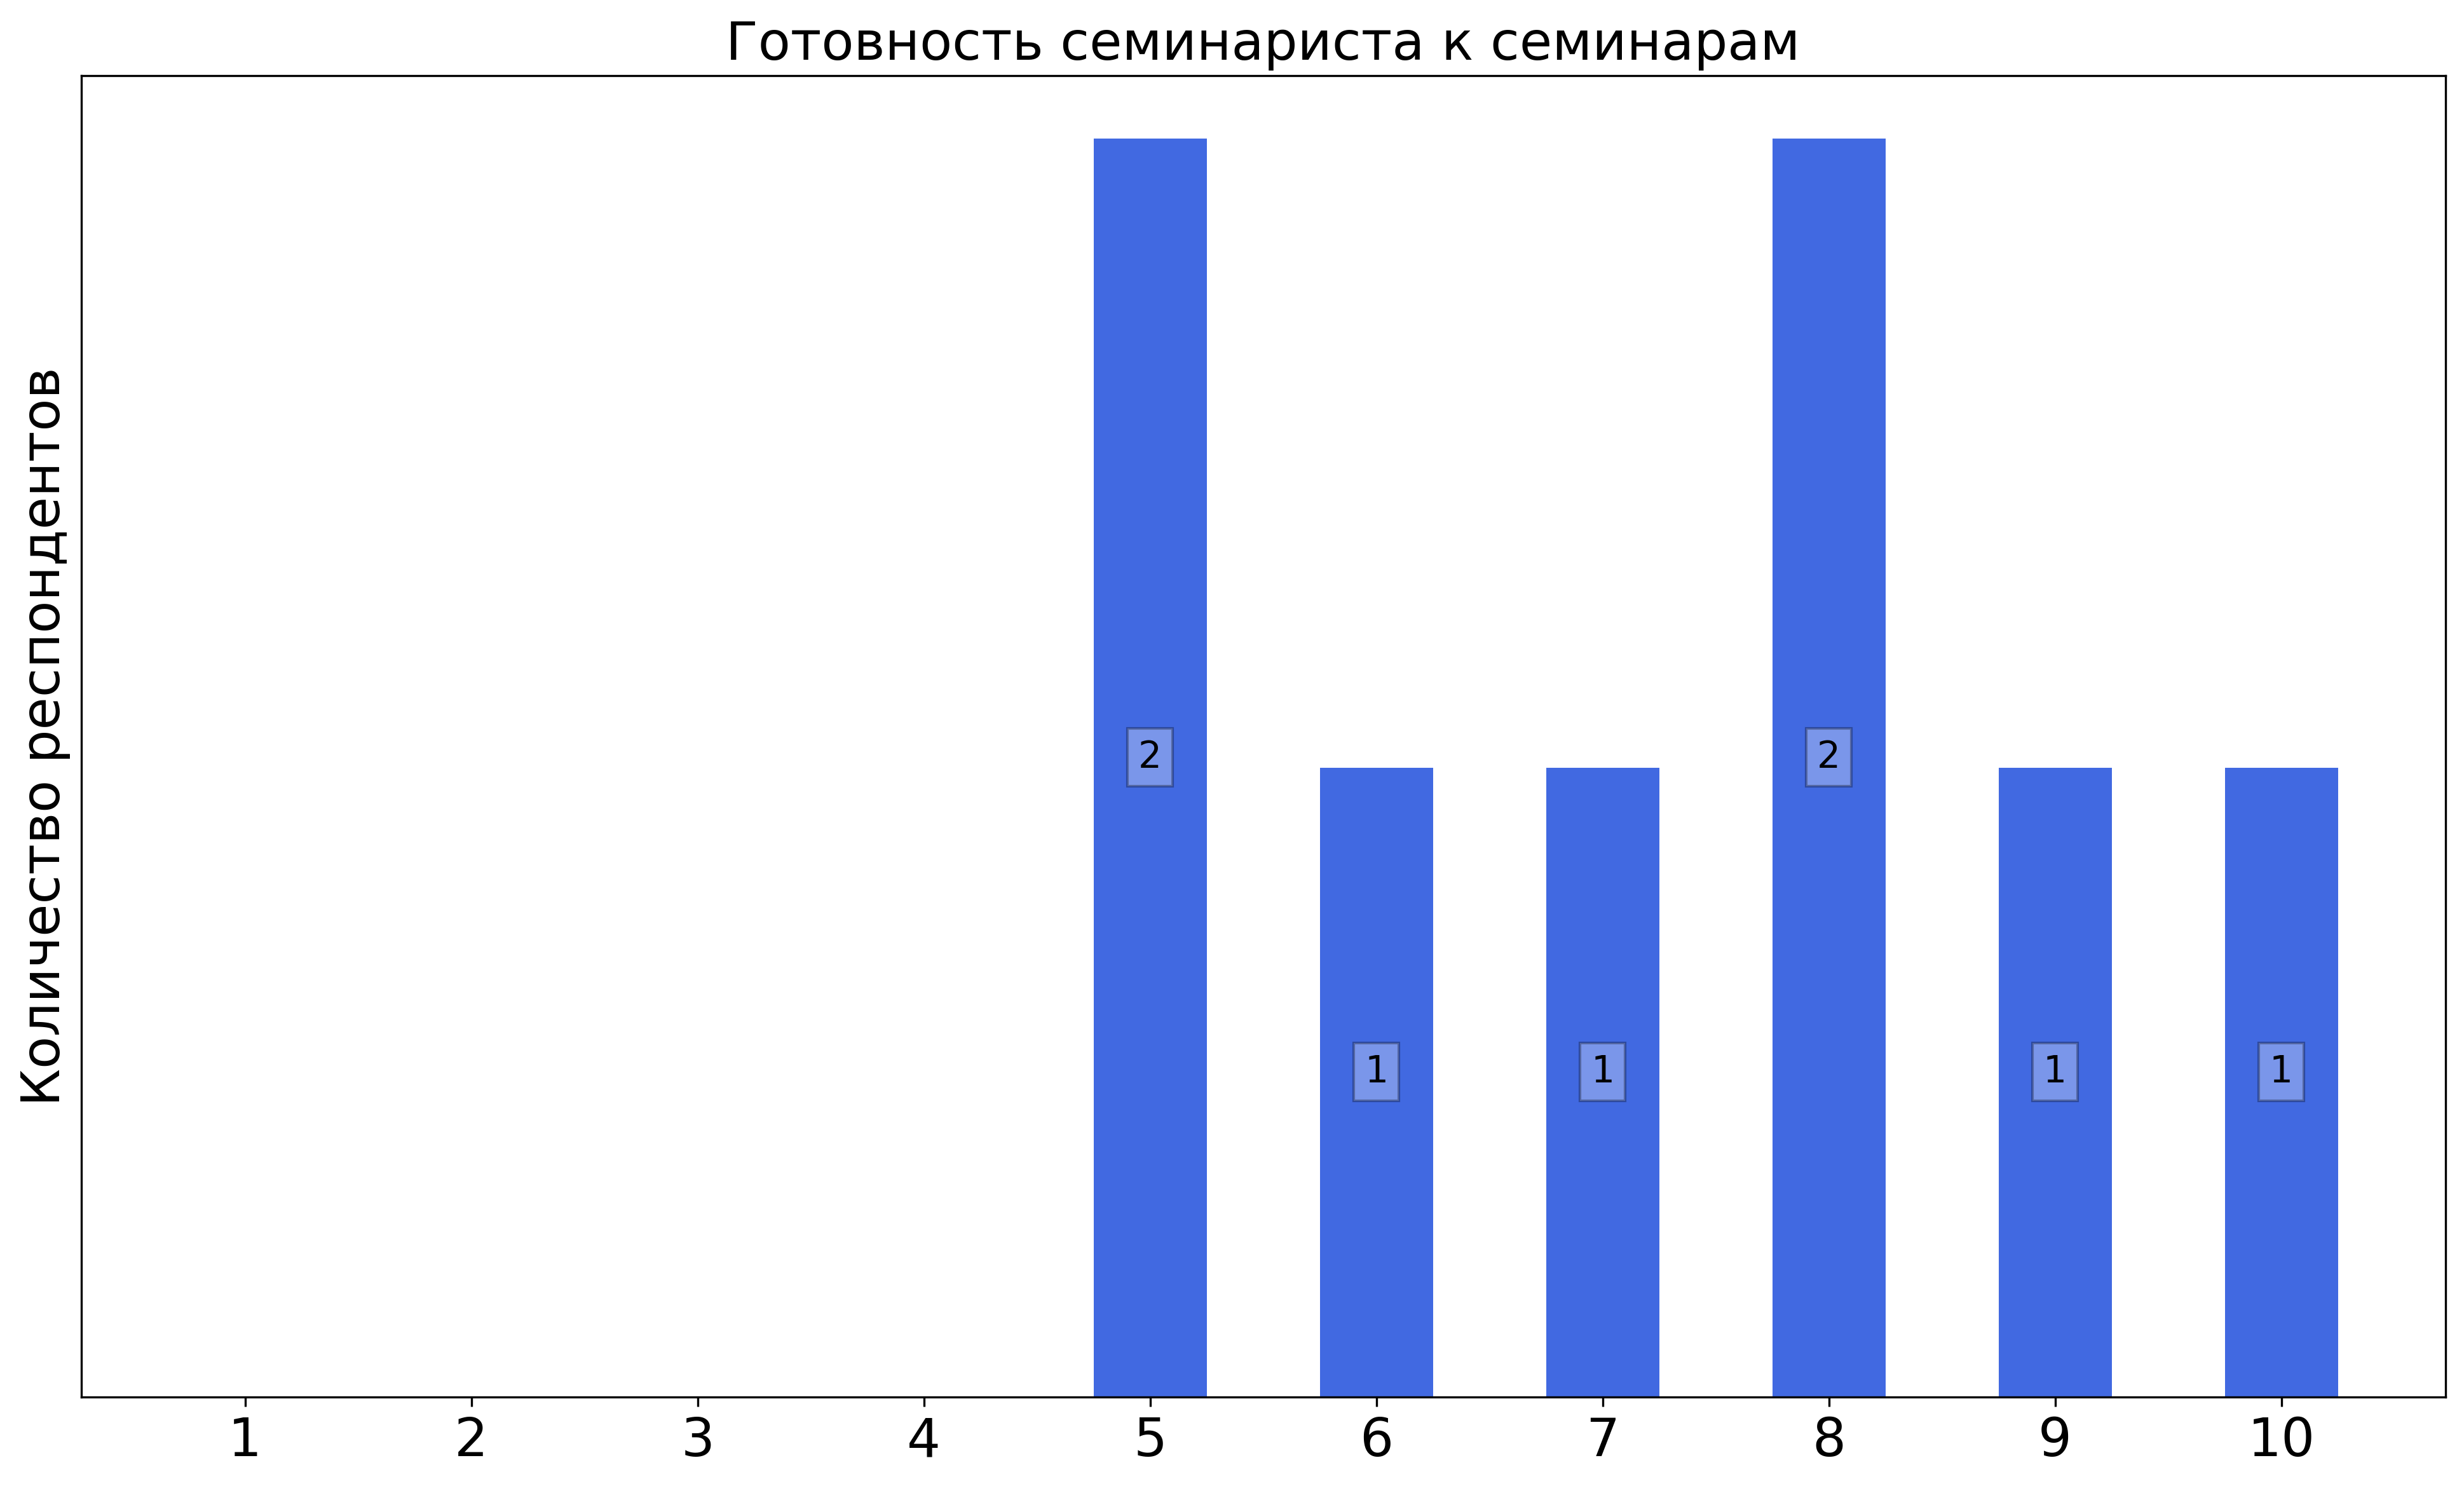
\includegraphics[width=\textwidth]{images/4 course/Введение в машинное обучение/seminarists-marks-Грабовой А.-1.png}
			\end{subfigure}
			\begin{subfigure}[b]{0.45\textwidth}
				\centering
				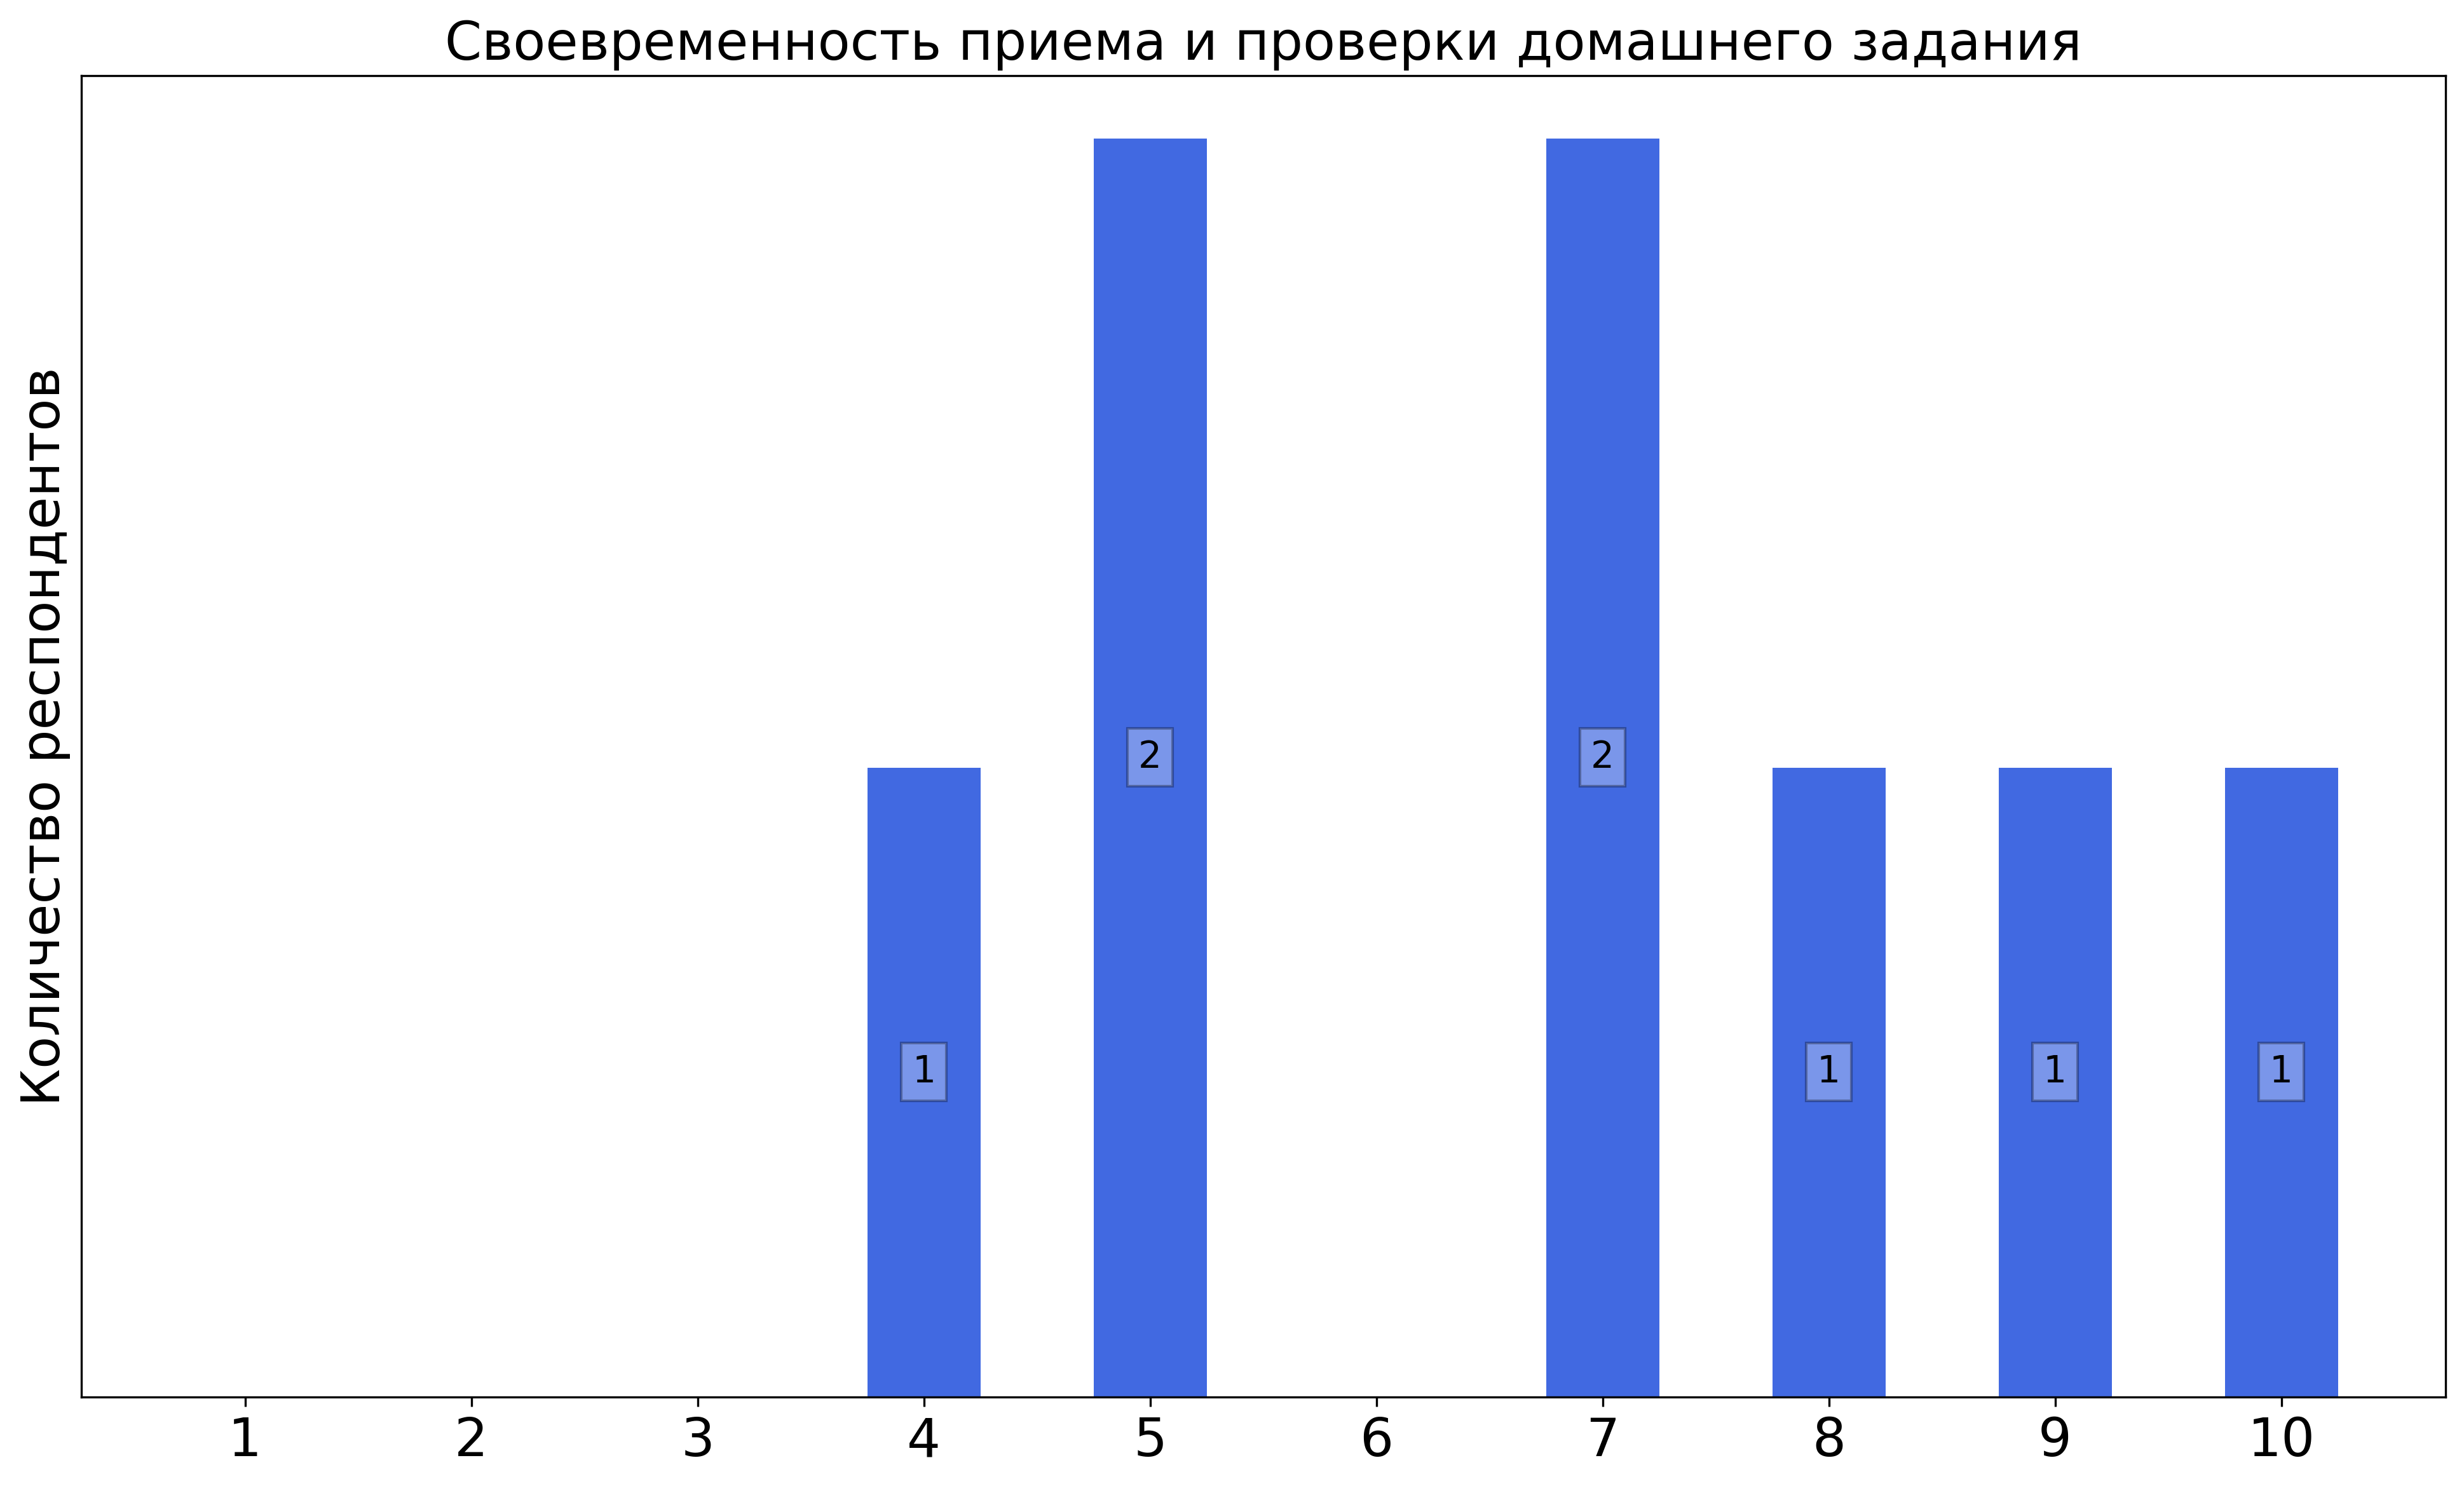
\includegraphics[width=\textwidth]{images/4 course/Введение в машинное обучение/seminarists-marks-Грабовой А.-2.png}
			\end{subfigure}
			\begin{subfigure}[b]{0.45\textwidth}
				\centering
				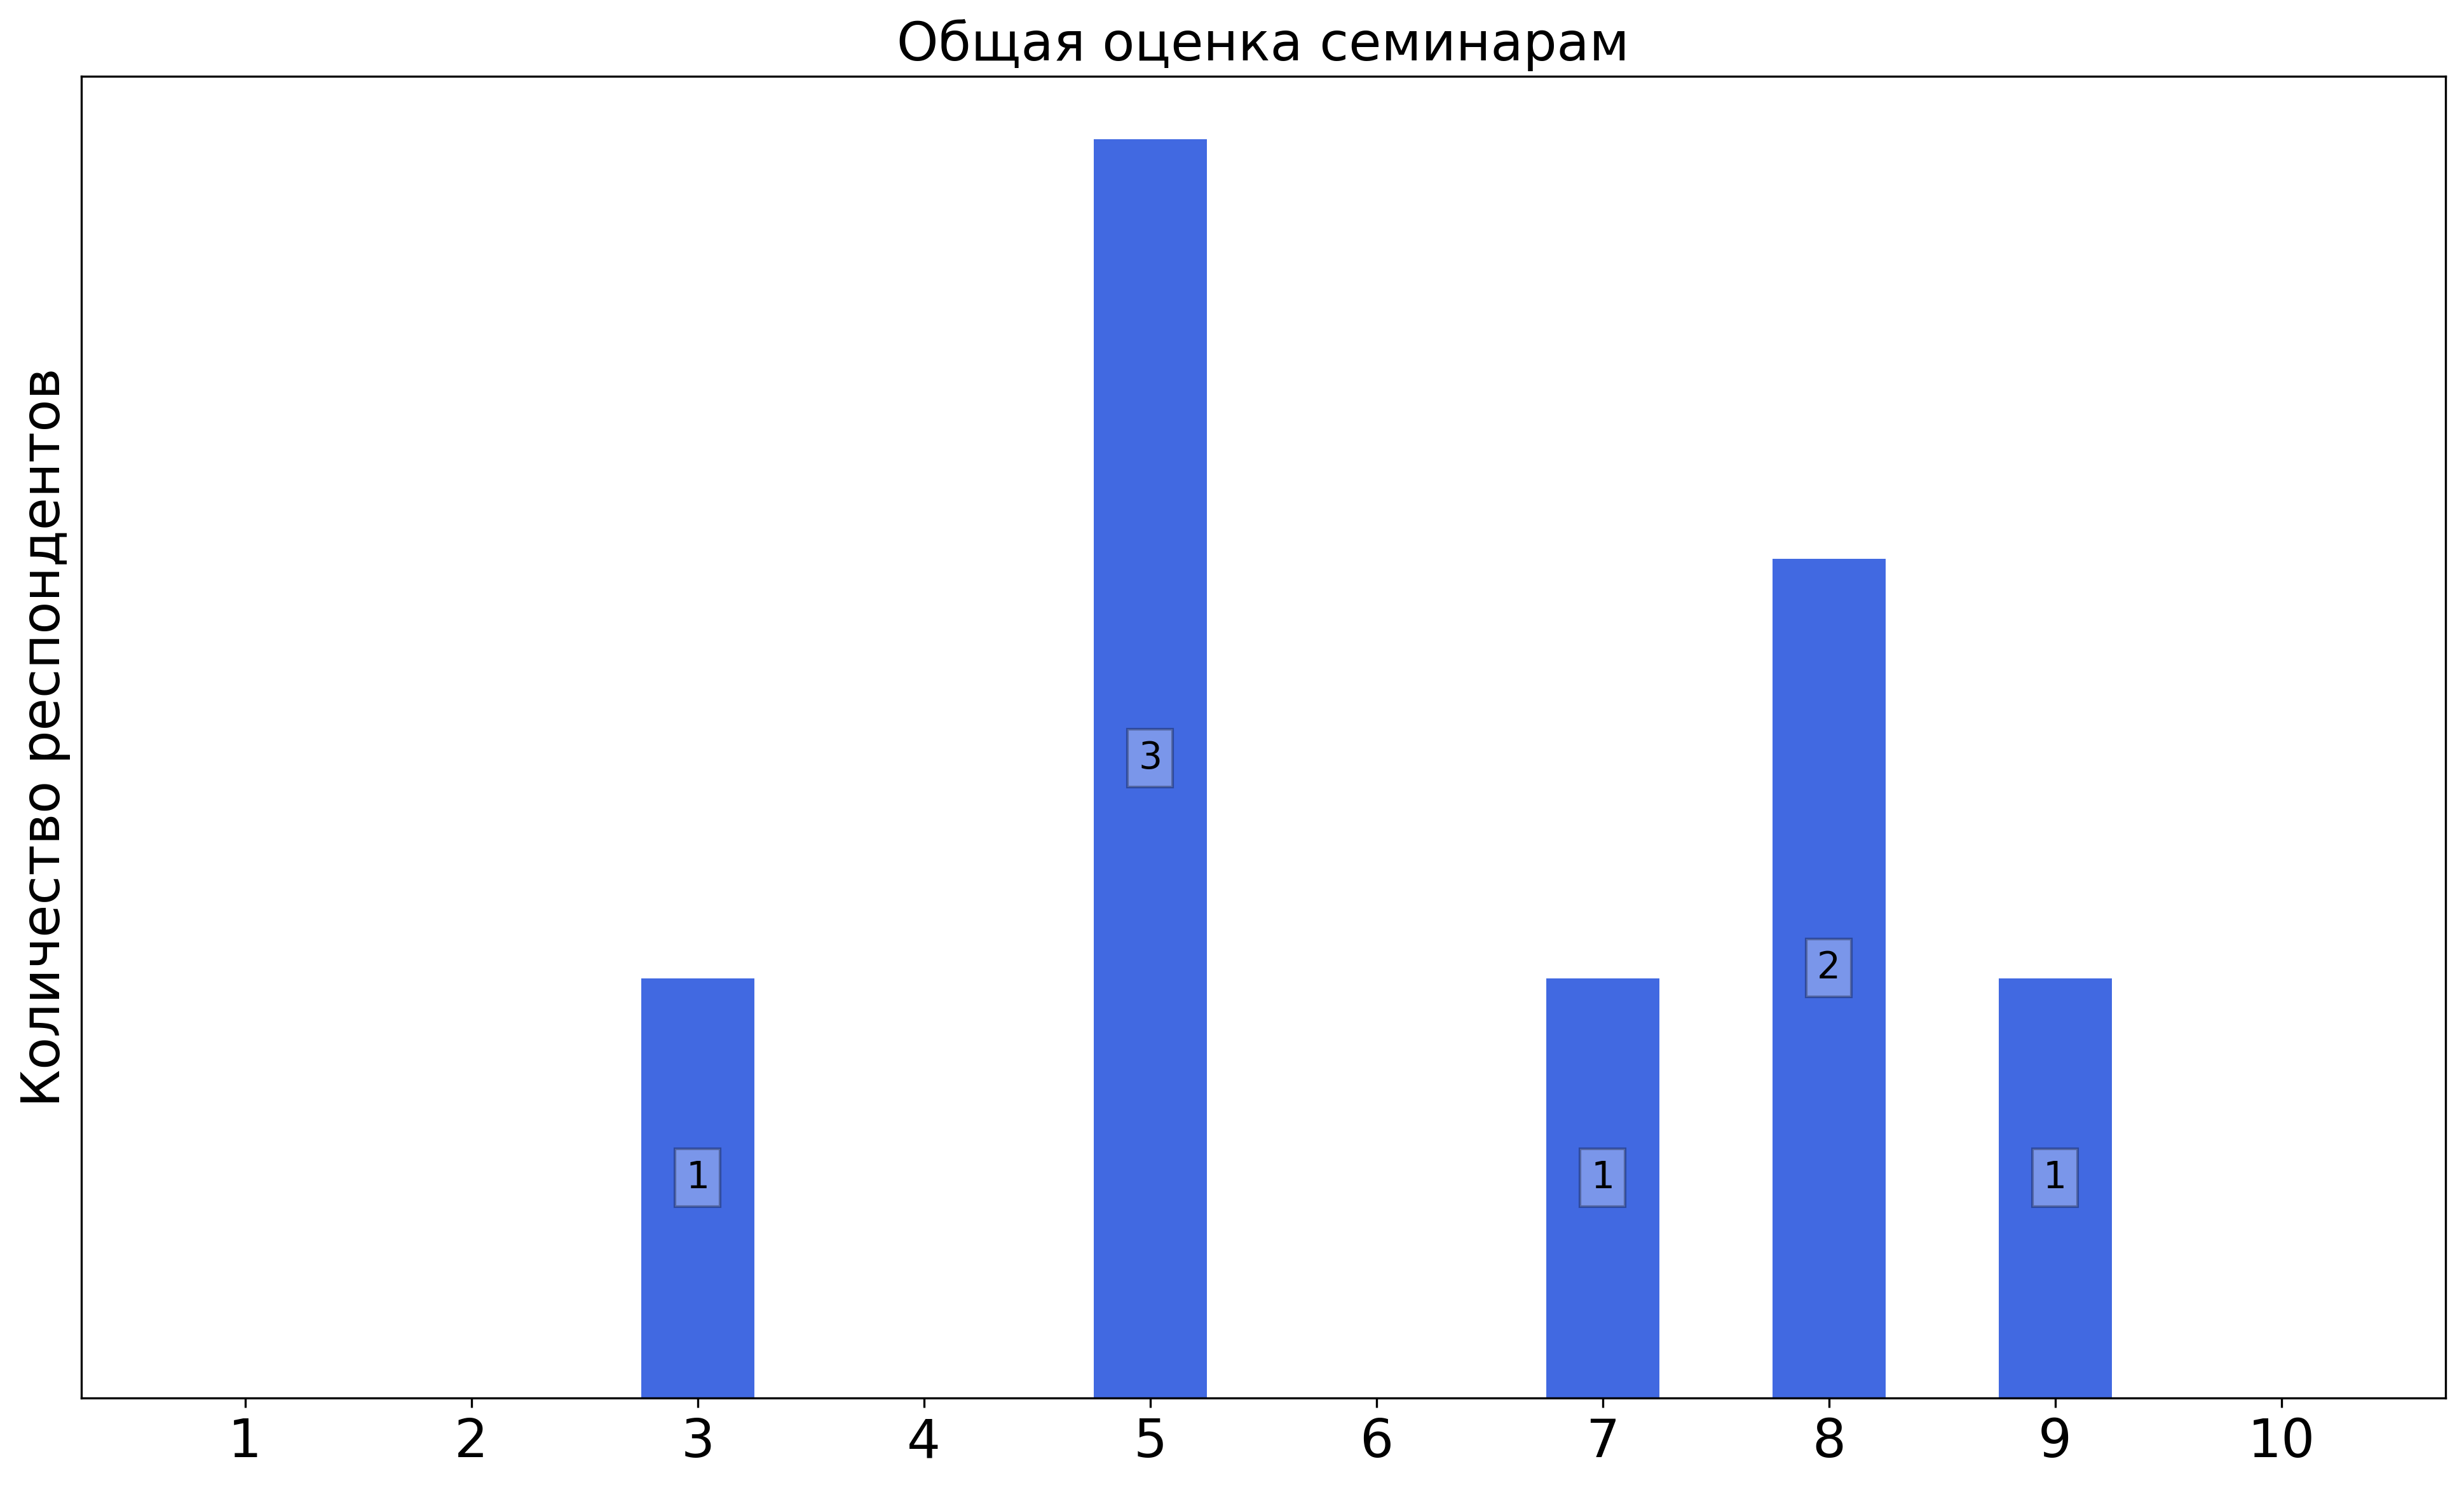
\includegraphics[width=\textwidth]{images/4 course/Введение в машинное обучение/seminarists-marks-Грабовой А.-3.png}
			\end{subfigure}	
			\caption{Оценки респондентов о качестве преподавания семинаров}
		\end{figure}

		\textbf{Комментарии студентов о семинаристе\protect\footnote{сохранены оригинальные орфография и пунктуация}}
            \begin{commentbox} 
                Преподаватель ведет семинары на поток совмещенный из:
                Бакалавриат 3й курс ФПМИ
                Бакалавриат 4й курс ФРКТ
                Магистратура (непонятно какой поток)
                Аспирантура (смешанный)
        
                Он предполагает что у всех есть нужный его семинару мат аппарат и когда РТшники говорят что это не так, он это игнорирует и говорит "так, ну значит все этот предмет изучали, продолжаем" [неиронично, на лекции присутствовало пару десятков ртшников которые подняли руки и в голос сказали что это не так и были проигнорированы]
        
                Кроме 4й курс РТ многие из вышеперечисленных занимаются машинкой профильно, некоторые работают с ней. И да, семинарист опирается именно на них в своем рассказе. И взаимодействует только с ними как с аудиторией 
        
                Шансы понять что-то нет. 
            \end{commentbox}


    \subsubsection{Отзыв студентов о семинарах. Семинарист: Нейчев Р.Г.}
		\begin{figure}[H]
			\centering
			\begin{subfigure}[b]{0.45\textwidth}
				\centering
				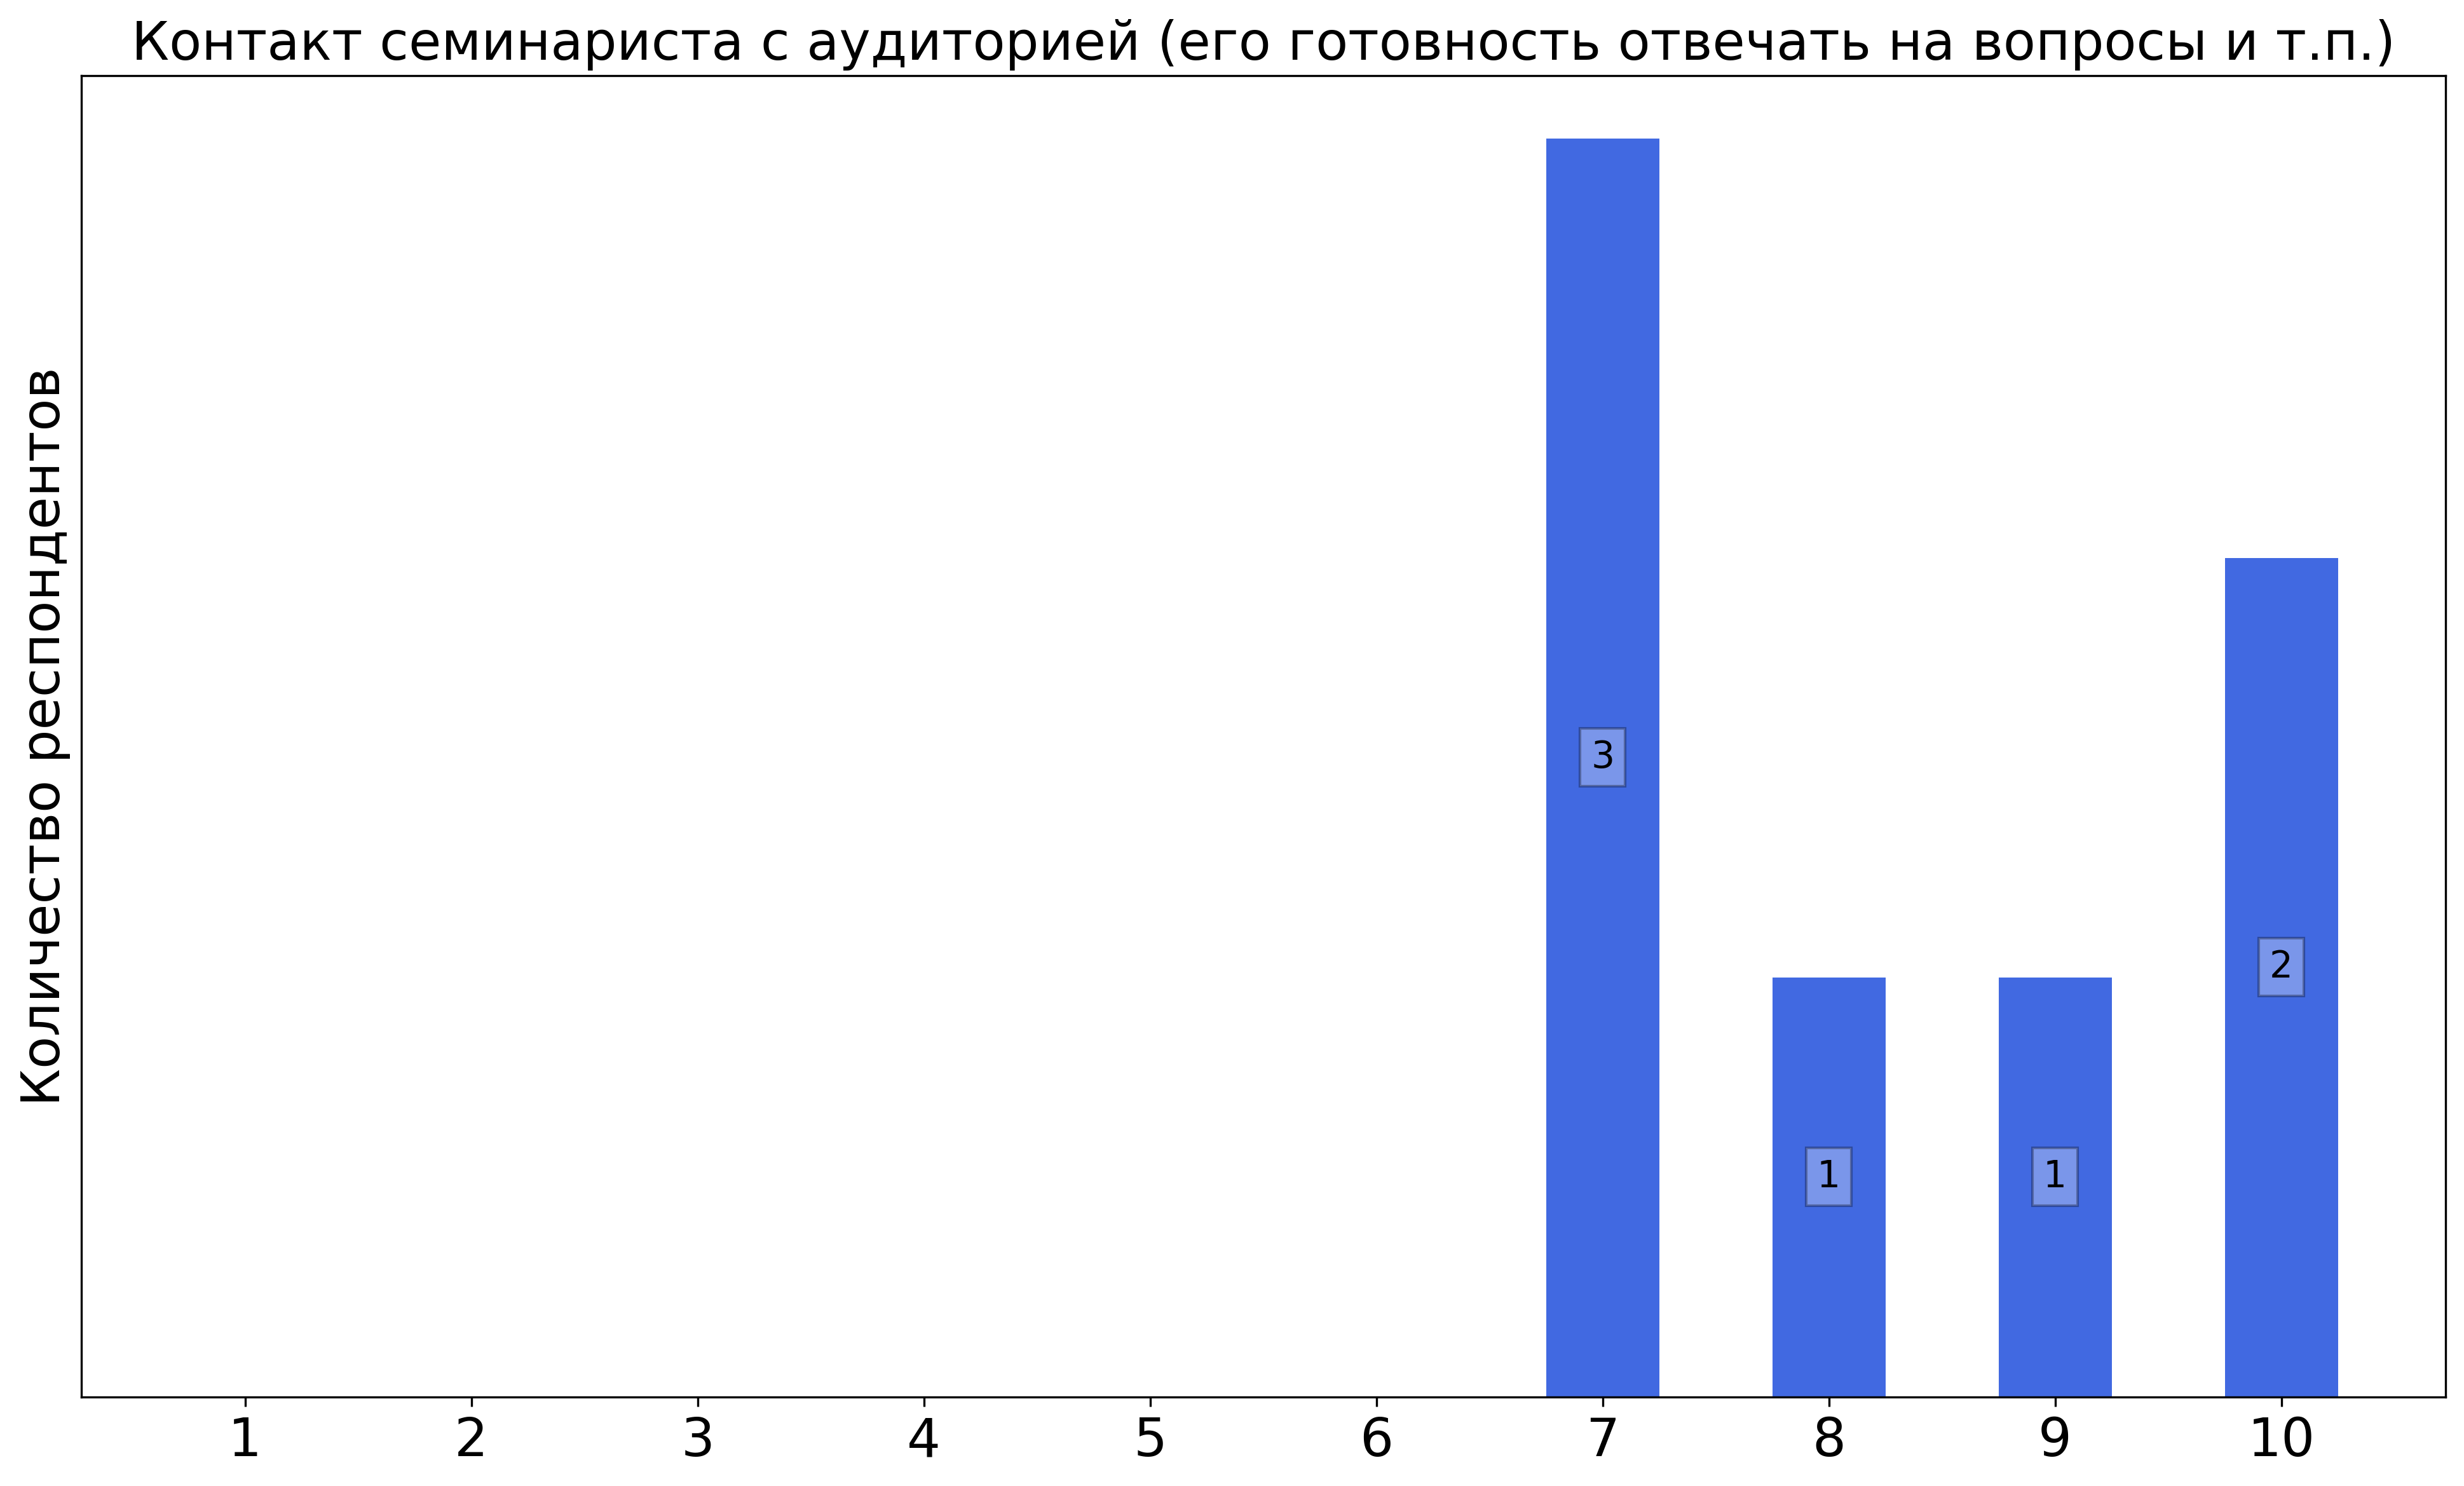
\includegraphics[width=\textwidth]{images/4 course/Введение в машинное обучение/seminarists-marks-Нейчев Р.Г.-0.png}
			\end{subfigure}
			\begin{subfigure}[b]{0.45\textwidth}
				\centering
				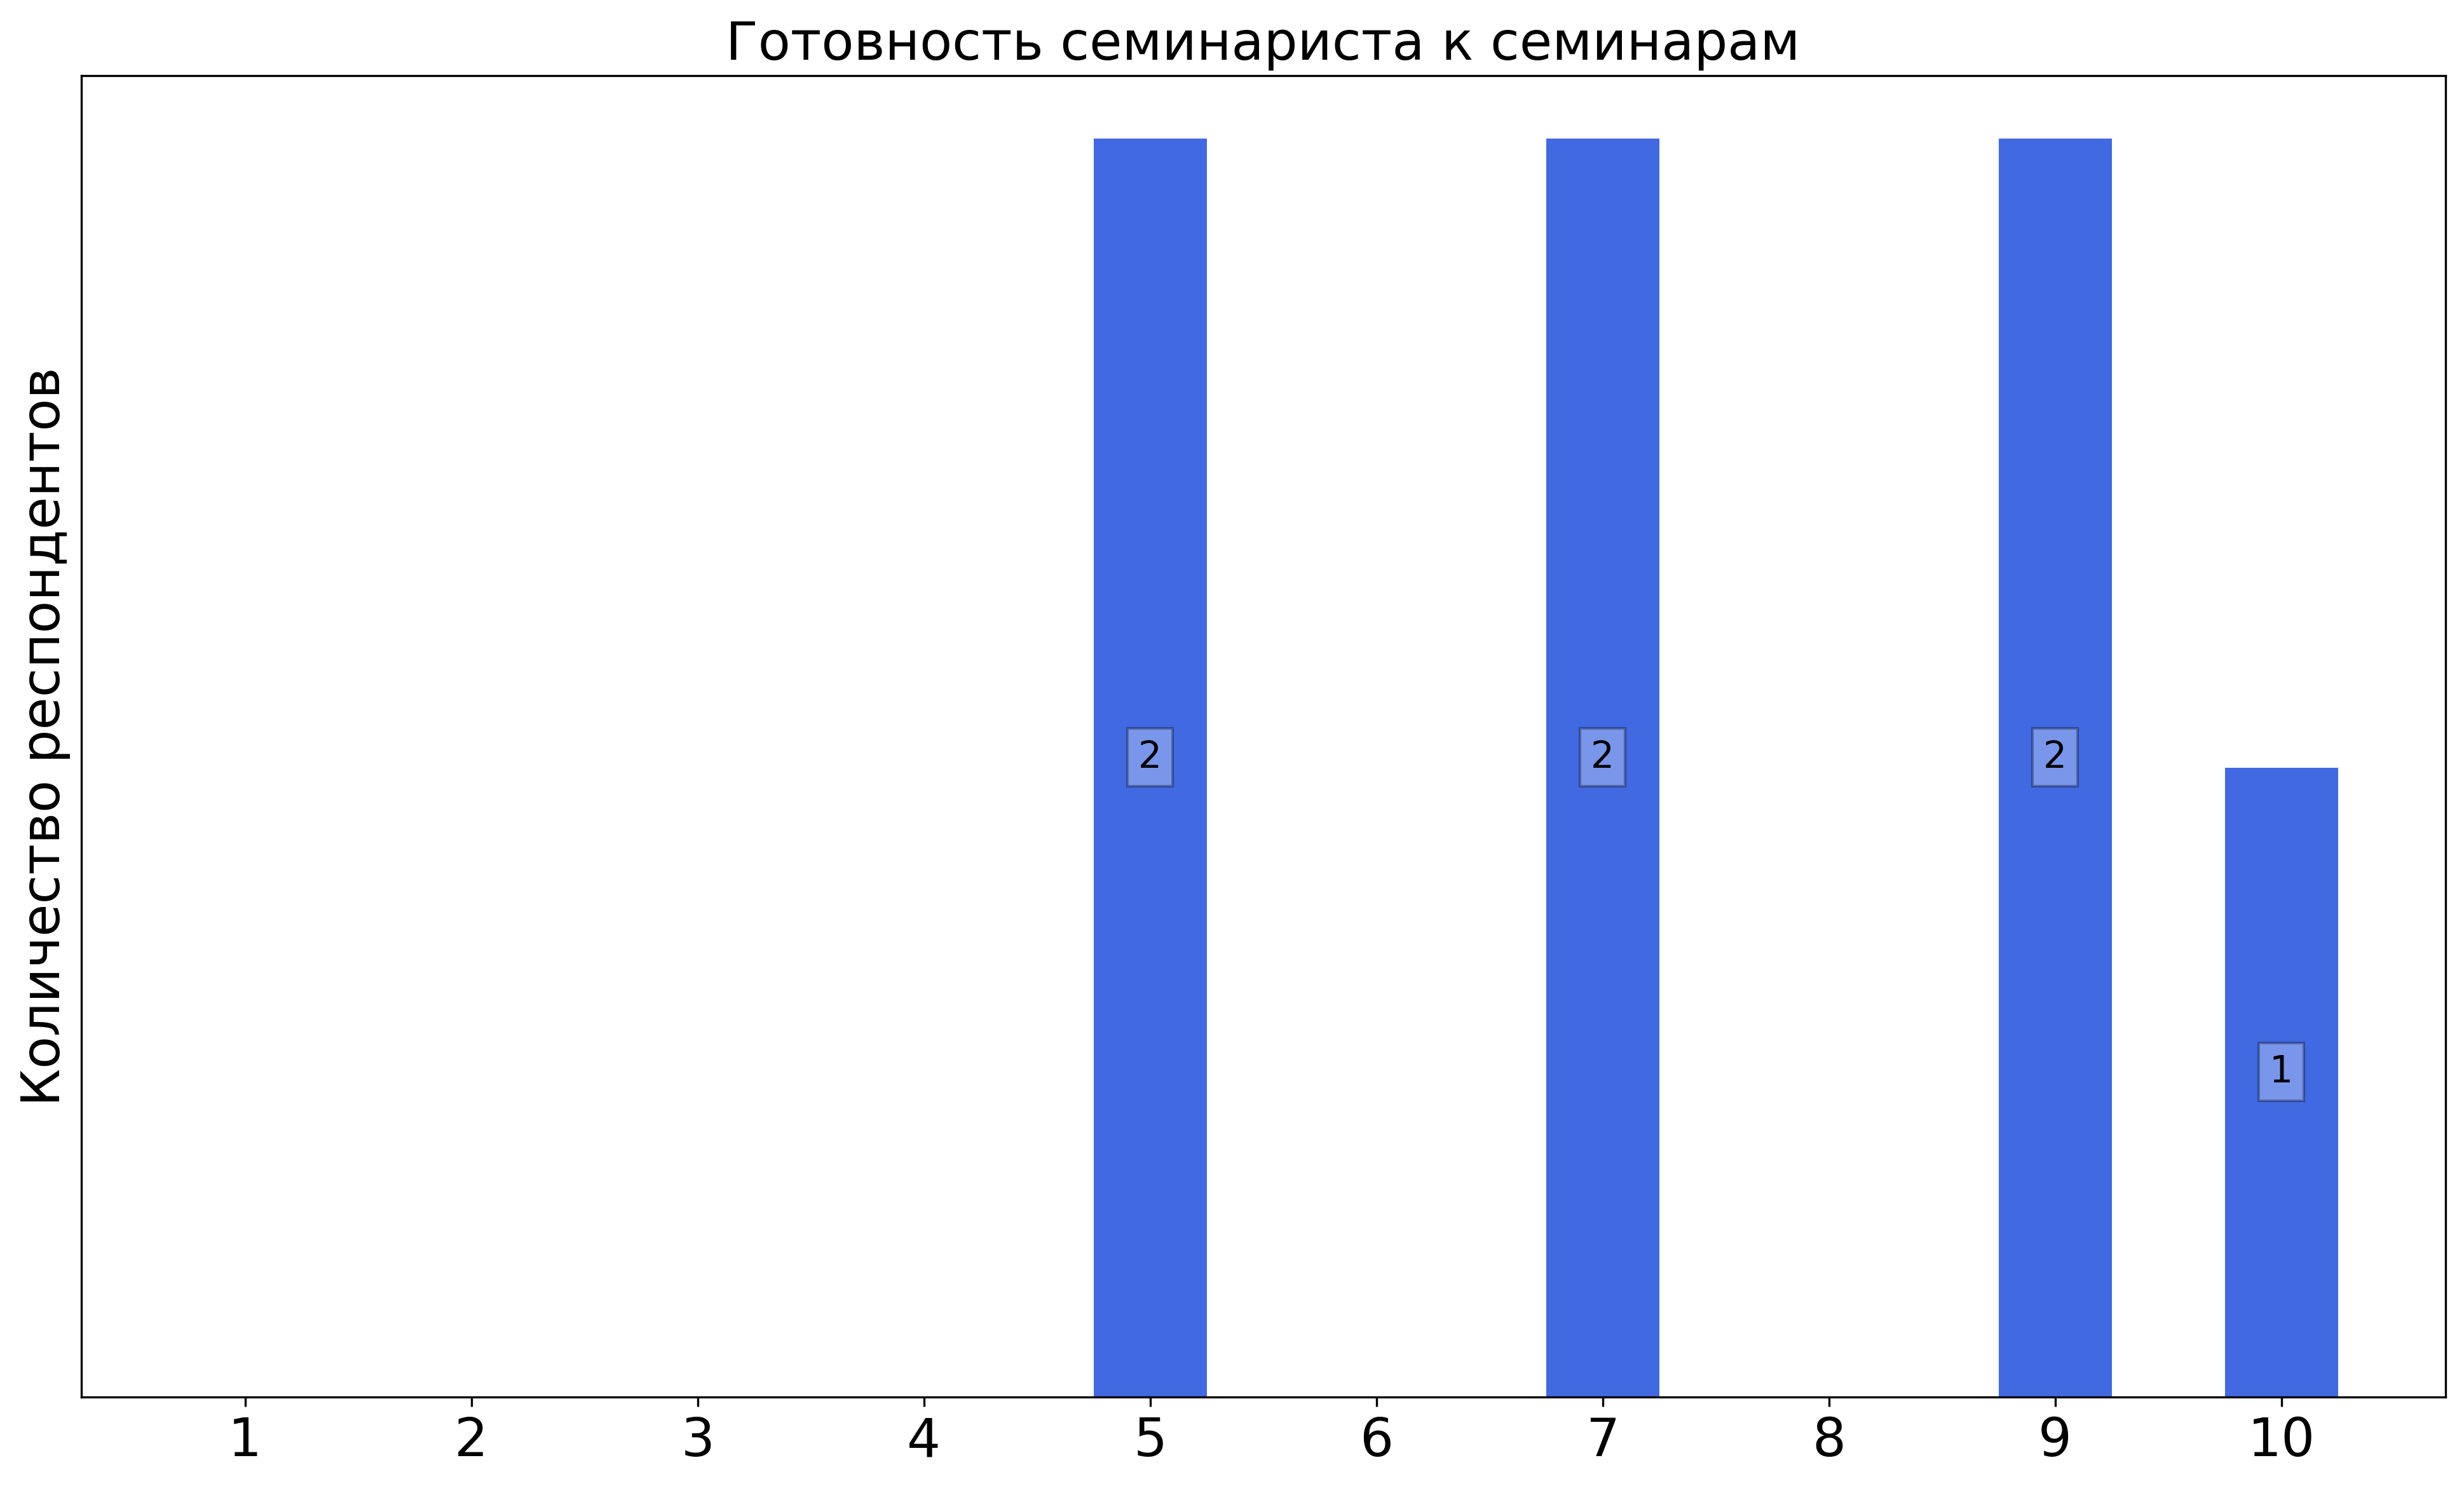
\includegraphics[width=\textwidth]{images/4 course/Введение в машинное обучение/seminarists-marks-Нейчев Р.Г.-1.png}
			\end{subfigure}
			\begin{subfigure}[b]{0.45\textwidth}
				\centering
				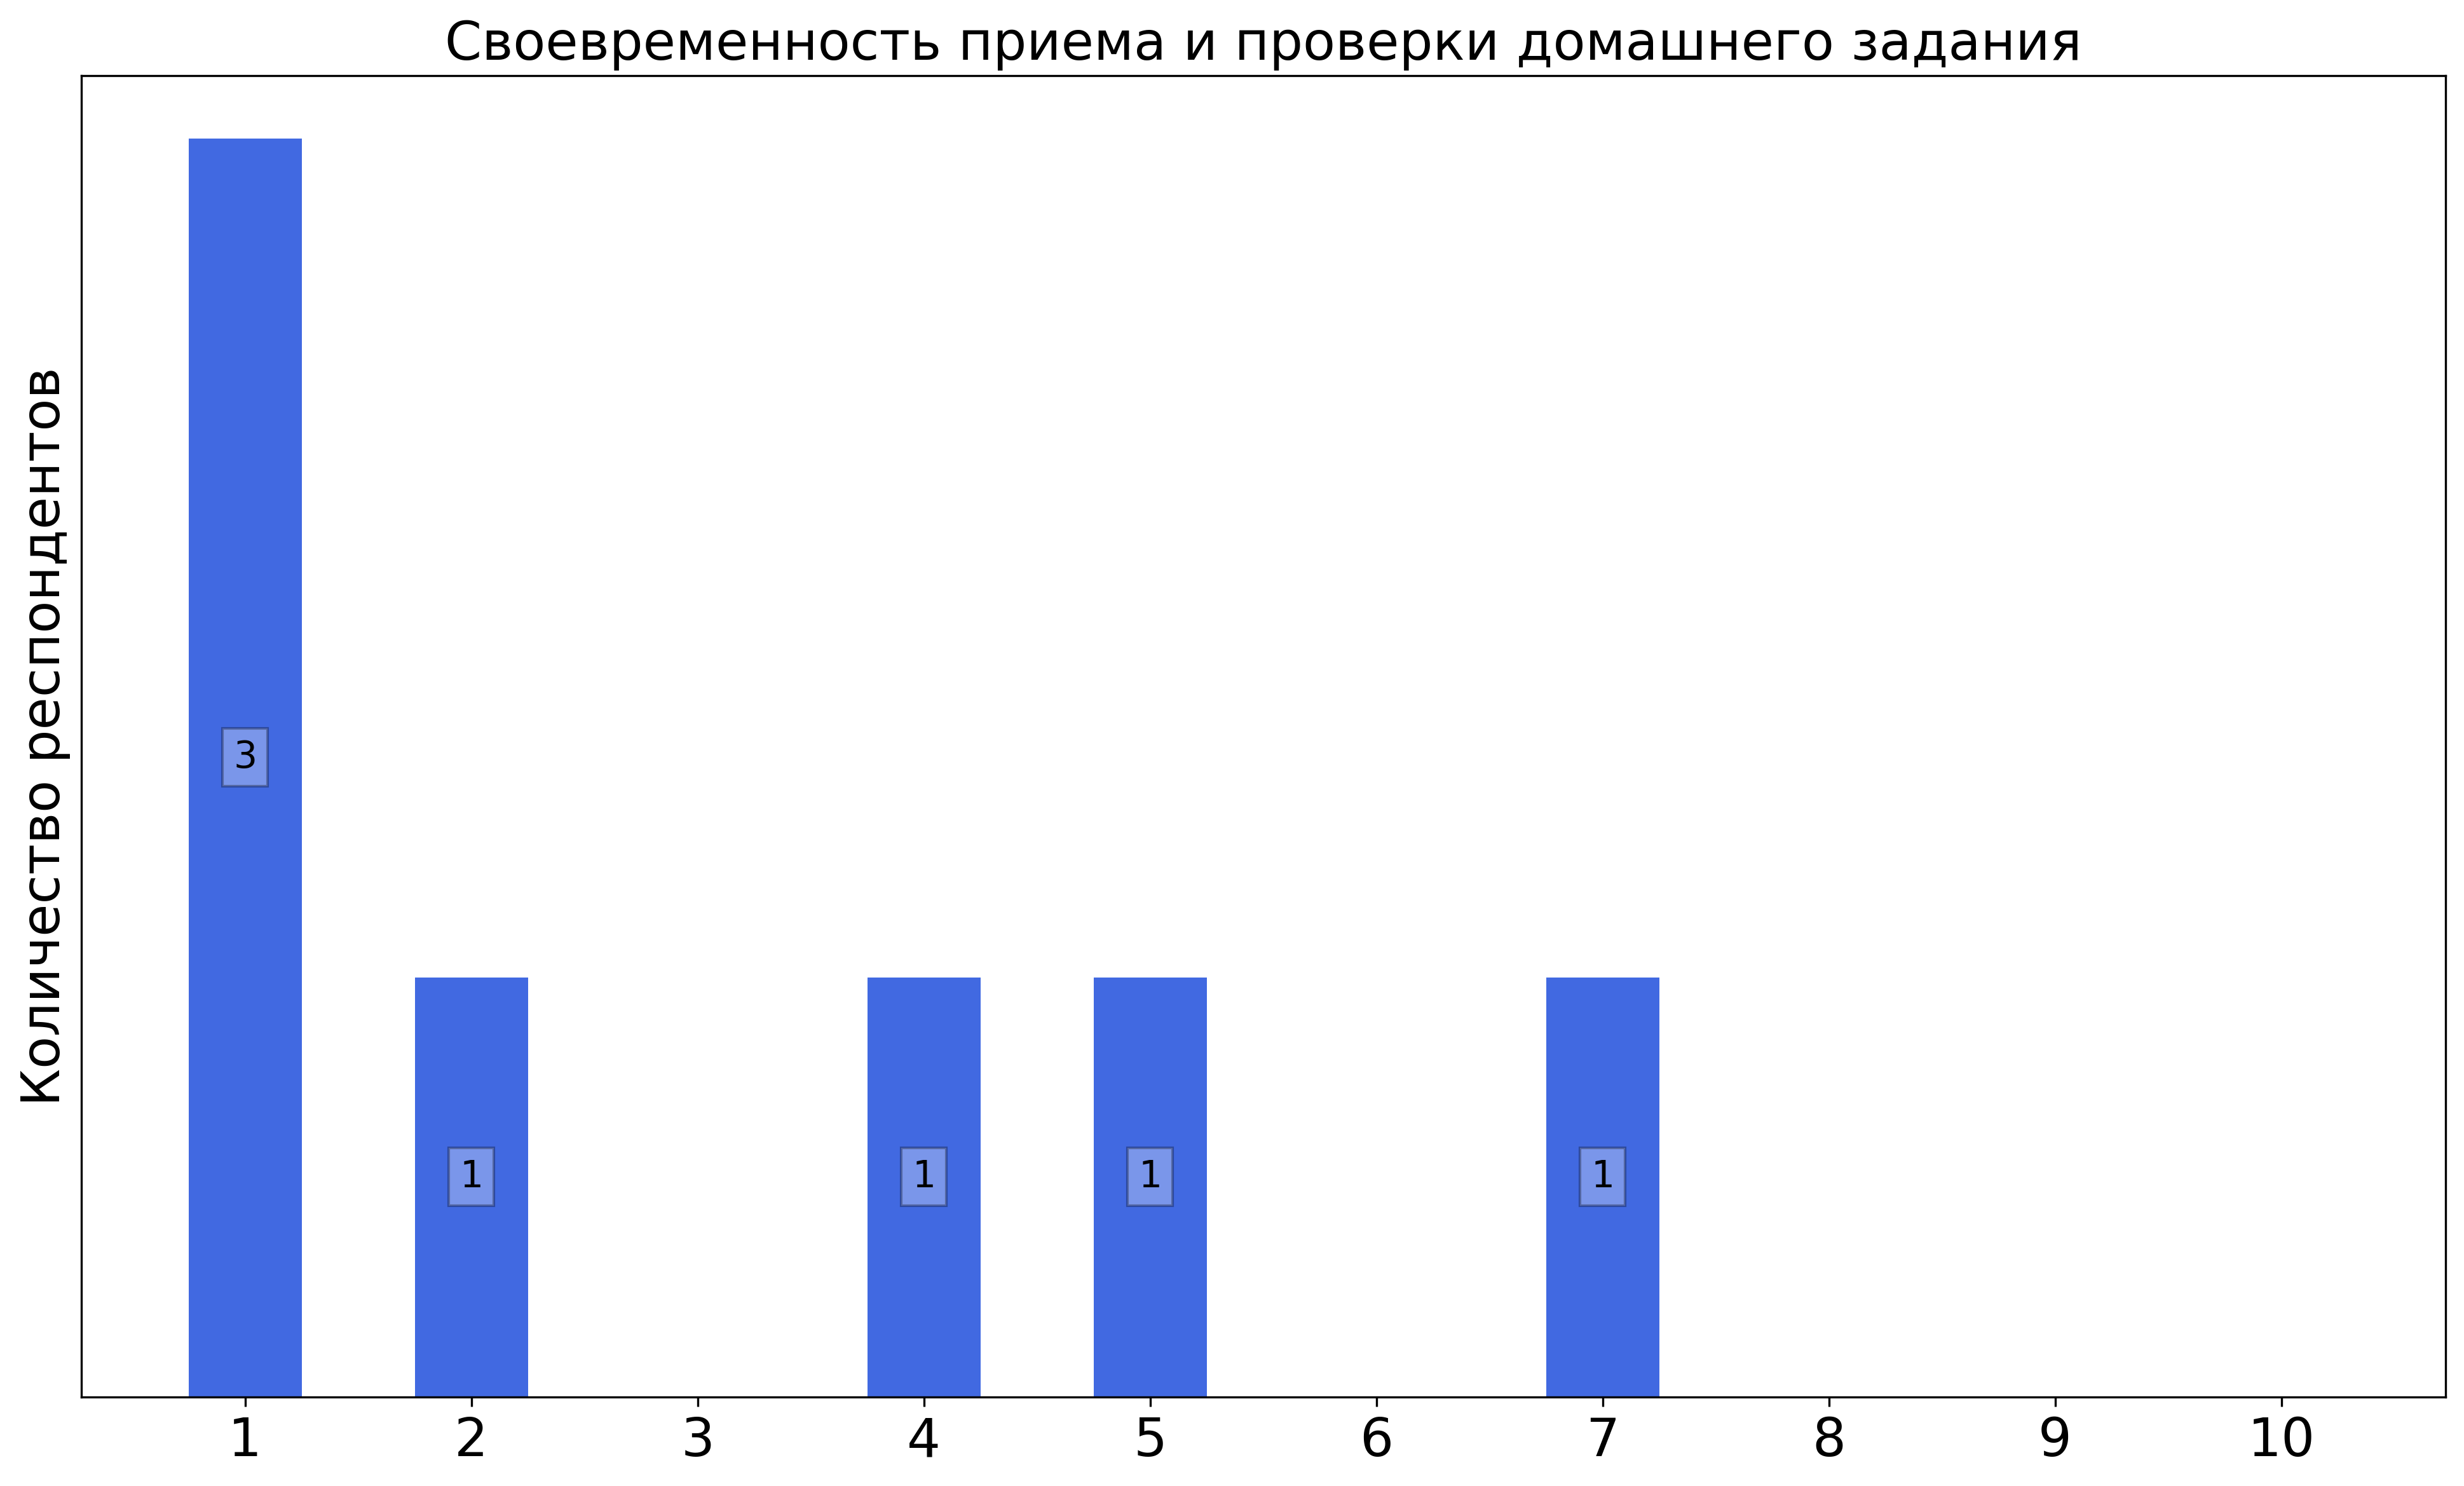
\includegraphics[width=\textwidth]{images/4 course/Введение в машинное обучение/seminarists-marks-Нейчев Р.Г.-2.png}
			\end{subfigure}
			\begin{subfigure}[b]{0.45\textwidth}
				\centering
				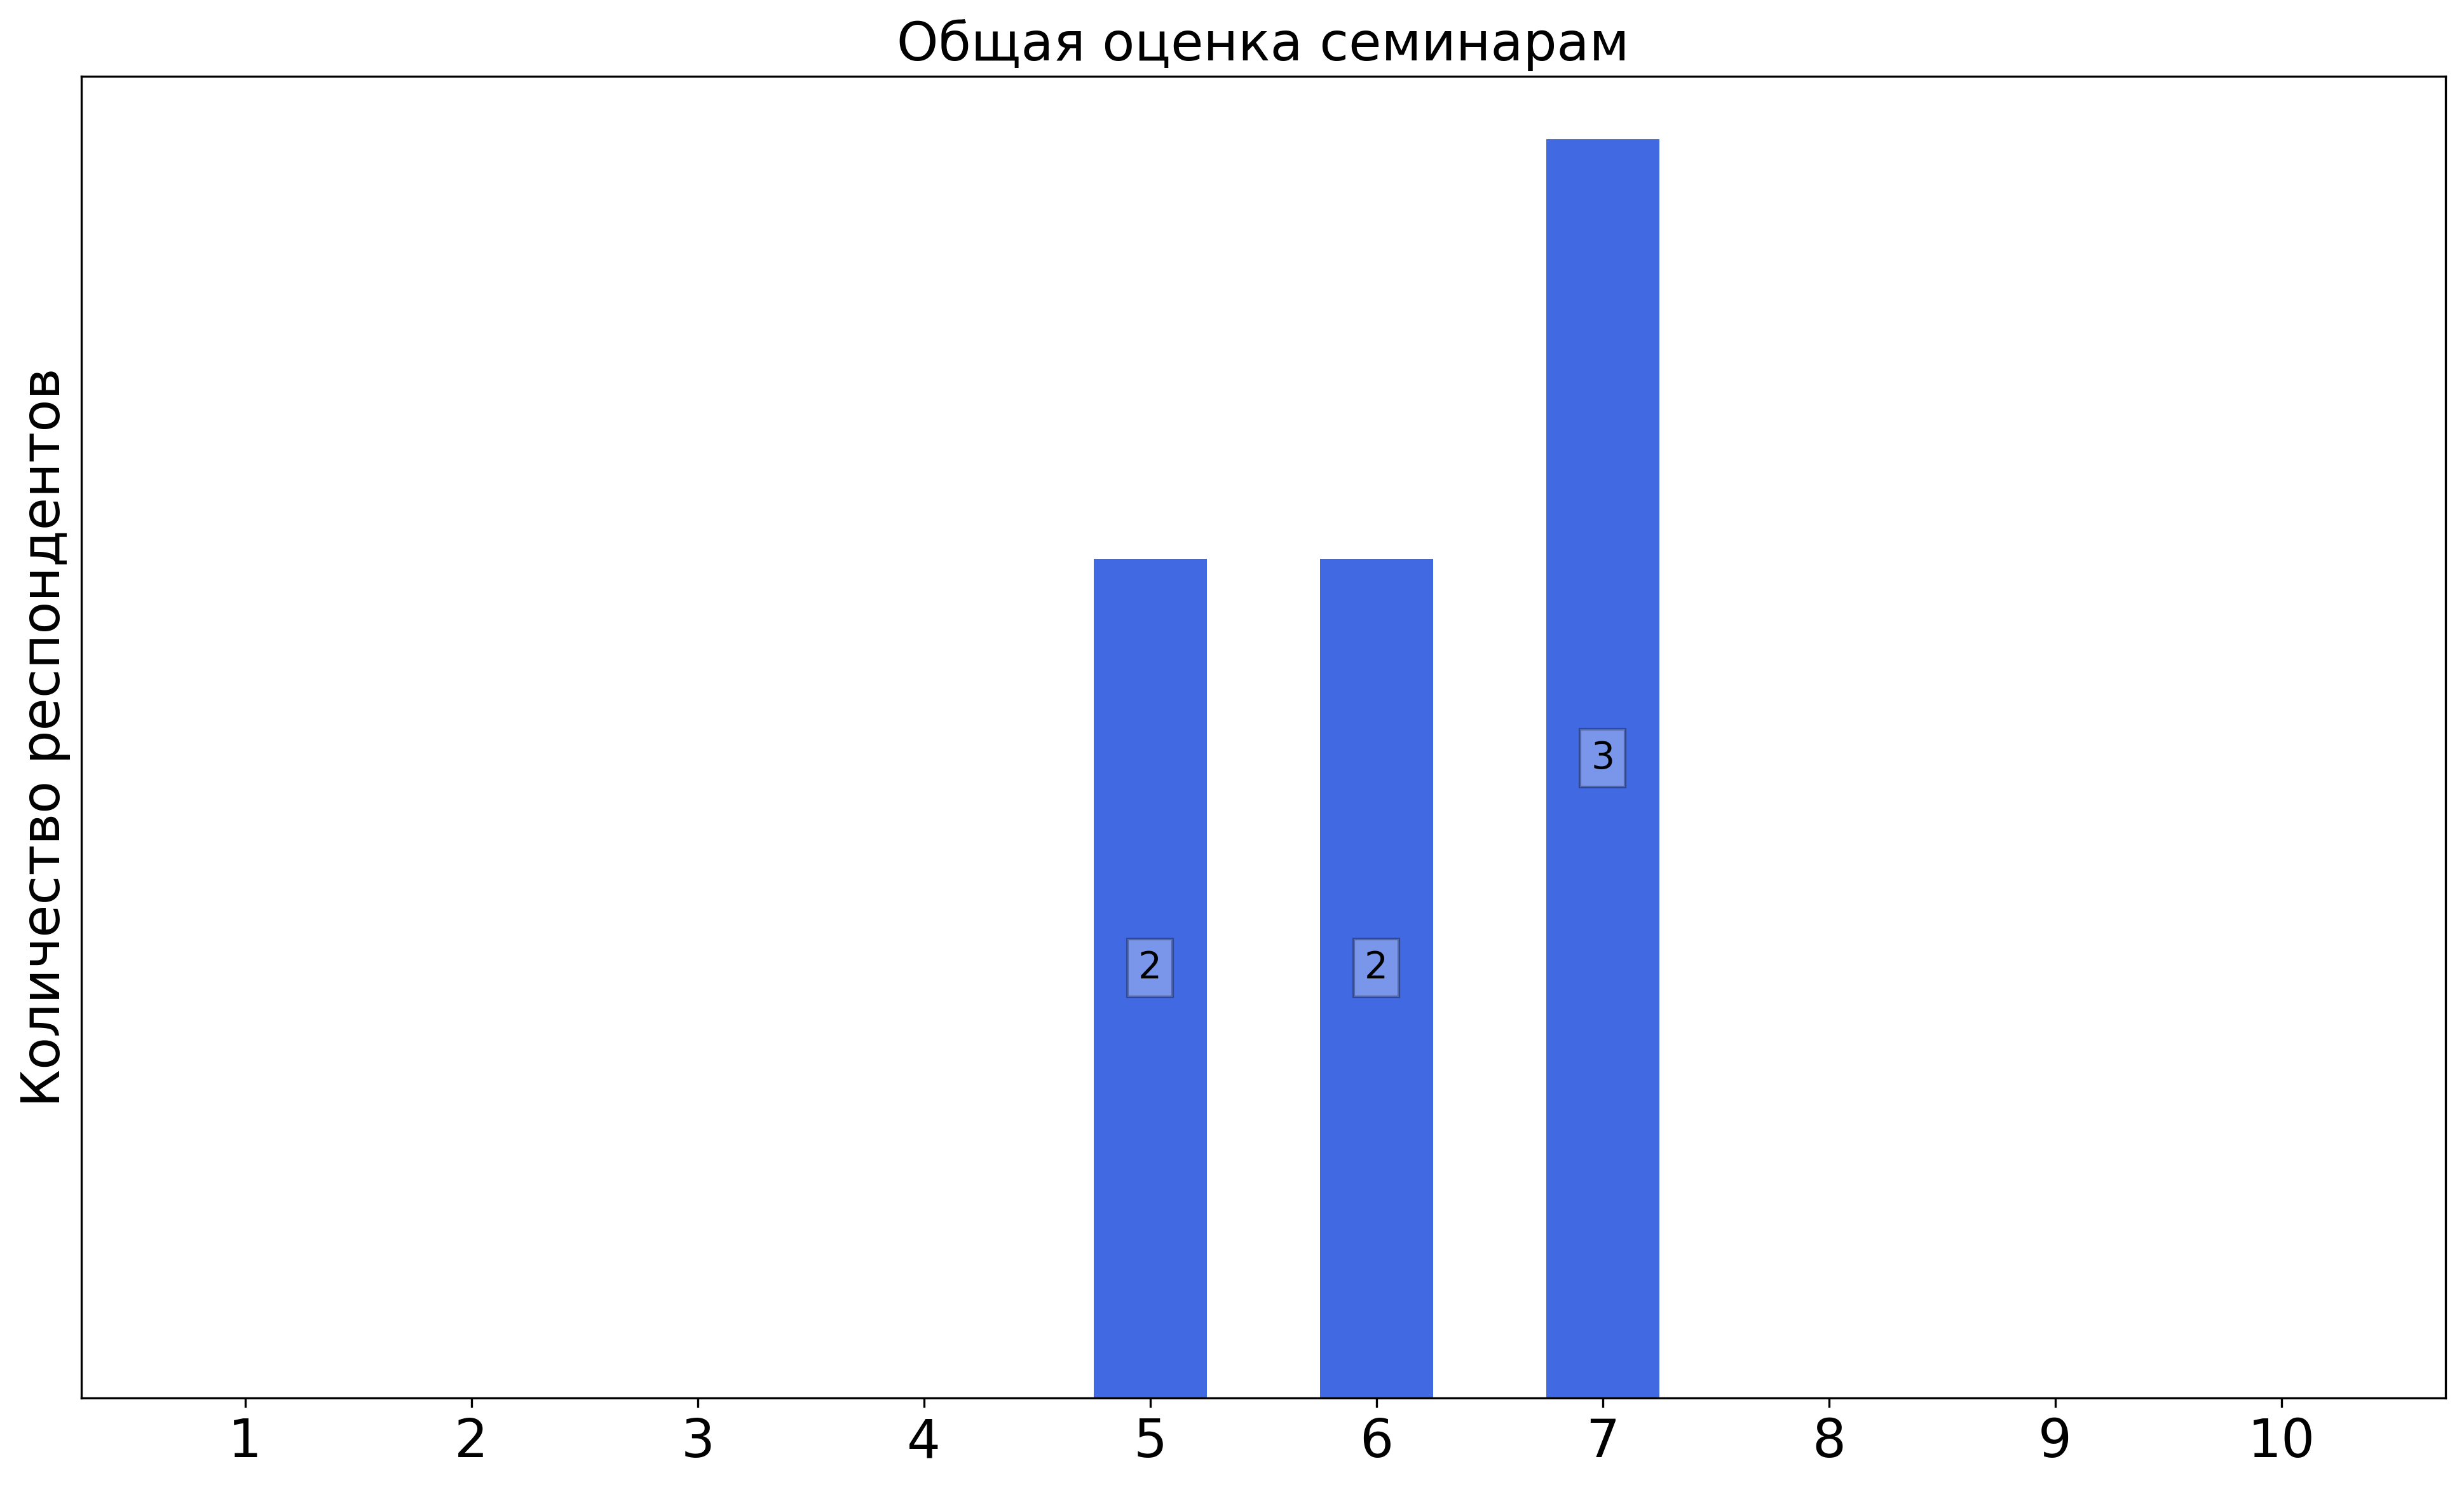
\includegraphics[width=\textwidth]{images/4 course/Введение в машинное обучение/seminarists-marks-Нейчев Р.Г.-3.png}
			\end{subfigure}	
			\caption{Оценки респондентов о качестве преподавания семинаров}
		\end{figure}

		\textbf{Комментарии студентов о семинаристе\protect\footnote{сохранены оригинальные орфография и пунктуация}}
            \begin{commentbox} 
                БольшАя часть семинаров - это были продолжения лекций. На семинарах показываются примеры реализаций. Но для неподготовленного студента это очень тяжело воспринимать, не хватает именно классической семинарской рутины. Большинство домашек было проверено только в январе перед заключительными зачётами, это не очень круто. Дедлайны по домашкам стояли адекватные. Качество оценивания также порадовало. Можно было оспорить свою оценку и повысить 
            \end{commentbox} 
        
            \begin{commentbox} 
                В начале курса было сказано, что домашние задания и тесты на лекциях каким-то образом ограничивают максимальный балл на экзамене. 
        
                В итоге в течение семестра не было ни одного теста на оценку. Домашние работы проверялись крайне несвоевременно. Свои оценки я узнал в три часа ночи в день перед экзаменом. Формулы перевода оценок за домашки в балл не было. Свою "максимальную" оценку я узнал только от экзаменатора.
        
                При этом никаких развернутых комментариев по домашним работам я не получил, поэтому даже не понял в чем были мои ошибки, как их можно не допустить в следующий раз. 
            \end{commentbox} 
        
            \begin{commentbox} 
                На семинары я не ходила, только смотрела некоторые записи семинаров от Нейчева и Гончаренко. И в лекциях и в семинарах мне показалось что Гончаренко больше задерживается на сути вещей, а Нейчев довольно поверхностно рассказывает. 
            \end{commentbox} 
        
            \begin{commentbox} 
                С домашками вышел полнейший ужас. Было заявлено, что домашнее задание будет влиять на оценку на экзамене. При этом к 21.12 - дате проведения зачёта (экзамена) - не была проверена даже первая лаба из трёх. В итоге на зачёте про домашку никто не вспомнил.
                Также были обещаны тесты на лекциях, которые тоже якобы будут влиять на оценку, но их вообще не было.
                А ещё, о том, что экзамен проходит 21.12 мы узнали 18.12. В расписании зачёт должен был состояться 16.12, но его не было.
                Проверка домашнего задания тоже вызывает вопросы. Непонятно, что оценивалось в курсе: интерпретация данных или код. Пока делаешь задание, кажется, что важнее код, а вопросы в конце - для самопроверки. Но оказалось, что вопросы дают наибольший вклад в оценку за лабу.
                Также дата сдачи домашки пару раз передвигалась дальше. В итоге те, кто сдали лабу к первому дедлайну, оказывались в невыгодном положении, тк доделывать её потом времени уже не было. 
            \end{commentbox} 
        
    \subsubsection{Прочие комментарии и предложения по улучшению курса}
        \begin{commentbox}
            Было много неопределенности с домашками, когда они будут, какой вклад вносят, когда будут проверены и тд  
        \end{commentbox}

        \begin{commentbox}
            Очень расплывчатое понимание о проставлении зачётов за курс. Цитата с первой лекции: "никаких автоматов, перезачётов не будет, у всех один экзамен". Итого у половины потока автоматы, половина потока во время экзаменационной сессии сдаёт зачёт, который потом проставляется задним числом
        \end{commentbox}

        \begin{commentbox}
            "Своевременная проверка дз, выкладывание в общий доступ актуальной таблицы оценок.
            Более оперативная публикация записей лекций и семинаров.
            Изменение подхода к семинарам.
            Более понятные критерии финальной оценки за предмет, своевременная публикация программы курса"
        \end{commentbox}

        \begin{commentbox}
            Хотелось бы более прозрачную систему оценивания. По домашним работам хотелось бы иметь возможность задавать вопросы проверяющему.
        \end{commentbox}

        \begin{commentbox}
            Очень бы хотелось увидеть улучшение  организованности курса и по возможности добавление большее полных материалов для подготовки
        \end{commentbox}

        \begin{commentbox}
            Считаю, что подобный курс на рт должен либо быть по выбору, либо отсутствовать вовсе, т.к. машинное обучение необходимо небольшому количеству кафедр, на которых оно уже присутствует в виде базового курса, так же для полного понимания курса необходимо знать и понимать 3 курса: мат. Лог, нормальный теорвер( а недоразумение, что нам преподают) и мат статы. В связи чем  резонно исключить курс, т.к. у 4 курсника рт этих знаний попросту нет
        \end{commentbox}

        \begin{commentbox}
            "Убрать курс как обязательный с РТ. Невозможно изучить этот курс углубленно не на уровне ""так, ну просто запомню, как обезьяна, что чтоб обучить модель надо написать такую функцию"". Почему? Зачем? Как? 

            Ты сможешь понять только если пойдешь поднимать 3 года математики ФУПМ. Чего делать на 4ом курсе уже ни времени ни желания нет.

            Сам семинарист называл 5 предметов которые нужно хорошо знать, чтобы понимать семинары. Ни одного из них на РТ нет. Или, в случае с теорвером, он сильно упрощенный."
        \end{commentbox}

        \begin{commentbox}
            "Очень прошу придумать заранее расписание курса. Я понимаю, что это трудно сделать на 600 человек, но курс идёт уже не первый год.
            Нужно иметь хотя бы какое-то представление о датах. При этом планировать не на 3 дня вперед, а на семестр или хотя бы месяц. Иначе опираться на даты невозможно.
            И огромная просьба соблюдать всё сказанное. А если нет возможности - не говорить этого. Очень много обещаний было не выполнено."
        \end{commentbox}